\documentclass[11pt]{article}

% The four macros of the header standard; tools/zenodo/publish_revision.py patches them when it reserves the DOI.
\newcommand{\doctype}{Preprint}
\newcommand{\docversion}{v1.00.000}
\newcommand{\docdate}{7 November 2026}
\newcommand{\versiondoi}{10.5281/zenodo.0}
\newcommand{\conceptdoi}{10.5281/zenodo.0}
\newcommand{\docidentity}{CAOS\_Contraste, the validation of the risk models of a bank}

% The packages and conventions every Contraste manuscript shares (CAOS_MANAGE conventions/manuscript-content-bar.md
% section 2). A document sets its class, the four header macros and \docidentity, then % The packages and conventions every Contraste manuscript shares (CAOS_MANAGE conventions/manuscript-content-bar.md
% section 2). A document sets its class, the four header macros and \docidentity, then % The packages and conventions every Contraste manuscript shares (CAOS_MANAGE conventions/manuscript-content-bar.md
% section 2). A document sets its class, the four header macros and \docidentity, then \input{../_shared/preamble}.
\usepackage[T1]{fontenc}
\usepackage[utf8]{inputenc}
\usepackage{lmodern}
\usepackage{microtype}
\usepackage[a4paper,margin=2.5cm]{geometry}
\usepackage{amsmath,amssymb,amsthm,mathtools,bm}
\usepackage{graphicx}
\usepackage{booktabs,longtable,tabularx,array,multirow}
\usepackage{siunitx}
\usepackage{algorithm}
\usepackage{algpseudocode}
\usepackage{caption,subcaption}
\usepackage{xcolor}
\usepackage[numbers,sort&compress]{natbib}
\usepackage[hidelinks]{hyperref}
\usepackage{cleveref}
\usepackage{orcidlink}

\sisetup{group-separator={,},group-minimum-digits=4,detect-all}
\graphicspath{{figures/}{../figures/}}
\captionsetup{font=small,labelfont=bf}
\setlength{\LTcapwidth}{\textwidth}

% Theorem environments for the Theory sections of the manuscripts.
\newtheorem{proposition}{Proposition}
\newtheorem{lemma}{Lemma}
\newtheorem{corollary}{Corollary}
\theoremstyle{definition}
\newtheorem{definition}{Definition}
\newtheorem{assumption}{Assumption}
\theoremstyle{remark}
\newtheorem{remark}{Remark}

% Notation shared by the documents (each defines it again in its notation table).
\newcommand{\E}{\mathbb{E}}
\newcommand{\Prob}{\mathbb{P}}
\newcommand{\Var}{\operatorname{Var}}
\newcommand{\Cov}{\operatorname{Cov}}
\newcommand{\VaR}{\operatorname{VaR}}
\newcommand{\ES}{\operatorname{ES}}
\newcommand{\PD}{\mathrm{PD}}
\newcommand{\LGD}{\mathrm{LGD}}
\newcommand{\EAD}{\mathrm{EAD}}
\newcommand{\ECL}{\mathrm{ECL}}
\newcommand{\indic}{\mathbf{1}}
\newcommand{\R}{\mathbb{R}}
\newcommand{\dd}{\,\mathrm{d}}

% The page-1 header block (CAOS_MANAGE conventions/manuscript-header-standard.md). The document defines \doctype,
% \docversion, \docdate, \versiondoi, \conceptdoi and \docidentity before this file; the publishing tool patches the four
% macros of the standard when it reserves the version DOI.
\newcommand{\docrepo}{github.com/fsantibanezleal/CAOS\_Contraste}
\newcommand{\headerblock}{%
\begin{center}
\fbox{\parbox{0.94\textwidth}{\small\raggedright
\textbf{\doctype} \quad$\cdot$\quad \docversion, \docdate \quad$\cdot$\quad Licence CC BY 4.0\\[2pt]
CAOS open-research programme \quad$\cdot$\quad \docidentity\\[2pt]
Version DOI \href{https://doi.org/\versiondoi}{\texttt{\versiondoi}} \quad$\cdot$\quad
concept DOI (always latest) \href{https://doi.org/\conceptdoi}{\texttt{\conceptdoi}}\\[2pt]
Not peer reviewed. Source code, data and computational records: \href{https://\docrepo}{\texttt{\docrepo}}
}}
\end{center}
\vspace{4pt}}
.
\usepackage[T1]{fontenc}
\usepackage[utf8]{inputenc}
\usepackage{lmodern}
\usepackage{microtype}
\usepackage[a4paper,margin=2.5cm]{geometry}
\usepackage{amsmath,amssymb,amsthm,mathtools,bm}
\usepackage{graphicx}
\usepackage{booktabs,longtable,tabularx,array,multirow}
\usepackage{siunitx}
\usepackage{algorithm}
\usepackage{algpseudocode}
\usepackage{caption,subcaption}
\usepackage{xcolor}
\usepackage[numbers,sort&compress]{natbib}
\usepackage[hidelinks]{hyperref}
\usepackage{cleveref}
\usepackage{orcidlink}

\sisetup{group-separator={,},group-minimum-digits=4,detect-all}
\graphicspath{{figures/}{../figures/}}
\captionsetup{font=small,labelfont=bf}
\setlength{\LTcapwidth}{\textwidth}

% Theorem environments for the Theory sections of the manuscripts.
\newtheorem{proposition}{Proposition}
\newtheorem{lemma}{Lemma}
\newtheorem{corollary}{Corollary}
\theoremstyle{definition}
\newtheorem{definition}{Definition}
\newtheorem{assumption}{Assumption}
\theoremstyle{remark}
\newtheorem{remark}{Remark}

% Notation shared by the documents (each defines it again in its notation table).
\newcommand{\E}{\mathbb{E}}
\newcommand{\Prob}{\mathbb{P}}
\newcommand{\Var}{\operatorname{Var}}
\newcommand{\Cov}{\operatorname{Cov}}
\newcommand{\VaR}{\operatorname{VaR}}
\newcommand{\ES}{\operatorname{ES}}
\newcommand{\PD}{\mathrm{PD}}
\newcommand{\LGD}{\mathrm{LGD}}
\newcommand{\EAD}{\mathrm{EAD}}
\newcommand{\ECL}{\mathrm{ECL}}
\newcommand{\indic}{\mathbf{1}}
\newcommand{\R}{\mathbb{R}}
\newcommand{\dd}{\,\mathrm{d}}

% The page-1 header block (CAOS_MANAGE conventions/manuscript-header-standard.md). The document defines \doctype,
% \docversion, \docdate, \versiondoi, \conceptdoi and \docidentity before this file; the publishing tool patches the four
% macros of the standard when it reserves the version DOI.
\newcommand{\docrepo}{github.com/fsantibanezleal/CAOS\_Contraste}
\newcommand{\headerblock}{%
\begin{center}
\fbox{\parbox{0.94\textwidth}{\small\raggedright
\textbf{\doctype} \quad$\cdot$\quad \docversion, \docdate \quad$\cdot$\quad Licence CC BY 4.0\\[2pt]
CAOS open-research programme \quad$\cdot$\quad \docidentity\\[2pt]
Version DOI \href{https://doi.org/\versiondoi}{\texttt{\versiondoi}} \quad$\cdot$\quad
concept DOI (always latest) \href{https://doi.org/\conceptdoi}{\texttt{\conceptdoi}}\\[2pt]
Not peer reviewed. Source code, data and computational records: \href{https://\docrepo}{\texttt{\docrepo}}
}}
\end{center}
\vspace{4pt}}
.
\usepackage[T1]{fontenc}
\usepackage[utf8]{inputenc}
\usepackage{lmodern}
\usepackage{microtype}
\usepackage[a4paper,margin=2.5cm]{geometry}
\usepackage{amsmath,amssymb,amsthm,mathtools,bm}
\usepackage{graphicx}
\usepackage{booktabs,longtable,tabularx,array,multirow}
\usepackage{siunitx}
\usepackage{algorithm}
\usepackage{algpseudocode}
\usepackage{caption,subcaption}
\usepackage{xcolor}
\usepackage[numbers,sort&compress]{natbib}
\usepackage[hidelinks]{hyperref}
\usepackage{cleveref}
\usepackage{orcidlink}

\sisetup{group-separator={,},group-minimum-digits=4,detect-all}
\graphicspath{{figures/}{../figures/}}
\captionsetup{font=small,labelfont=bf}
\setlength{\LTcapwidth}{\textwidth}

% Theorem environments for the Theory sections of the manuscripts.
\newtheorem{proposition}{Proposition}
\newtheorem{lemma}{Lemma}
\newtheorem{corollary}{Corollary}
\theoremstyle{definition}
\newtheorem{definition}{Definition}
\newtheorem{assumption}{Assumption}
\theoremstyle{remark}
\newtheorem{remark}{Remark}

% Notation shared by the documents (each defines it again in its notation table).
\newcommand{\E}{\mathbb{E}}
\newcommand{\Prob}{\mathbb{P}}
\newcommand{\Var}{\operatorname{Var}}
\newcommand{\Cov}{\operatorname{Cov}}
\newcommand{\VaR}{\operatorname{VaR}}
\newcommand{\ES}{\operatorname{ES}}
\newcommand{\PD}{\mathrm{PD}}
\newcommand{\LGD}{\mathrm{LGD}}
\newcommand{\EAD}{\mathrm{EAD}}
\newcommand{\ECL}{\mathrm{ECL}}
\newcommand{\indic}{\mathbf{1}}
\newcommand{\R}{\mathbb{R}}
\newcommand{\dd}{\,\mathrm{d}}

% The page-1 header block (CAOS_MANAGE conventions/manuscript-header-standard.md). The document defines \doctype,
% \docversion, \docdate, \versiondoi, \conceptdoi and \docidentity before this file; the publishing tool patches the four
% macros of the standard when it reserves the version DOI.
\newcommand{\docrepo}{github.com/fsantibanezleal/CAOS\_Contraste}
\newcommand{\headerblock}{%
\begin{center}
\fbox{\parbox{0.94\textwidth}{\small\raggedright
\textbf{\doctype} \quad$\cdot$\quad \docversion, \docdate \quad$\cdot$\quad Licence CC BY 4.0\\[2pt]
CAOS open-research programme \quad$\cdot$\quad \docidentity\\[2pt]
Version DOI \href{https://doi.org/\versiondoi}{\texttt{\versiondoi}} \quad$\cdot$\quad
concept DOI (always latest) \href{https://doi.org/\conceptdoi}{\texttt{\conceptdoi}}\\[2pt]
Not peer reviewed. Source code, data and computational records: \href{https://\docrepo}{\texttt{\docrepo}}
}}
\end{center}
\vspace{4pt}}


% Statements of the Theory section that the shared preamble does not define.
\theoremstyle{plain}
\newtheorem{conjecture}{Conjecture}

% Every number quoted from an experiment is read from tables/numbers.tex, which make_artifacts.py writes from the committed outputs.
\makeatletter
% generated by make_artifacts.py: do not edit
\expandafter\def\csname num@abl.G1.fa\endcsname{0}
\expandafter\def\csname num@abl.G1.full\endcsname{9}
\expandafter\def\csname num@abl.G1.mean\endcsname{69.5}
\expandafter\def\csname num@abl.G1.never\endcsname{4}
\expandafter\def\csname num@abl.G1G2.fa\endcsname{0}
\expandafter\def\csname num@abl.G1G2.full\endcsname{14}
\expandafter\def\csname num@abl.G1G2.mean\endcsname{99.9}
\expandafter\def\csname num@abl.G1G2.never\endcsname{0}
\expandafter\def\csname num@abl.G1G2G3.fa\endcsname{0}
\expandafter\def\csname num@abl.G1G2G3.full\endcsname{15}
\expandafter\def\csname num@abl.G1G2G3.mean\endcsname{100.0}
\expandafter\def\csname num@abl.G1G2G3.never\endcsname{0}
\expandafter\def\csname num@abl.G1G3.fa\endcsname{0}
\expandafter\def\csname num@abl.G1G3.full\endcsname{14}
\expandafter\def\csname num@abl.G1G3.mean\endcsname{98.0}
\expandafter\def\csname num@abl.G1G3.never\endcsname{0}
\expandafter\def\csname num@abl.G2.fa\endcsname{0}
\expandafter\def\csname num@abl.G2.full\endcsname{10}
\expandafter\def\csname num@abl.G2.mean\endcsname{73.3}
\expandafter\def\csname num@abl.G2.never\endcsname{4}
\expandafter\def\csname num@abl.G2G3.fa\endcsname{0}
\expandafter\def\csname num@abl.G2G3.full\endcsname{15}
\expandafter\def\csname num@abl.G2G3.mean\endcsname{100.0}
\expandafter\def\csname num@abl.G2G3.never\endcsname{0}
\expandafter\def\csname num@abl.G3.fa\endcsname{0}
\expandafter\def\csname num@abl.G3.full\endcsname{13}
\expandafter\def\csname num@abl.G3.mean\endcsname{95.9}
\expandafter\def\csname num@abl.G3.never\endcsname{0}
\expandafter\def\csname num@c01.cal\endcsname{4,200}
\expandafter\def\csname num@c01.hold\endcsname{9,000}
\expandafter\def\csname num@c01.holdev\endcsname{1,991}
\expandafter\def\csname num@c01.rate\endcsname{22.1}
\expandafter\def\csname num@c01.train\endcsname{16,800}
\expandafter\def\csname num@c02.h1.ev\endcsname{123}
\expandafter\def\csname num@c02.h1.hold\endcsname{1,773}
\expandafter\def\csname num@c02.h2.ev\endcsname{155}
\expandafter\def\csname num@c02.h2.hold\endcsname{2,938}
\expandafter\def\csname num@c02.h3.ev\endcsname{149}
\expandafter\def\csname num@c02.h3.hold\endcsname{3,151}
\expandafter\def\csname num@c02.h4.ev\endcsname{120}
\expandafter\def\csname num@c02.h4.hold\endcsname{3,052}
\expandafter\def\csname num@c02.h5.ev\endcsname{81}
\expandafter\def\csname num@c02.h5.hold\endcsname{2,109}
\expandafter\def\csname num@c03.2006-07.cutoff\endcsname{2005-09-30}
\expandafter\def\csname num@c03.2006-07.events\endcsname{23,320}
\expandafter\def\csname num@c03.2006-07.last\endcsname{2000}
\expandafter\def\csname num@c03.2006-07.nloans\endcsname{330,682}
\expandafter\def\csname num@c03.2008-10.cutoff\endcsname{2007-09-30}
\expandafter\def\csname num@c03.2008-10.events\endcsname{28,393}
\expandafter\def\csname num@c03.2008-10.last\endcsname{2002}
\expandafter\def\csname num@c03.2008-10.nloans\endcsname{413,083}
\expandafter\def\csname num@c03.2011-14.cutoff\endcsname{2010-09-30}
\expandafter\def\csname num@c03.2011-14.events\endcsname{50,614}
\expandafter\def\csname num@c03.2011-14.last\endcsname{2005}
\expandafter\def\csname num@c03.2011-14.nloans\endcsname{627,594}
\expandafter\def\csname num@c03.2015-17.cutoff\endcsname{2014-09-30}
\expandafter\def\csname num@c03.2015-17.events\endcsname{110,349}
\expandafter\def\csname num@c03.2015-17.last\endcsname{2009}
\expandafter\def\csname num@c03.2015-17.nloans\endcsname{900,254}
\expandafter\def\csname num@c03.2018-20.cutoff\endcsname{2017-09-30}
\expandafter\def\csname num@c03.2018-20.events\endcsname{115,237}
\expandafter\def\csname num@c03.2018-20.last\endcsname{2012}
\expandafter\def\csname num@c03.2018-20.nloans\endcsname{1,024,597}
\expandafter\def\csname num@c03.mingap\endcsname{2.21}
\expandafter\def\csname num@c22.auc.0\endcsname{4.7}
\expandafter\def\csname num@c22.auc.0.25\endcsname{63.5}
\expandafter\def\csname num@c22.auc.0.5\endcsname{98.9}
\expandafter\def\csname num@c22.auc.1\endcsname{100.0}
\expandafter\def\csname num@c22.auc.1.5\endcsname{100.0}
\expandafter\def\csname num@c22.auc.2\endcsname{100.0}
\expandafter\def\csname num@c22.csi.0\endcsname{4.7}
\expandafter\def\csname num@c22.csi.0.25\endcsname{6.0}
\expandafter\def\csname num@c22.csi.0.5\endcsname{7.8}
\expandafter\def\csname num@c22.csi.1\endcsname{14.6}
\expandafter\def\csname num@c22.csi.1.5\endcsname{33.4}
\expandafter\def\csname num@c22.csi.2\endcsname{58.1}
\expandafter\def\csname num@c22.null.diff\endcsname{2.25}
\expandafter\def\csname num@c22.null.hi\endcsname{5.7}
\expandafter\def\csname num@c22.null.lo\endcsname{3.8}
\expandafter\def\csname num@c22.null.n\endcsname{2,000}
\expandafter\def\csname num@c22.null.p\endcsname{0.025}
\expandafter\def\csname num@c22.null.rate\endcsname{4.65}
\expandafter\def\csname num@c22.null.x\endcsname{93}
\expandafter\def\csname num@c22.null.z\endcsname{2.2}
\expandafter\def\csname num@c22.reps\endcsname{2,000}
\expandafter\def\csname num@e2.draws.l.1\endcsname{52.5}
\expandafter\def\csname num@e2.draws.l.2\endcsname{72.5}
\expandafter\def\csname num@e2.draws.l.3\endcsname{86.0}
\expandafter\def\csname num@e2.draws.l.5\endcsname{97.0}
\expandafter\def\csname num@e2.draws.pred.l.1\endcsname{50.0}
\expandafter\def\csname num@e2.draws.pred.l.2\endcsname{75.0}
\expandafter\def\csname num@e2.draws.pred.l.3\endcsname{87.5}
\expandafter\def\csname num@e2.draws.pred.l.5\endcsname{96.9}
\expandafter\def\csname num@e2.draws.pred.w.1\endcsname{87.5}
\expandafter\def\csname num@e2.draws.pred.w.2\endcsname{98.4}
\expandafter\def\csname num@e2.draws.pred.w.3\endcsname{99.8}
\expandafter\def\csname num@e2.draws.pred.w.5\endcsname{100.0}
\expandafter\def\csname num@e2.draws.reps\endcsname{200}
\expandafter\def\csname num@e2.draws.se\endcsname{3.5}
\expandafter\def\csname num@e2.draws.w.1\endcsname{90.5}
\expandafter\def\csname num@e2.draws.w.2\endcsname{99.0}
\expandafter\def\csname num@e2.draws.w.3\endcsname{100.0}
\expandafter\def\csname num@e2.draws.w.5\endcsname{100.0}
\expandafter\def\csname num@e2.draws.zmax\endcsname{1.3}
\expandafter\def\csname num@e2.fa.upper\endcsname{3.7}
\expandafter\def\csname num@e2.l.calov.G1\endcsname{0}
\expandafter\def\csname num@e2.l.calov.G2\endcsname{100}
\expandafter\def\csname num@e2.l.calov.G3\endcsname{100}
\expandafter\def\csname num@e2.l.calov.any\endcsname{100}
\expandafter\def\csname num@e2.l.calov.nv\endcsname{100}
\expandafter\def\csname num@e2.l.caltest.G1\endcsname{0}
\expandafter\def\csname num@e2.l.caltest.G2\endcsname{100}
\expandafter\def\csname num@e2.l.caltest.G3\endcsname{100}
\expandafter\def\csname num@e2.l.caltest.any\endcsname{100}
\expandafter\def\csname num@e2.l.caltest.nv\endcsname{100}
\expandafter\def\csname num@e2.l.fit.G1\endcsname{100}
\expandafter\def\csname num@e2.l.fit.G2\endcsname{100}
\expandafter\def\csname num@e2.l.fit.G3\endcsname{100}
\expandafter\def\csname num@e2.l.fit.any\endcsname{100}
\expandafter\def\csname num@e2.l.fit.nv\endcsname{100}
\expandafter\def\csname num@e2.l.imp.G1\endcsname{100}
\expandafter\def\csname num@e2.l.imp.G2\endcsname{0}
\expandafter\def\csname num@e2.l.imp.G3\endcsname{100}
\expandafter\def\csname num@e2.l.imp.any\endcsname{100}
\expandafter\def\csname num@e2.l.imp.nv\endcsname{100}
\expandafter\def\csname num@e2.l.none.G1\endcsname{0}
\expandafter\def\csname num@e2.l.none.G2\endcsname{0}
\expandafter\def\csname num@e2.l.none.G3\endcsname{0}
\expandafter\def\csname num@e2.l.none.any\endcsname{0}
\expandafter\def\csname num@e2.l.none.nv\endcsname{100}
\expandafter\def\csname num@e2.l.scale.G1\endcsname{100}
\expandafter\def\csname num@e2.l.scale.G2\endcsname{0}
\expandafter\def\csname num@e2.l.scale.G3\endcsname{100}
\expandafter\def\csname num@e2.l.scale.any\endcsname{100}
\expandafter\def\csname num@e2.l.scale.nv\endcsname{100}
\expandafter\def\csname num@e2.l.scr.G1\endcsname{100}
\expandafter\def\csname num@e2.l.scr.G2\endcsname{100}
\expandafter\def\csname num@e2.l.scr.G3\endcsname{100}
\expandafter\def\csname num@e2.l.scr.any\endcsname{100}
\expandafter\def\csname num@e2.l.scr.nv\endcsname{100}
\expandafter\def\csname num@e2.l.sel.G1\endcsname{50}
\expandafter\def\csname num@e2.l.sel.G2\endcsname{99}
\expandafter\def\csname num@e2.l.sel.G3\endcsname{48}
\expandafter\def\csname num@e2.l.sel.any\endcsname{100}
\expandafter\def\csname num@e2.l.sel.nv\endcsname{100}
\expandafter\def\csname num@e2.ladder.calibration_on_holdout.changed\endcsname{2}
\expandafter\def\csname num@e2.ladder.calibration_on_holdout.rungs\endcsname{7}
\expandafter\def\csname num@e2.ladder.fit_on_train_and_holdout.changed\endcsname{7}
\expandafter\def\csname num@e2.ladder.fit_on_train_and_holdout.rungs\endcsname{7}
\expandafter\def\csname num@e2.ladder.hold\endcsname{720}
\expandafter\def\csname num@e2.ladder.n\endcsname{2,400}
\expandafter\def\csname num@e2.ladder.protocol.changed\endcsname{0}
\expandafter\def\csname num@e2.ladder.protocol.rungs\endcsname{7}
\expandafter\def\csname num@e2.ladder.seconds\endcsname{130}
\expandafter\def\csname num@e2.n\endcsname{1,500}
\expandafter\def\csname num@e2.reps\endcsname{100}
\expandafter\def\csname num@e2.w.bin.G1\endcsname{100}
\expandafter\def\csname num@e2.w.bin.G2\endcsname{0}
\expandafter\def\csname num@e2.w.bin.G3\endcsname{100}
\expandafter\def\csname num@e2.w.bin.any\endcsname{100}
\expandafter\def\csname num@e2.w.bin.nv\endcsname{100}
\expandafter\def\csname num@e2.w.calov.G1\endcsname{0}
\expandafter\def\csname num@e2.w.calov.G2\endcsname{100}
\expandafter\def\csname num@e2.w.calov.G3\endcsname{100}
\expandafter\def\csname num@e2.w.calov.any\endcsname{100}
\expandafter\def\csname num@e2.w.calov.nv\endcsname{100}
\expandafter\def\csname num@e2.w.caltest.G1\endcsname{0}
\expandafter\def\csname num@e2.w.caltest.G2\endcsname{100}
\expandafter\def\csname num@e2.w.caltest.G3\endcsname{100}
\expandafter\def\csname num@e2.w.caltest.any\endcsname{100}
\expandafter\def\csname num@e2.w.caltest.nv\endcsname{100}
\expandafter\def\csname num@e2.w.fit.G1\endcsname{100}
\expandafter\def\csname num@e2.w.fit.G2\endcsname{100}
\expandafter\def\csname num@e2.w.fit.G3\endcsname{100}
\expandafter\def\csname num@e2.w.fit.any\endcsname{100}
\expandafter\def\csname num@e2.w.fit.nv\endcsname{100}
\expandafter\def\csname num@e2.w.imp.G1\endcsname{100}
\expandafter\def\csname num@e2.w.imp.G2\endcsname{0}
\expandafter\def\csname num@e2.w.imp.G3\endcsname{100}
\expandafter\def\csname num@e2.w.imp.any\endcsname{100}
\expandafter\def\csname num@e2.w.imp.nv\endcsname{100}
\expandafter\def\csname num@e2.w.none.G1\endcsname{0}
\expandafter\def\csname num@e2.w.none.G2\endcsname{0}
\expandafter\def\csname num@e2.w.none.G3\endcsname{0}
\expandafter\def\csname num@e2.w.none.any\endcsname{0}
\expandafter\def\csname num@e2.w.none.nv\endcsname{100}
\expandafter\def\csname num@e2.w.scr.G1\endcsname{100}
\expandafter\def\csname num@e2.w.scr.G2\endcsname{100}
\expandafter\def\csname num@e2.w.scr.G3\endcsname{100}
\expandafter\def\csname num@e2.w.scr.any\endcsname{100}
\expandafter\def\csname num@e2.w.scr.nv\endcsname{100}
\expandafter\def\csname num@e2.w.sel.G1\endcsname{92}
\expandafter\def\csname num@e2.w.sel.G2\endcsname{100}
\expandafter\def\csname num@e2.w.sel.G3\endcsname{91}
\expandafter\def\csname num@e2.w.sel.any\endcsname{100}
\expandafter\def\csname num@e2.w.sel.nv\endcsname{100}
\expandafter\def\csname num@e2.w.woe.G1\endcsname{100}
\expandafter\def\csname num@e2.w.woe.G2\endcsname{100}
\expandafter\def\csname num@e2.w.woe.G3\endcsname{100}
\expandafter\def\csname num@e2.w.woe.any\endcsname{100}
\expandafter\def\csname num@e2.w.woe.nv\endcsname{100}
\expandafter\def\csname num@e3.reps\endcsname{500}
\expandafter\def\csname num@e3.s0.0.auc_hi\endcsname{4.1}
\expandafter\def\csname num@e3.s0.0.auc_lo\endcsname{1.4}
\expandafter\def\csname num@e3.s0.0.auc_test\endcsname{2.4}
\expandafter\def\csname num@e3.s0.0.csi_test\endcsname{5.6}
\expandafter\def\csname num@e3.s0.0.cur\endcsname{0.692}
\expandafter\def\csname num@e3.s0.0.curcf\endcsname{0.691}
\expandafter\def\csname num@e3.s0.0.dev\endcsname{0.692}
\expandafter\def\csname num@e3.s0.0.devcf\endcsname{0.691}
\expandafter\def\csname num@e3.s0.0.feat\endcsname{0.500}
\expandafter\def\csname num@e3.s0.0.infl\endcsname{0.000}
\expandafter\def\csname num@e3.s0.0.psi\endcsname{0.0035}
\expandafter\def\csname num@e3.s0.0.psipop\endcsname{0.0000}
\expandafter\def\csname num@e3.s0.0.resemblance_flag\endcsname{6.6}
\expandafter\def\csname num@e3.s0.0.single_feature_flag\endcsname{0.0}
\expandafter\def\csname num@e3.s0.0.zcur\endcsname{0.8}
\expandafter\def\csname num@e3.s0.0.zdev\endcsname{0.7}
\expandafter\def\csname num@e3.s0.25.auc_test\endcsname{62.0}
\expandafter\def\csname num@e3.s0.25.csi_test\endcsname{5.4}
\expandafter\def\csname num@e3.s0.25.cur\endcsname{0.692}
\expandafter\def\csname num@e3.s0.25.curcf\endcsname{0.691}
\expandafter\def\csname num@e3.s0.25.dev\endcsname{0.734}
\expandafter\def\csname num@e3.s0.25.devcf\endcsname{0.734}
\expandafter\def\csname num@e3.s0.25.feat\endcsname{0.570}
\expandafter\def\csname num@e3.s0.25.infl\endcsname{0.043}
\expandafter\def\csname num@e3.s0.25.psi\endcsname{0.0038}
\expandafter\def\csname num@e3.s0.25.psipop\endcsname{0.0001}
\expandafter\def\csname num@e3.s0.25.resemblance_flag\endcsname{6.6}
\expandafter\def\csname num@e3.s0.25.single_feature_flag\endcsname{0.0}
\expandafter\def\csname num@e3.s0.25.zcur\endcsname{0.3}
\expandafter\def\csname num@e3.s0.25.zdev\endcsname{0.1}
\expandafter\def\csname num@e3.s0.5.auc_test\endcsname{99.0}
\expandafter\def\csname num@e3.s0.5.csi_test\endcsname{7.2}
\expandafter\def\csname num@e3.s0.5.cur\endcsname{0.691}
\expandafter\def\csname num@e3.s0.5.curcf\endcsname{0.691}
\expandafter\def\csname num@e3.s0.5.dev\endcsname{0.772}
\expandafter\def\csname num@e3.s0.5.devcf\endcsname{0.773}
\expandafter\def\csname num@e3.s0.5.feat\endcsname{0.638}
\expandafter\def\csname num@e3.s0.5.infl\endcsname{0.082}
\expandafter\def\csname num@e3.s0.5.psi\endcsname{0.0039}
\expandafter\def\csname num@e3.s0.5.psipop\endcsname{0.0002}
\expandafter\def\csname num@e3.s0.5.resemblance_flag\endcsname{13.2}
\expandafter\def\csname num@e3.s0.5.single_feature_flag\endcsname{0.0}
\expandafter\def\csname num@e3.s0.5.zcur\endcsname{-1.0}
\expandafter\def\csname num@e3.s0.5.zdev\endcsname{-1.1}
\expandafter\def\csname num@e3.s1.0.auc_test\endcsname{100.0}
\expandafter\def\csname num@e3.s1.0.csi_test\endcsname{14.2}
\expandafter\def\csname num@e3.s1.0.cur\endcsname{0.693}
\expandafter\def\csname num@e3.s1.0.curcf\endcsname{0.691}
\expandafter\def\csname num@e3.s1.0.dev\endcsname{0.841}
\expandafter\def\csname num@e3.s1.0.devcf\endcsname{0.841}
\expandafter\def\csname num@e3.s1.0.feat\endcsname{0.760}
\expandafter\def\csname num@e3.s1.0.infl\endcsname{0.150}
\expandafter\def\csname num@e3.s1.0.psi\endcsname{0.0046}
\expandafter\def\csname num@e3.s1.0.psipop\endcsname{0.0010}
\expandafter\def\csname num@e3.s1.0.resemblance_flag\endcsname{31.6}
\expandafter\def\csname num@e3.s1.0.single_feature_flag\endcsname{0.0}
\expandafter\def\csname num@e3.s1.0.zcur\endcsname{1.8}
\expandafter\def\csname num@e3.s1.0.zdev\endcsname{-0.7}
\expandafter\def\csname num@e3.s1.5.auc_test\endcsname{100.0}
\expandafter\def\csname num@e3.s1.5.csi_test\endcsname{35.6}
\expandafter\def\csname num@e3.s1.5.cur\endcsname{0.692}
\expandafter\def\csname num@e3.s1.5.curcf\endcsname{0.691}
\expandafter\def\csname num@e3.s1.5.dev\endcsname{0.894}
\expandafter\def\csname num@e3.s1.5.devcf\endcsname{0.894}
\expandafter\def\csname num@e3.s1.5.feat\endcsname{0.856}
\expandafter\def\csname num@e3.s1.5.infl\endcsname{0.203}
\expandafter\def\csname num@e3.s1.5.psi\endcsname{0.0062}
\expandafter\def\csname num@e3.s1.5.psipop\endcsname{0.0024}
\expandafter\def\csname num@e3.s1.5.resemblance_flag\endcsname{51.6}
\expandafter\def\csname num@e3.s1.5.single_feature_flag\endcsname{0.0}
\expandafter\def\csname num@e3.s1.5.zcur\endcsname{0.3}
\expandafter\def\csname num@e3.s1.5.zdev\endcsname{-0.2}
\expandafter\def\csname num@e3.s2.0.auc_test\endcsname{100.0}
\expandafter\def\csname num@e3.s2.0.csi_test\endcsname{60.0}
\expandafter\def\csname num@e3.s2.0.cur\endcsname{0.691}
\expandafter\def\csname num@e3.s2.0.curcf\endcsname{0.691}
\expandafter\def\csname num@e3.s2.0.dev\endcsname{0.933}
\expandafter\def\csname num@e3.s2.0.devcf\endcsname{0.933}
\expandafter\def\csname num@e3.s2.0.feat\endcsname{0.921}
\expandafter\def\csname num@e3.s2.0.infl\endcsname{0.242}
\expandafter\def\csname num@e3.s2.0.psi\endcsname{0.0078}
\expandafter\def\csname num@e3.s2.0.psipop\endcsname{0.0042}
\expandafter\def\csname num@e3.s2.0.resemblance_flag\endcsname{61.4}
\expandafter\def\csname num@e3.s2.0.single_feature_flag\endcsname{0.2}
\expandafter\def\csname num@e3.s2.0.zcur\endcsname{-0.6}
\expandafter\def\csname num@e3.s2.0.zdev\endcsname{0.6}
\expandafter\def\csname num@e3.s3.0.auc_test\endcsname{100.0}
\expandafter\def\csname num@e3.s3.0.csi_test\endcsname{84.6}
\expandafter\def\csname num@e3.s3.0.cur\endcsname{0.692}
\expandafter\def\csname num@e3.s3.0.curcf\endcsname{0.691}
\expandafter\def\csname num@e3.s3.0.dev\endcsname{0.977}
\expandafter\def\csname num@e3.s3.0.devcf\endcsname{0.977}
\expandafter\def\csname num@e3.s3.0.feat\endcsname{0.983}
\expandafter\def\csname num@e3.s3.0.infl\endcsname{0.286}
\expandafter\def\csname num@e3.s3.0.psi\endcsname{0.0103}
\expandafter\def\csname num@e3.s3.0.psipop\endcsname{0.0066}
\expandafter\def\csname num@e3.s3.0.resemblance_flag\endcsname{73.6}
\expandafter\def\csname num@e3.s3.0.single_feature_flag\endcsname{100.0}
\expandafter\def\csname num@e3.s3.0.zcur\endcsname{0.3}
\expandafter\def\csname num@e3.s3.0.zdev\endcsname{-0.0}
\expandafter\def\csname num@e3.zmax\endcsname{1.8}
\expandafter\def\csname num@e4.2006-07.cutoff\endcsname{2005-09-30}
\expandafter\def\csname num@e4.2006-07.gbm.aoot_gap\endcsname{13.2}
\expandafter\def\csname num@e4.2006-07.gbm.arandom_gap\endcsname{0.1}
\expandafter\def\csname num@e4.2006-07.gbm.dauc\endcsname{0.002}
\expandafter\def\csname num@e4.2006-07.gbm.oot_auc\endcsname{0.797}
\expandafter\def\csname num@e4.2006-07.gbm.oot_brier\endcsname{0.179}
\expandafter\def\csname num@e4.2006-07.gbm.oot_gap\endcsname{+13.2}
\expandafter\def\csname num@e4.2006-07.gbm.random_auc\endcsname{0.799}
\expandafter\def\csname num@e4.2006-07.gbm.random_brier\endcsname{0.057}
\expandafter\def\csname num@e4.2006-07.gbm.random_gap\endcsname{+0.1}
\expandafter\def\csname num@e4.2006-07.hold\endcsname{60,000}
\expandafter\def\csname num@e4.2006-07.lastfy\endcsname{2000}
\expandafter\def\csname num@e4.2006-07.oot\endcsname{174,527}
\expandafter\def\csname num@e4.2006-07.rate_oot\endcsname{25.0}
\expandafter\def\csname num@e4.2006-07.rate_random\endcsname{7.0}
\expandafter\def\csname num@e4.2006-07.sc.aoot_gap\endcsname{16.2}
\expandafter\def\csname num@e4.2006-07.sc.arandom_gap\endcsname{0.0}
\expandafter\def\csname num@e4.2006-07.sc.dauc\endcsname{-0.045}
\expandafter\def\csname num@e4.2006-07.sc.oot_auc\endcsname{0.825}
\expandafter\def\csname num@e4.2006-07.sc.oot_brier\endcsname{0.187}
\expandafter\def\csname num@e4.2006-07.sc.oot_gap\endcsname{+16.2}
\expandafter\def\csname num@e4.2006-07.sc.random_auc\endcsname{0.780}
\expandafter\def\csname num@e4.2006-07.sc.random_brier\endcsname{0.059}
\expandafter\def\csname num@e4.2006-07.sc.random_gap\endcsname{0.0}
\expandafter\def\csname num@e4.2006-07.tv\endcsname{8.1}
\expandafter\def\csname num@e4.2006-07.window\endcsname{330,682}
\expandafter\def\csname num@e4.2006_07.repauc\endcsname{0.825}
\expandafter\def\csname num@e4.2006_07.rundiff\endcsname{0.0000}
\expandafter\def\csname num@e4.2008-10.cutoff\endcsname{2007-09-30}
\expandafter\def\csname num@e4.2008-10.gbm.aoot_gap\endcsname{5.7}
\expandafter\def\csname num@e4.2008-10.gbm.arandom_gap\endcsname{0.0}
\expandafter\def\csname num@e4.2008-10.gbm.dauc\endcsname{-0.023}
\expandafter\def\csname num@e4.2008-10.gbm.oot_auc\endcsname{0.832}
\expandafter\def\csname num@e4.2008-10.gbm.oot_brier\endcsname{0.103}
\expandafter\def\csname num@e4.2008-10.gbm.oot_gap\endcsname{+5.7}
\expandafter\def\csname num@e4.2008-10.gbm.random_auc\endcsname{0.809}
\expandafter\def\csname num@e4.2008-10.gbm.random_brier\endcsname{0.056}
\expandafter\def\csname num@e4.2008-10.gbm.random_gap\endcsname{0.0}
\expandafter\def\csname num@e4.2008-10.hold\endcsname{60,000}
\expandafter\def\csname num@e4.2008-10.lastfy\endcsname{2002}
\expandafter\def\csname num@e4.2008-10.oot\endcsname{138,023}
\expandafter\def\csname num@e4.2008-10.rate_oot\endcsname{13.1}
\expandafter\def\csname num@e4.2008-10.rate_random\endcsname{6.9}
\expandafter\def\csname num@e4.2008-10.sc.aoot_gap\endcsname{6.6}
\expandafter\def\csname num@e4.2008-10.sc.arandom_gap\endcsname{0.1}
\expandafter\def\csname num@e4.2008-10.sc.dauc\endcsname{-0.029}
\expandafter\def\csname num@e4.2008-10.sc.oot_auc\endcsname{0.815}
\expandafter\def\csname num@e4.2008-10.sc.oot_brier\endcsname{0.106}
\expandafter\def\csname num@e4.2008-10.sc.oot_gap\endcsname{+6.6}
\expandafter\def\csname num@e4.2008-10.sc.random_auc\endcsname{0.786}
\expandafter\def\csname num@e4.2008-10.sc.random_brier\endcsname{0.059}
\expandafter\def\csname num@e4.2008-10.sc.random_gap\endcsname{+0.1}
\expandafter\def\csname num@e4.2008-10.tv\endcsname{3.3}
\expandafter\def\csname num@e4.2008-10.window\endcsname{413,083}
\expandafter\def\csname num@e4.2008_10.repauc\endcsname{0.815}
\expandafter\def\csname num@e4.2008_10.rundiff\endcsname{0.0000}
\expandafter\def\csname num@e4.2011-14.cutoff\endcsname{2010-09-30}
\expandafter\def\csname num@e4.2011-14.gbm.aoot_gap\endcsname{1.7}
\expandafter\def\csname num@e4.2011-14.gbm.arandom_gap\endcsname{0.1}
\expandafter\def\csname num@e4.2011-14.gbm.dauc\endcsname{-0.032}
\expandafter\def\csname num@e4.2011-14.gbm.oot_auc\endcsname{0.873}
\expandafter\def\csname num@e4.2011-14.gbm.oot_brier\endcsname{0.031}
\expandafter\def\csname num@e4.2011-14.gbm.oot_gap\endcsname{$-$1.7}
\expandafter\def\csname num@e4.2011-14.gbm.random_auc\endcsname{0.842}
\expandafter\def\csname num@e4.2011-14.gbm.random_brier\endcsname{0.062}
\expandafter\def\csname num@e4.2011-14.gbm.random_gap\endcsname{$-$0.1}
\expandafter\def\csname num@e4.2011-14.hold\endcsname{60,000}
\expandafter\def\csname num@e4.2011-14.lastfy\endcsname{2005}
\expandafter\def\csname num@e4.2011-14.oot\endcsname{170,795}
\expandafter\def\csname num@e4.2011-14.rate_oot\endcsname{3.4}
\expandafter\def\csname num@e4.2011-14.rate_random\endcsname{8.0}
\expandafter\def\csname num@e4.2011-14.sc.aoot_gap\endcsname{3.0}
\expandafter\def\csname num@e4.2011-14.sc.arandom_gap\endcsname{0.1}
\expandafter\def\csname num@e4.2011-14.sc.dauc\endcsname{-0.012}
\expandafter\def\csname num@e4.2011-14.sc.oot_auc\endcsname{0.817}
\expandafter\def\csname num@e4.2011-14.sc.oot_brier\endcsname{0.032}
\expandafter\def\csname num@e4.2011-14.sc.oot_gap\endcsname{$-$3.0}
\expandafter\def\csname num@e4.2011-14.sc.random_auc\endcsname{0.805}
\expandafter\def\csname num@e4.2011-14.sc.random_brier\endcsname{0.065}
\expandafter\def\csname num@e4.2011-14.sc.random_gap\endcsname{$-$0.1}
\expandafter\def\csname num@e4.2011-14.tv\endcsname{1.4}
\expandafter\def\csname num@e4.2011-14.window\endcsname{627,594}
\expandafter\def\csname num@e4.2011_14.repauc\endcsname{0.817}
\expandafter\def\csname num@e4.2011_14.rundiff\endcsname{0.0000}
\expandafter\def\csname num@e4.2015-17.cutoff\endcsname{2014-09-30}
\expandafter\def\csname num@e4.2015-17.gbm.aoot_gap\endcsname{3.8}
\expandafter\def\csname num@e4.2015-17.gbm.arandom_gap\endcsname{0.1}
\expandafter\def\csname num@e4.2015-17.gbm.dauc\endcsname{0.005}
\expandafter\def\csname num@e4.2015-17.gbm.oot_auc\endcsname{0.837}
\expandafter\def\csname num@e4.2015-17.gbm.oot_brier\endcsname{0.039}
\expandafter\def\csname num@e4.2015-17.gbm.oot_gap\endcsname{$-$3.8}
\expandafter\def\csname num@e4.2015-17.gbm.random_auc\endcsname{0.841}
\expandafter\def\csname num@e4.2015-17.gbm.random_brier\endcsname{0.086}
\expandafter\def\csname num@e4.2015-17.gbm.random_gap\endcsname{+0.1}
\expandafter\def\csname num@e4.2015-17.hold\endcsname{60,000}
\expandafter\def\csname num@e4.2015-17.lastfy\endcsname{2009}
\expandafter\def\csname num@e4.2015-17.oot\endcsname{168,203}
\expandafter\def\csname num@e4.2015-17.rate_oot\endcsname{4.0}
\expandafter\def\csname num@e4.2015-17.rate_random\endcsname{12.4}
\expandafter\def\csname num@e4.2015-17.sc.aoot_gap\endcsname{4.4}
\expandafter\def\csname num@e4.2015-17.sc.arandom_gap\endcsname{0.2}
\expandafter\def\csname num@e4.2015-17.sc.dauc\endcsname{0.026}
\expandafter\def\csname num@e4.2015-17.sc.oot_auc\endcsname{0.793}
\expandafter\def\csname num@e4.2015-17.sc.oot_brier\endcsname{0.040}
\expandafter\def\csname num@e4.2015-17.sc.oot_gap\endcsname{$-$4.4}
\expandafter\def\csname num@e4.2015-17.sc.random_auc\endcsname{0.820}
\expandafter\def\csname num@e4.2015-17.sc.random_brier\endcsname{0.089}
\expandafter\def\csname num@e4.2015-17.sc.random_gap\endcsname{+0.2}
\expandafter\def\csname num@e4.2015-17.tv\endcsname{2.3}
\expandafter\def\csname num@e4.2015-17.window\endcsname{900,254}
\expandafter\def\csname num@e4.2015_17.repauc\endcsname{0.793}
\expandafter\def\csname num@e4.2015_17.rundiff\endcsname{0.0000}
\expandafter\def\csname num@e4.2018-20.cutoff\endcsname{2017-09-30}
\expandafter\def\csname num@e4.2018-20.gbm.aoot_gap\endcsname{1.6}
\expandafter\def\csname num@e4.2018-20.gbm.arandom_gap\endcsname{0.1}
\expandafter\def\csname num@e4.2018-20.gbm.dauc\endcsname{0.016}
\expandafter\def\csname num@e4.2018-20.gbm.oot_auc\endcsname{0.830}
\expandafter\def\csname num@e4.2018-20.gbm.oot_brier\endcsname{0.038}
\expandafter\def\csname num@e4.2018-20.gbm.oot_gap\endcsname{$-$1.6}
\expandafter\def\csname num@e4.2018-20.gbm.random_auc\endcsname{0.847}
\expandafter\def\csname num@e4.2018-20.gbm.random_brier\endcsname{0.080}
\expandafter\def\csname num@e4.2018-20.gbm.random_gap\endcsname{+0.1}
\expandafter\def\csname num@e4.2018-20.hold\endcsname{60,000}
\expandafter\def\csname num@e4.2018-20.lastfy\endcsname{2012}
\expandafter\def\csname num@e4.2018-20.oot\endcsname{136,291}
\expandafter\def\csname num@e4.2018-20.rate_oot\endcsname{3.9}
\expandafter\def\csname num@e4.2018-20.rate_random\endcsname{11.3}
\expandafter\def\csname num@e4.2018-20.sc.aoot_gap\endcsname{2.2}
\expandafter\def\csname num@e4.2018-20.sc.arandom_gap\endcsname{0.0}
\expandafter\def\csname num@e4.2018-20.sc.dauc\endcsname{-0.000}
\expandafter\def\csname num@e4.2018-20.sc.oot_auc\endcsname{0.826}
\expandafter\def\csname num@e4.2018-20.sc.oot_brier\endcsname{0.039}
\expandafter\def\csname num@e4.2018-20.sc.oot_gap\endcsname{$-$2.2}
\expandafter\def\csname num@e4.2018-20.sc.random_auc\endcsname{0.826}
\expandafter\def\csname num@e4.2018-20.sc.random_brier\endcsname{0.082}
\expandafter\def\csname num@e4.2018-20.sc.random_gap\endcsname{0.0}
\expandafter\def\csname num@e4.2018-20.tv\endcsname{1.1}
\expandafter\def\csname num@e4.2018-20.window\endcsname{1,024,597}
\expandafter\def\csname num@e4.2018_20.repauc\endcsname{0.826}
\expandafter\def\csname num@e4.2018_20.rundiff\endcsname{0.0000}
\expandafter\def\csname num@e4.holdse\endcsname{0.20}
\expandafter\def\csname num@e4.maxrepdiff\endcsname{0.0000}
\expandafter\def\csname num@e4.maxz\endcsname{1.2}
\expandafter\def\csname num@e4.sed.hi\endcsname{0.13}
\expandafter\def\csname num@e4.sed.lo\endcsname{0.10}
\expandafter\def\csname num@e5.exp\endcsname{0.88}
\expandafter\def\csname num@e5.expse\endcsname{0.01}
\expandafter\def\csname num@e5.n1600.p10.in\endcsname{+0.001}
\expandafter\def\csname num@e5.n1600.p10.out\endcsname{+0.044}
\expandafter\def\csname num@e5.n1600.p160.in\endcsname{+0.001}
\expandafter\def\csname num@e5.n1600.p160.out\endcsname{+0.068}
\expandafter\def\csname num@e5.n1600.p20.in\endcsname{0.000}
\expandafter\def\csname num@e5.n1600.p20.out\endcsname{+0.054}
\expandafter\def\csname num@e5.n1600.p40.in\endcsname{+0.002}
\expandafter\def\csname num@e5.n1600.p40.out\endcsname{+0.060}
\expandafter\def\csname num@e5.n1600.p80.in\endcsname{0.000}
\expandafter\def\csname num@e5.n1600.p80.out\endcsname{+0.065}
\expandafter\def\csname num@e5.n3200.p40.in\endcsname{0.000}
\expandafter\def\csname num@e5.n3200.p40.out\endcsname{+0.031}
\expandafter\def\csname num@e5.n400.p40.in\endcsname{+0.005}
\expandafter\def\csname num@e5.n400.p40.out\endcsname{+0.194}
\expandafter\def\csname num@e5.n6400.p40.in\endcsname{0.000}
\expandafter\def\csname num@e5.n6400.p40.out\endcsname{+0.016}
\expandafter\def\csname num@e5.n800.p40.in\endcsname{$-$0.004}
\expandafter\def\csname num@e5.n800.p40.out\endcsname{+0.106}
\expandafter\def\csname num@e5.reps\endcsname{100}
\expandafter\def\csname num@h.held\endcsname{6}
\expandafter\def\csname num@h.held.word\endcsname{six}
\expandafter\def\csname num@h.notheld\endcsname{3}
\expandafter\def\csname num@h.notheld.word\endcsname{three}
\expandafter\def\csname num@h1.cells\endcsname{7}
\expandafter\def\csname num@h1.ok\endcsname{7}
\expandafter\def\csname num@h2.cells.tw\endcsname{5}
\expandafter\def\csname num@h2.ok.tw\endcsname{3}
\expandafter\def\csname num@h4.cells\endcsname{7}
\expandafter\def\csname num@h5.detected\endcsname{15}
\expandafter\def\csname num@h5.false\endcsname{0}
\expandafter\def\csname num@h5.minany\endcsname{100}
\expandafter\def\csname num@h5.total\endcsname{15}
\expandafter\def\csname num@h8.cells\endcsname{10}
\expandafter\def\csname num@h8.failed\endcsname{2011-14 ($-$1.7) and 2018-20 ($-$1.6)}
\expandafter\def\csname num@h8.oot\endcsname{8}
\expandafter\def\csname num@h8.rand\endcsname{10}
\expandafter\def\csname num@h9.failcells\endcsname{2}
\expandafter\def\csname num@h9.in.bias\endcsname{$-$0.0015}
\expandafter\def\csname num@h9.in.chance\endcsname{26}
\expandafter\def\csname num@h9.in.ci\endcsname{0.0014}
\expandafter\def\csname num@h9.in.n\endcsname{6}
\expandafter\def\csname num@h9.in.z\endcsname{2.08}
\expandafter\def\csname num@h9.null\endcsname{5}
\expandafter\def\csname num@h9.pos\endcsname{5}
\expandafter\def\csname num@prod.n\endcsname{2,500}
\expandafter\def\csname num@prod.oracle\endcsname{50,000}
\expandafter\def\csname num@prod.orcse\endcsname{0.0025}
\expandafter\def\csname num@prod.p\endcsname{12}
\expandafter\def\csname num@prod.p.caltest.abias\endcsname{0.016}
\expandafter\def\csname num@prod.p.caltest.bias\endcsname{+0.016}
\expandafter\def\csname num@prod.p.caltest.brier\endcsname{$-$0.0080}
\expandafter\def\csname num@prod.p.caltest.brierci\endcsname{0.0016}
\expandafter\def\csname num@prod.p.caltest.ci\endcsname{0.004}
\expandafter\def\csname num@prod.p.caltest.cov\endcsname{81.1}
\expandafter\def\csname num@prod.p.caltest.covhi\endcsname{87.9}
\expandafter\def\csname num@prod.p.caltest.covlo\endcsname{71.8}
\expandafter\def\csname num@prod.p.caltest.ece\endcsname{$-$0.0058}
\expandafter\def\csname num@prod.p.caltest.est\endcsname{0.789}
\expandafter\def\csname num@prod.p.caltest.orc\endcsname{0.774}
\expandafter\def\csname num@prod.p.caltest.rmse\endcsname{0.025}
\expandafter\def\csname num@prod.p.fit.abias\endcsname{0.039}
\expandafter\def\csname num@prod.p.fit.bias\endcsname{+0.039}
\expandafter\def\csname num@prod.p.fit.brier\endcsname{$-$0.0136}
\expandafter\def\csname num@prod.p.fit.brierci\endcsname{0.0017}
\expandafter\def\csname num@prod.p.fit.ci\endcsname{0.004}
\expandafter\def\csname num@prod.p.fit.cov\endcsname{35.6}
\expandafter\def\csname num@prod.p.fit.covhi\endcsname{45.8}
\expandafter\def\csname num@prod.p.fit.covlo\endcsname{26.4}
\expandafter\def\csname num@prod.p.fit.ece\endcsname{+0.0105}
\expandafter\def\csname num@prod.p.fit.est\endcsname{0.818}
\expandafter\def\csname num@prod.p.fit.orc\endcsname{0.779}
\expandafter\def\csname num@prod.p.fit.rmse\endcsname{0.043}
\expandafter\def\csname num@prod.p.none.abias\endcsname{0.001}
\expandafter\def\csname num@prod.p.none.bias\endcsname{+0.001}
\expandafter\def\csname num@prod.p.none.brier\endcsname{$-$0.0003}
\expandafter\def\csname num@prod.p.none.brierci\endcsname{0.0017}
\expandafter\def\csname num@prod.p.none.ci\endcsname{0.004}
\expandafter\def\csname num@prod.p.none.cov\endcsname{93.3}
\expandafter\def\csname num@prod.p.none.covhi\endcsname{96.9}
\expandafter\def\csname num@prod.p.none.covlo\endcsname{86.2}
\expandafter\def\csname num@prod.p.none.ece\endcsname{+0.0136}
\expandafter\def\csname num@prod.p.none.est\endcsname{0.772}
\expandafter\def\csname num@prod.p.none.orc\endcsname{0.771}
\expandafter\def\csname num@prod.p.none.rmse\endcsname{0.021}
\expandafter\def\csname num@prod.reps\endcsname{90}
\expandafter\def\csname num@prod.seed\endcsname{20261107}
\expandafter\def\csname num@run.e1prod\endcsname{142}
\expandafter\def\csname num@run.e1small\endcsname{1,000}
\expandafter\def\csname num@run.e1syn\endcsname{1,225}
\expandafter\def\csname num@run.e1tw\endcsname{186}
\expandafter\def\csname num@run.e2draws\endcsname{118}
\expandafter\def\csname num@run.e2matrix\endcsname{866}
\expandafter\def\csname num@run.e3\endcsname{141}
\expandafter\def\csname num@run.e4max\endcsname{4,328}
\expandafter\def\csname num@small.cal\endcsname{112}
\expandafter\def\csname num@small.hold\endcsname{240}
\expandafter\def\csname num@small.l.calov.abias\endcsname{0.008}
\expandafter\def\csname num@small.l.calov.bias\endcsname{+0.008}
\expandafter\def\csname num@small.l.calov.brier\endcsname{$-$0.0051}
\expandafter\def\csname num@small.l.calov.brierci\endcsname{0.0015}
\expandafter\def\csname num@small.l.calov.ci\endcsname{0.004}
\expandafter\def\csname num@small.l.calov.cov\endcsname{91.0}
\expandafter\def\csname num@small.l.calov.covhi\endcsname{93.7}
\expandafter\def\csname num@small.l.calov.covlo\endcsname{87.2}
\expandafter\def\csname num@small.l.calov.ece\endcsname{+0.0229}
\expandafter\def\csname num@small.l.calov.est\endcsname{0.774}
\expandafter\def\csname num@small.l.calov.orc\endcsname{0.766}
\expandafter\def\csname num@small.l.calov.rmse\endcsname{0.034}
\expandafter\def\csname num@small.l.caltest.abias\endcsname{0.030}
\expandafter\def\csname num@small.l.caltest.bias\endcsname{+0.030}
\expandafter\def\csname num@small.l.caltest.brier\endcsname{$-$0.0172}
\expandafter\def\csname num@small.l.caltest.brierci\endcsname{0.0015}
\expandafter\def\csname num@small.l.caltest.ci\endcsname{0.004}
\expandafter\def\csname num@small.l.caltest.cov\endcsname{79.0}
\expandafter\def\csname num@small.l.caltest.covhi\endcsname{83.2}
\expandafter\def\csname num@small.l.caltest.covlo\endcsname{74.0}
\expandafter\def\csname num@small.l.caltest.ece\endcsname{$-$0.0025}
\expandafter\def\csname num@small.l.caltest.est\endcsname{0.799}
\expandafter\def\csname num@small.l.caltest.orc\endcsname{0.768}
\expandafter\def\csname num@small.l.caltest.rmse\endcsname{0.044}
\expandafter\def\csname num@small.l.cvin.abias\endcsname{0.001}
\expandafter\def\csname num@small.l.cvin.bias\endcsname{$-$0.001}
\expandafter\def\csname num@small.l.cvin.ci\endcsname{0.003}
\expandafter\def\csname num@small.l.cvin.est\endcsname{0.777}
\expandafter\def\csname num@small.l.cvin.orc\endcsname{0.778}
\expandafter\def\csname num@small.l.cvin.rmse\endcsname{0.025}
\expandafter\def\csname num@small.l.cvpre.abias\endcsname{0.017}
\expandafter\def\csname num@small.l.cvpre.bias\endcsname{+0.017}
\expandafter\def\csname num@small.l.cvpre.ci\endcsname{0.002}
\expandafter\def\csname num@small.l.cvpre.est\endcsname{0.798}
\expandafter\def\csname num@small.l.cvpre.orc\endcsname{0.781}
\expandafter\def\csname num@small.l.cvpre.rmse\endcsname{0.028}
\expandafter\def\csname num@small.l.fit.abias\endcsname{0.028}
\expandafter\def\csname num@small.l.fit.bias\endcsname{+0.028}
\expandafter\def\csname num@small.l.fit.brier\endcsname{$-$0.0113}
\expandafter\def\csname num@small.l.fit.brierci\endcsname{0.0015}
\expandafter\def\csname num@small.l.fit.ci\endcsname{0.004}
\expandafter\def\csname num@small.l.fit.cov\endcsname{79.7}
\expandafter\def\csname num@small.l.fit.covhi\endcsname{83.8}
\expandafter\def\csname num@small.l.fit.covlo\endcsname{74.8}
\expandafter\def\csname num@small.l.fit.ece\endcsname{+0.0202}
\expandafter\def\csname num@small.l.fit.est\endcsname{0.802}
\expandafter\def\csname num@small.l.fit.orc\endcsname{0.773}
\expandafter\def\csname num@small.l.fit.rmse\endcsname{0.043}
\expandafter\def\csname num@small.l.imp.abias\endcsname{0.000}
\expandafter\def\csname num@small.l.imp.bias\endcsname{0.000}
\expandafter\def\csname num@small.l.imp.brier\endcsname{$-$0.0008}
\expandafter\def\csname num@small.l.imp.brierci\endcsname{0.0016}
\expandafter\def\csname num@small.l.imp.ci\endcsname{0.004}
\expandafter\def\csname num@small.l.imp.cov\endcsname{92.3}
\expandafter\def\csname num@small.l.imp.covhi\endcsname{94.8}
\expandafter\def\csname num@small.l.imp.covlo\endcsname{88.8}
\expandafter\def\csname num@small.l.imp.ece\endcsname{+0.0263}
\expandafter\def\csname num@small.l.imp.est\endcsname{0.764}
\expandafter\def\csname num@small.l.imp.orc\endcsname{0.764}
\expandafter\def\csname num@small.l.imp.rmse\endcsname{0.034}
\expandafter\def\csname num@small.l.none.abias\endcsname{0.000}
\expandafter\def\csname num@small.l.none.bias\endcsname{0.000}
\expandafter\def\csname num@small.l.none.brier\endcsname{$-$0.0007}
\expandafter\def\csname num@small.l.none.brierci\endcsname{0.0016}
\expandafter\def\csname num@small.l.none.ci\endcsname{0.004}
\expandafter\def\csname num@small.l.none.cov\endcsname{92.7}
\expandafter\def\csname num@small.l.none.covhi\endcsname{95.1}
\expandafter\def\csname num@small.l.none.covlo\endcsname{89.1}
\expandafter\def\csname num@small.l.none.ece\endcsname{+0.0268}
\expandafter\def\csname num@small.l.none.est\endcsname{0.764}
\expandafter\def\csname num@small.l.none.orc\endcsname{0.764}
\expandafter\def\csname num@small.l.none.rmse\endcsname{0.034}
\expandafter\def\csname num@small.l.scale.abias\endcsname{0.000}
\expandafter\def\csname num@small.l.scale.bias\endcsname{0.000}
\expandafter\def\csname num@small.l.scale.brier\endcsname{$-$0.0008}
\expandafter\def\csname num@small.l.scale.brierci\endcsname{0.0016}
\expandafter\def\csname num@small.l.scale.ci\endcsname{0.004}
\expandafter\def\csname num@small.l.scale.cov\endcsname{93.0}
\expandafter\def\csname num@small.l.scale.covhi\endcsname{95.4}
\expandafter\def\csname num@small.l.scale.covlo\endcsname{89.5}
\expandafter\def\csname num@small.l.scale.ece\endcsname{+0.0268}
\expandafter\def\csname num@small.l.scale.est\endcsname{0.764}
\expandafter\def\csname num@small.l.scale.orc\endcsname{0.764}
\expandafter\def\csname num@small.l.scale.rmse\endcsname{0.034}
\expandafter\def\csname num@small.l.scr.abias\endcsname{0.015}
\expandafter\def\csname num@small.l.scr.bias\endcsname{+0.015}
\expandafter\def\csname num@small.l.scr.brier\endcsname{$-$0.0062}
\expandafter\def\csname num@small.l.scr.brierci\endcsname{0.0015}
\expandafter\def\csname num@small.l.scr.ci\endcsname{0.004}
\expandafter\def\csname num@small.l.scr.cov\endcsname{89.3}
\expandafter\def\csname num@small.l.scr.covhi\endcsname{92.3}
\expandafter\def\csname num@small.l.scr.covlo\endcsname{85.3}
\expandafter\def\csname num@small.l.scr.ece\endcsname{+0.0231}
\expandafter\def\csname num@small.l.scr.est\endcsname{0.784}
\expandafter\def\csname num@small.l.scr.orc\endcsname{0.769}
\expandafter\def\csname num@small.l.scr.rmse\endcsname{0.035}
\expandafter\def\csname num@small.l.sel.abias\endcsname{0.000}
\expandafter\def\csname num@small.l.sel.bias\endcsname{0.000}
\expandafter\def\csname num@small.l.sel.brier\endcsname{$-$0.0008}
\expandafter\def\csname num@small.l.sel.brierci\endcsname{0.0016}
\expandafter\def\csname num@small.l.sel.ci\endcsname{0.004}
\expandafter\def\csname num@small.l.sel.cov\endcsname{92.7}
\expandafter\def\csname num@small.l.sel.covhi\endcsname{95.1}
\expandafter\def\csname num@small.l.sel.covlo\endcsname{89.1}
\expandafter\def\csname num@small.l.sel.ece\endcsname{+0.0264}
\expandafter\def\csname num@small.l.sel.est\endcsname{0.765}
\expandafter\def\csname num@small.l.sel.orc\endcsname{0.764}
\expandafter\def\csname num@small.l.sel.rmse\endcsname{0.034}
\expandafter\def\csname num@small.n\endcsname{800}
\expandafter\def\csname num@small.oracle\endcsname{50,000}
\expandafter\def\csname num@small.orcse\endcsname{0.0027}
\expandafter\def\csname num@small.p\endcsname{40}
\expandafter\def\csname num@small.reps\endcsname{300}
\expandafter\def\csname num@small.seed\endcsname{20261105}
\expandafter\def\csname num@small.train\endcsname{448}
\expandafter\def\csname num@small.w.bin.abias\endcsname{0.001}
\expandafter\def\csname num@small.w.bin.bias\endcsname{+0.001}
\expandafter\def\csname num@small.w.bin.brier\endcsname{$-$0.0006}
\expandafter\def\csname num@small.w.bin.brierci\endcsname{0.0014}
\expandafter\def\csname num@small.w.bin.ci\endcsname{0.004}
\expandafter\def\csname num@small.w.bin.cov\endcsname{93.0}
\expandafter\def\csname num@small.w.bin.covhi\endcsname{95.4}
\expandafter\def\csname num@small.w.bin.covlo\endcsname{89.5}
\expandafter\def\csname num@small.w.bin.ece\endcsname{+0.0300}
\expandafter\def\csname num@small.w.bin.est\endcsname{0.716}
\expandafter\def\csname num@small.w.bin.orc\endcsname{0.715}
\expandafter\def\csname num@small.w.bin.rmse\endcsname{0.035}
\expandafter\def\csname num@small.w.calov.abias\endcsname{0.012}
\expandafter\def\csname num@small.w.calov.bias\endcsname{+0.012}
\expandafter\def\csname num@small.w.calov.brier\endcsname{$-$0.0060}
\expandafter\def\csname num@small.w.calov.brierci\endcsname{0.0013}
\expandafter\def\csname num@small.w.calov.ci\endcsname{0.004}
\expandafter\def\csname num@small.w.calov.cov\endcsname{92.7}
\expandafter\def\csname num@small.w.calov.covhi\endcsname{95.1}
\expandafter\def\csname num@small.w.calov.covlo\endcsname{89.1}
\expandafter\def\csname num@small.w.calov.ece\endcsname{+0.0235}
\expandafter\def\csname num@small.w.calov.est\endcsname{0.729}
\expandafter\def\csname num@small.w.calov.orc\endcsname{0.718}
\expandafter\def\csname num@small.w.calov.rmse\endcsname{0.036}
\expandafter\def\csname num@small.w.caltest.abias\endcsname{0.036}
\expandafter\def\csname num@small.w.caltest.bias\endcsname{+0.036}
\expandafter\def\csname num@small.w.caltest.brier\endcsname{$-$0.0173}
\expandafter\def\csname num@small.w.caltest.brierci\endcsname{0.0013}
\expandafter\def\csname num@small.w.caltest.ci\endcsname{0.004}
\expandafter\def\csname num@small.w.caltest.cov\endcsname{79.7}
\expandafter\def\csname num@small.w.caltest.covhi\endcsname{83.8}
\expandafter\def\csname num@small.w.caltest.covlo\endcsname{74.8}
\expandafter\def\csname num@small.w.caltest.ece\endcsname{+0.0021}
\expandafter\def\csname num@small.w.caltest.est\endcsname{0.756}
\expandafter\def\csname num@small.w.caltest.orc\endcsname{0.720}
\expandafter\def\csname num@small.w.caltest.rmse\endcsname{0.048}
\expandafter\def\csname num@small.w.cvin.abias\endcsname{0.000}
\expandafter\def\csname num@small.w.cvin.bias\endcsname{0.000}
\expandafter\def\csname num@small.w.cvin.ci\endcsname{0.003}
\expandafter\def\csname num@small.w.cvin.est\endcsname{0.694}
\expandafter\def\csname num@small.w.cvin.orc\endcsname{0.694}
\expandafter\def\csname num@small.w.cvin.rmse\endcsname{0.027}
\expandafter\def\csname num@small.w.cvpre.abias\endcsname{0.148}
\expandafter\def\csname num@small.w.cvpre.bias\endcsname{+0.148}
\expandafter\def\csname num@small.w.cvpre.ci\endcsname{0.002}
\expandafter\def\csname num@small.w.cvpre.est\endcsname{0.858}
\expandafter\def\csname num@small.w.cvpre.orc\endcsname{0.710}
\expandafter\def\csname num@small.w.cvpre.rmse\endcsname{0.149}
\expandafter\def\csname num@small.w.fit.abias\endcsname{0.057}
\expandafter\def\csname num@small.w.fit.bias\endcsname{+0.057}
\expandafter\def\csname num@small.w.fit.brier\endcsname{$-$0.0193}
\expandafter\def\csname num@small.w.fit.brierci\endcsname{0.0017}
\expandafter\def\csname num@small.w.fit.ci\endcsname{0.004}
\expandafter\def\csname num@small.w.fit.cov\endcsname{54.0}
\expandafter\def\csname num@small.w.fit.covhi\endcsname{59.6}
\expandafter\def\csname num@small.w.fit.covlo\endcsname{48.3}
\expandafter\def\csname num@small.w.fit.ece\endcsname{+0.0220}
\expandafter\def\csname num@small.w.fit.est\endcsname{0.790}
\expandafter\def\csname num@small.w.fit.orc\endcsname{0.733}
\expandafter\def\csname num@small.w.fit.rmse\endcsname{0.069}
\expandafter\def\csname num@small.w.imp.abias\endcsname{0.003}
\expandafter\def\csname num@small.w.imp.bias\endcsname{+0.003}
\expandafter\def\csname num@small.w.imp.brier\endcsname{$-$0.0019}
\expandafter\def\csname num@small.w.imp.brierci\endcsname{0.0014}
\expandafter\def\csname num@small.w.imp.ci\endcsname{0.004}
\expandafter\def\csname num@small.w.imp.cov\endcsname{95.3}
\expandafter\def\csname num@small.w.imp.covhi\endcsname{97.2}
\expandafter\def\csname num@small.w.imp.covlo\endcsname{92.3}
\expandafter\def\csname num@small.w.imp.ece\endcsname{+0.0277}
\expandafter\def\csname num@small.w.imp.est\endcsname{0.719}
\expandafter\def\csname num@small.w.imp.orc\endcsname{0.716}
\expandafter\def\csname num@small.w.imp.rmse\endcsname{0.034}
\expandafter\def\csname num@small.w.none.abias\endcsname{0.003}
\expandafter\def\csname num@small.w.none.bias\endcsname{+0.003}
\expandafter\def\csname num@small.w.none.brier\endcsname{$-$0.0019}
\expandafter\def\csname num@small.w.none.brierci\endcsname{0.0014}
\expandafter\def\csname num@small.w.none.ci\endcsname{0.004}
\expandafter\def\csname num@small.w.none.cov\endcsname{95.3}
\expandafter\def\csname num@small.w.none.covhi\endcsname{97.2}
\expandafter\def\csname num@small.w.none.covlo\endcsname{92.3}
\expandafter\def\csname num@small.w.none.ece\endcsname{+0.0277}
\expandafter\def\csname num@small.w.none.est\endcsname{0.719}
\expandafter\def\csname num@small.w.none.orc\endcsname{0.715}
\expandafter\def\csname num@small.w.none.rmse\endcsname{0.034}
\expandafter\def\csname num@small.w.scr.abias\endcsname{0.019}
\expandafter\def\csname num@small.w.scr.bias\endcsname{+0.019}
\expandafter\def\csname num@small.w.scr.brier\endcsname{$-$0.0064}
\expandafter\def\csname num@small.w.scr.brierci\endcsname{0.0014}
\expandafter\def\csname num@small.w.scr.ci\endcsname{0.004}
\expandafter\def\csname num@small.w.scr.cov\endcsname{89.3}
\expandafter\def\csname num@small.w.scr.covhi\endcsname{92.3}
\expandafter\def\csname num@small.w.scr.covlo\endcsname{85.3}
\expandafter\def\csname num@small.w.scr.ece\endcsname{+0.0254}
\expandafter\def\csname num@small.w.scr.est\endcsname{0.738}
\expandafter\def\csname num@small.w.scr.orc\endcsname{0.719}
\expandafter\def\csname num@small.w.scr.rmse\endcsname{0.039}
\expandafter\def\csname num@small.w.sel.abias\endcsname{0.016}
\expandafter\def\csname num@small.w.sel.bias\endcsname{+0.016}
\expandafter\def\csname num@small.w.sel.brier\endcsname{$-$0.0049}
\expandafter\def\csname num@small.w.sel.brierci\endcsname{0.0014}
\expandafter\def\csname num@small.w.sel.ci\endcsname{0.004}
\expandafter\def\csname num@small.w.sel.cov\endcsname{91.3}
\expandafter\def\csname num@small.w.sel.covhi\endcsname{94.0}
\expandafter\def\csname num@small.w.sel.covlo\endcsname{87.6}
\expandafter\def\csname num@small.w.sel.ece\endcsname{+0.0251}
\expandafter\def\csname num@small.w.sel.est\endcsname{0.732}
\expandafter\def\csname num@small.w.sel.orc\endcsname{0.716}
\expandafter\def\csname num@small.w.sel.rmse\endcsname{0.037}
\expandafter\def\csname num@small.w.woe.abias\endcsname{0.036}
\expandafter\def\csname num@small.w.woe.bias\endcsname{+0.036}
\expandafter\def\csname num@small.w.woe.brier\endcsname{$-$0.0120}
\expandafter\def\csname num@small.w.woe.brierci\endcsname{0.0015}
\expandafter\def\csname num@small.w.woe.ci\endcsname{0.004}
\expandafter\def\csname num@small.w.woe.cov\endcsname{72.3}
\expandafter\def\csname num@small.w.woe.covhi\endcsname{77.1}
\expandafter\def\csname num@small.w.woe.covlo\endcsname{67.0}
\expandafter\def\csname num@small.w.woe.ece\endcsname{+0.0211}
\expandafter\def\csname num@small.w.woe.est\endcsname{0.764}
\expandafter\def\csname num@small.w.woe.orc\endcsname{0.728}
\expandafter\def\csname num@small.w.woe.rmse\endcsname{0.051}
\expandafter\def\csname num@syn.cal\endcsname{350}
\expandafter\def\csname num@syn.hold\endcsname{750}
\expandafter\def\csname num@syn.l.calov.abias\endcsname{0.003}
\expandafter\def\csname num@syn.l.calov.bias\endcsname{+0.003}
\expandafter\def\csname num@syn.l.calov.brier\endcsname{$-$0.0019}
\expandafter\def\csname num@syn.l.calov.brierci\endcsname{0.0007}
\expandafter\def\csname num@syn.l.calov.ci\endcsname{0.002}
\expandafter\def\csname num@syn.l.calov.cov\endcsname{96.0}
\expandafter\def\csname num@syn.l.calov.covhi\endcsname{97.7}
\expandafter\def\csname num@syn.l.calov.covlo\endcsname{93.1}
\expandafter\def\csname num@syn.l.calov.ece\endcsname{+0.0109}
\expandafter\def\csname num@syn.l.calov.est\endcsname{0.792}
\expandafter\def\csname num@syn.l.calov.orc\endcsname{0.789}
\expandafter\def\csname num@syn.l.calov.rmse\endcsname{0.017}
\expandafter\def\csname num@syn.l.caltest.abias\endcsname{0.014}
\expandafter\def\csname num@syn.l.caltest.bias\endcsname{+0.014}
\expandafter\def\csname num@syn.l.caltest.brier\endcsname{$-$0.0079}
\expandafter\def\csname num@syn.l.caltest.brierci\endcsname{0.0007}
\expandafter\def\csname num@syn.l.caltest.ci\endcsname{0.002}
\expandafter\def\csname num@syn.l.caltest.cov\endcsname{87.0}
\expandafter\def\csname num@syn.l.caltest.covhi\endcsname{90.3}
\expandafter\def\csname num@syn.l.caltest.covlo\endcsname{82.7}
\expandafter\def\csname num@syn.l.caltest.ece\endcsname{$-$0.0063}
\expandafter\def\csname num@syn.l.caltest.est\endcsname{0.804}
\expandafter\def\csname num@syn.l.caltest.orc\endcsname{0.790}
\expandafter\def\csname num@syn.l.caltest.rmse\endcsname{0.021}
\expandafter\def\csname num@syn.l.cvin.abias\endcsname{0.001}
\expandafter\def\csname num@syn.l.cvin.bias\endcsname{$-$0.001}
\expandafter\def\csname num@syn.l.cvin.ci\endcsname{0.001}
\expandafter\def\csname num@syn.l.cvin.est\endcsname{0.792}
\expandafter\def\csname num@syn.l.cvin.orc\endcsname{0.794}
\expandafter\def\csname num@syn.l.cvin.rmse\endcsname{0.012}
\expandafter\def\csname num@syn.l.cvpre.abias\endcsname{0.005}
\expandafter\def\csname num@syn.l.cvpre.bias\endcsname{+0.005}
\expandafter\def\csname num@syn.l.cvpre.ci\endcsname{0.001}
\expandafter\def\csname num@syn.l.cvpre.est\endcsname{0.799}
\expandafter\def\csname num@syn.l.cvpre.orc\endcsname{0.795}
\expandafter\def\csname num@syn.l.cvpre.rmse\endcsname{0.013}
\expandafter\def\csname num@syn.l.fit.abias\endcsname{0.009}
\expandafter\def\csname num@syn.l.fit.bias\endcsname{+0.009}
\expandafter\def\csname num@syn.l.fit.brier\endcsname{$-$0.0034}
\expandafter\def\csname num@syn.l.fit.brierci\endcsname{0.0008}
\expandafter\def\csname num@syn.l.fit.ci\endcsname{0.002}
\expandafter\def\csname num@syn.l.fit.cov\endcsname{92.7}
\expandafter\def\csname num@syn.l.fit.covhi\endcsname{95.1}
\expandafter\def\csname num@syn.l.fit.covlo\endcsname{89.1}
\expandafter\def\csname num@syn.l.fit.ece\endcsname{+0.0118}
\expandafter\def\csname num@syn.l.fit.est\endcsname{0.799}
\expandafter\def\csname num@syn.l.fit.orc\endcsname{0.790}
\expandafter\def\csname num@syn.l.fit.rmse\endcsname{0.019}
\expandafter\def\csname num@syn.l.imp.abias\endcsname{0.001}
\expandafter\def\csname num@syn.l.imp.bias\endcsname{$-$0.001}
\expandafter\def\csname num@syn.l.imp.brier\endcsname{+0.0002}
\expandafter\def\csname num@syn.l.imp.brierci\endcsname{0.0008}
\expandafter\def\csname num@syn.l.imp.ci\endcsname{0.002}
\expandafter\def\csname num@syn.l.imp.cov\endcsname{94.3}
\expandafter\def\csname num@syn.l.imp.covhi\endcsname{96.4}
\expandafter\def\csname num@syn.l.imp.covlo\endcsname{91.1}
\expandafter\def\csname num@syn.l.imp.ece\endcsname{+0.0142}
\expandafter\def\csname num@syn.l.imp.est\endcsname{0.787}
\expandafter\def\csname num@syn.l.imp.orc\endcsname{0.788}
\expandafter\def\csname num@syn.l.imp.rmse\endcsname{0.017}
\expandafter\def\csname num@syn.l.none.abias\endcsname{0.001}
\expandafter\def\csname num@syn.l.none.bias\endcsname{$-$0.001}
\expandafter\def\csname num@syn.l.none.brier\endcsname{+0.0002}
\expandafter\def\csname num@syn.l.none.brierci\endcsname{0.0008}
\expandafter\def\csname num@syn.l.none.ci\endcsname{0.002}
\expandafter\def\csname num@syn.l.none.cov\endcsname{94.7}
\expandafter\def\csname num@syn.l.none.covhi\endcsname{96.7}
\expandafter\def\csname num@syn.l.none.covlo\endcsname{91.5}
\expandafter\def\csname num@syn.l.none.ece\endcsname{+0.0150}
\expandafter\def\csname num@syn.l.none.est\endcsname{0.787}
\expandafter\def\csname num@syn.l.none.orc\endcsname{0.788}
\expandafter\def\csname num@syn.l.none.rmse\endcsname{0.017}
\expandafter\def\csname num@syn.l.scale.abias\endcsname{0.001}
\expandafter\def\csname num@syn.l.scale.bias\endcsname{$-$0.001}
\expandafter\def\csname num@syn.l.scale.brier\endcsname{+0.0002}
\expandafter\def\csname num@syn.l.scale.brierci\endcsname{0.0008}
\expandafter\def\csname num@syn.l.scale.ci\endcsname{0.002}
\expandafter\def\csname num@syn.l.scale.cov\endcsname{95.0}
\expandafter\def\csname num@syn.l.scale.covhi\endcsname{96.9}
\expandafter\def\csname num@syn.l.scale.covlo\endcsname{91.9}
\expandafter\def\csname num@syn.l.scale.ece\endcsname{+0.0149}
\expandafter\def\csname num@syn.l.scale.est\endcsname{0.787}
\expandafter\def\csname num@syn.l.scale.orc\endcsname{0.788}
\expandafter\def\csname num@syn.l.scale.rmse\endcsname{0.017}
\expandafter\def\csname num@syn.l.scr.abias\endcsname{0.004}
\expandafter\def\csname num@syn.l.scr.bias\endcsname{+0.004}
\expandafter\def\csname num@syn.l.scr.brier\endcsname{$-$0.0017}
\expandafter\def\csname num@syn.l.scr.brierci\endcsname{0.0008}
\expandafter\def\csname num@syn.l.scr.ci\endcsname{0.002}
\expandafter\def\csname num@syn.l.scr.cov\endcsname{93.7}
\expandafter\def\csname num@syn.l.scr.covhi\endcsname{95.9}
\expandafter\def\csname num@syn.l.scr.covlo\endcsname{90.3}
\expandafter\def\csname num@syn.l.scr.ece\endcsname{+0.0130}
\expandafter\def\csname num@syn.l.scr.est\endcsname{0.793}
\expandafter\def\csname num@syn.l.scr.orc\endcsname{0.789}
\expandafter\def\csname num@syn.l.scr.rmse\endcsname{0.017}
\expandafter\def\csname num@syn.l.sel.abias\endcsname{0.001}
\expandafter\def\csname num@syn.l.sel.bias\endcsname{$-$0.001}
\expandafter\def\csname num@syn.l.sel.brier\endcsname{+0.0002}
\expandafter\def\csname num@syn.l.sel.brierci\endcsname{0.0008}
\expandafter\def\csname num@syn.l.sel.ci\endcsname{0.002}
\expandafter\def\csname num@syn.l.sel.cov\endcsname{95.0}
\expandafter\def\csname num@syn.l.sel.covhi\endcsname{96.9}
\expandafter\def\csname num@syn.l.sel.covlo\endcsname{91.9}
\expandafter\def\csname num@syn.l.sel.ece\endcsname{+0.0150}
\expandafter\def\csname num@syn.l.sel.est\endcsname{0.787}
\expandafter\def\csname num@syn.l.sel.orc\endcsname{0.788}
\expandafter\def\csname num@syn.l.sel.rmse\endcsname{0.017}
\expandafter\def\csname num@syn.n\endcsname{2,500}
\expandafter\def\csname num@syn.oracle\endcsname{50,000}
\expandafter\def\csname num@syn.orcse\endcsname{0.0026}
\expandafter\def\csname num@syn.p\endcsname{40}
\expandafter\def\csname num@syn.reps\endcsname{300}
\expandafter\def\csname num@syn.seed\endcsname{20261104}
\expandafter\def\csname num@syn.share\endcsname{27.8}
\expandafter\def\csname num@syn.train\endcsname{1,400}
\expandafter\def\csname num@syn.w.bin.abias\endcsname{0.001}
\expandafter\def\csname num@syn.w.bin.bias\endcsname{$-$0.001}
\expandafter\def\csname num@syn.w.bin.brier\endcsname{+0.0001}
\expandafter\def\csname num@syn.w.bin.brierci\endcsname{0.0008}
\expandafter\def\csname num@syn.w.bin.ci\endcsname{0.002}
\expandafter\def\csname num@syn.w.bin.cov\endcsname{96.3}
\expandafter\def\csname num@syn.w.bin.covhi\endcsname{97.9}
\expandafter\def\csname num@syn.w.bin.covlo\endcsname{93.6}
\expandafter\def\csname num@syn.w.bin.ece\endcsname{+0.0147}
\expandafter\def\csname num@syn.w.bin.est\endcsname{0.762}
\expandafter\def\csname num@syn.w.bin.orc\endcsname{0.762}
\expandafter\def\csname num@syn.w.bin.rmse\endcsname{0.018}
\expandafter\def\csname num@syn.w.calov.abias\endcsname{0.004}
\expandafter\def\csname num@syn.w.calov.bias\endcsname{+0.004}
\expandafter\def\csname num@syn.w.calov.brier\endcsname{$-$0.0022}
\expandafter\def\csname num@syn.w.calov.brierci\endcsname{0.0008}
\expandafter\def\csname num@syn.w.calov.ci\endcsname{0.002}
\expandafter\def\csname num@syn.w.calov.cov\endcsname{94.3}
\expandafter\def\csname num@syn.w.calov.covhi\endcsname{96.4}
\expandafter\def\csname num@syn.w.calov.covlo\endcsname{91.1}
\expandafter\def\csname num@syn.w.calov.ece\endcsname{+0.0113}
\expandafter\def\csname num@syn.w.calov.est\endcsname{0.767}
\expandafter\def\csname num@syn.w.calov.orc\endcsname{0.763}
\expandafter\def\csname num@syn.w.calov.rmse\endcsname{0.018}
\expandafter\def\csname num@syn.w.caltest.abias\endcsname{0.016}
\expandafter\def\csname num@syn.w.caltest.bias\endcsname{+0.016}
\expandafter\def\csname num@syn.w.caltest.brier\endcsname{$-$0.0081}
\expandafter\def\csname num@syn.w.caltest.brierci\endcsname{0.0007}
\expandafter\def\csname num@syn.w.caltest.ci\endcsname{0.002}
\expandafter\def\csname num@syn.w.caltest.cov\endcsname{88.0}
\expandafter\def\csname num@syn.w.caltest.covhi\endcsname{91.2}
\expandafter\def\csname num@syn.w.caltest.covlo\endcsname{83.8}
\expandafter\def\csname num@syn.w.caltest.ece\endcsname{$-$0.0055}
\expandafter\def\csname num@syn.w.caltest.est\endcsname{0.780}
\expandafter\def\csname num@syn.w.caltest.orc\endcsname{0.764}
\expandafter\def\csname num@syn.w.caltest.rmse\endcsname{0.023}
\expandafter\def\csname num@syn.w.cvin.abias\endcsname{0.001}
\expandafter\def\csname num@syn.w.cvin.bias\endcsname{$-$0.001}
\expandafter\def\csname num@syn.w.cvin.ci\endcsname{0.002}
\expandafter\def\csname num@syn.w.cvin.est\endcsname{0.756}
\expandafter\def\csname num@syn.w.cvin.orc\endcsname{0.757}
\expandafter\def\csname num@syn.w.cvin.rmse\endcsname{0.015}
\expandafter\def\csname num@syn.w.cvpre.abias\endcsname{0.054}
\expandafter\def\csname num@syn.w.cvpre.bias\endcsname{+0.054}
\expandafter\def\csname num@syn.w.cvpre.ci\endcsname{0.001}
\expandafter\def\csname num@syn.w.cvpre.est\endcsname{0.818}
\expandafter\def\csname num@syn.w.cvpre.orc\endcsname{0.764}
\expandafter\def\csname num@syn.w.cvpre.rmse\endcsname{0.055}
\expandafter\def\csname num@syn.w.fit.abias\endcsname{0.025}
\expandafter\def\csname num@syn.w.fit.bias\endcsname{+0.025}
\expandafter\def\csname num@syn.w.fit.brier\endcsname{$-$0.0088}
\expandafter\def\csname num@syn.w.fit.brierci\endcsname{0.0009}
\expandafter\def\csname num@syn.w.fit.ci\endcsname{0.002}
\expandafter\def\csname num@syn.w.fit.cov\endcsname{66.7}
\expandafter\def\csname num@syn.w.fit.covhi\endcsname{71.8}
\expandafter\def\csname num@syn.w.fit.covlo\endcsname{61.2}
\expandafter\def\csname num@syn.w.fit.ece\endcsname{+0.0113}
\expandafter\def\csname num@syn.w.fit.est\endcsname{0.795}
\expandafter\def\csname num@syn.w.fit.orc\endcsname{0.770}
\expandafter\def\csname num@syn.w.fit.rmse\endcsname{0.032}
\expandafter\def\csname num@syn.w.imp.abias\endcsname{0.000}
\expandafter\def\csname num@syn.w.imp.bias\endcsname{0.000}
\expandafter\def\csname num@syn.w.imp.brier\endcsname{0.0000}
\expandafter\def\csname num@syn.w.imp.brierci\endcsname{0.0008}
\expandafter\def\csname num@syn.w.imp.ci\endcsname{0.002}
\expandafter\def\csname num@syn.w.imp.cov\endcsname{95.3}
\expandafter\def\csname num@syn.w.imp.covhi\endcsname{97.2}
\expandafter\def\csname num@syn.w.imp.covlo\endcsname{92.3}
\expandafter\def\csname num@syn.w.imp.ece\endcsname{+0.0145}
\expandafter\def\csname num@syn.w.imp.est\endcsname{0.762}
\expandafter\def\csname num@syn.w.imp.orc\endcsname{0.762}
\expandafter\def\csname num@syn.w.imp.rmse\endcsname{0.018}
\expandafter\def\csname num@syn.w.none.abias\endcsname{0.000}
\expandafter\def\csname num@syn.w.none.bias\endcsname{0.000}
\expandafter\def\csname num@syn.w.none.brier\endcsname{$-$0.0001}
\expandafter\def\csname num@syn.w.none.brierci\endcsname{0.0008}
\expandafter\def\csname num@syn.w.none.ci\endcsname{0.002}
\expandafter\def\csname num@syn.w.none.cov\endcsname{95.3}
\expandafter\def\csname num@syn.w.none.covhi\endcsname{97.2}
\expandafter\def\csname num@syn.w.none.covlo\endcsname{92.3}
\expandafter\def\csname num@syn.w.none.ece\endcsname{+0.0148}
\expandafter\def\csname num@syn.w.none.est\endcsname{0.762}
\expandafter\def\csname num@syn.w.none.orc\endcsname{0.762}
\expandafter\def\csname num@syn.w.none.rmse\endcsname{0.018}
\expandafter\def\csname num@syn.w.scr.abias\endcsname{0.004}
\expandafter\def\csname num@syn.w.scr.bias\endcsname{+0.004}
\expandafter\def\csname num@syn.w.scr.brier\endcsname{$-$0.0016}
\expandafter\def\csname num@syn.w.scr.brierci\endcsname{0.0008}
\expandafter\def\csname num@syn.w.scr.ci\endcsname{0.002}
\expandafter\def\csname num@syn.w.scr.cov\endcsname{94.3}
\expandafter\def\csname num@syn.w.scr.covhi\endcsname{96.4}
\expandafter\def\csname num@syn.w.scr.covlo\endcsname{91.1}
\expandafter\def\csname num@syn.w.scr.ece\endcsname{+0.0132}
\expandafter\def\csname num@syn.w.scr.est\endcsname{0.767}
\expandafter\def\csname num@syn.w.scr.orc\endcsname{0.763}
\expandafter\def\csname num@syn.w.scr.rmse\endcsname{0.019}
\expandafter\def\csname num@syn.w.sel.abias\endcsname{0.005}
\expandafter\def\csname num@syn.w.sel.bias\endcsname{+0.005}
\expandafter\def\csname num@syn.w.sel.brier\endcsname{$-$0.0018}
\expandafter\def\csname num@syn.w.sel.brierci\endcsname{0.0008}
\expandafter\def\csname num@syn.w.sel.ci\endcsname{0.002}
\expandafter\def\csname num@syn.w.sel.cov\endcsname{96.0}
\expandafter\def\csname num@syn.w.sel.covhi\endcsname{97.7}
\expandafter\def\csname num@syn.w.sel.covlo\endcsname{93.1}
\expandafter\def\csname num@syn.w.sel.ece\endcsname{+0.0127}
\expandafter\def\csname num@syn.w.sel.est\endcsname{0.767}
\expandafter\def\csname num@syn.w.sel.orc\endcsname{0.762}
\expandafter\def\csname num@syn.w.sel.rmse\endcsname{0.018}
\expandafter\def\csname num@syn.w.woe.abias\endcsname{0.018}
\expandafter\def\csname num@syn.w.woe.bias\endcsname{+0.018}
\expandafter\def\csname num@syn.w.woe.brier\endcsname{$-$0.0062}
\expandafter\def\csname num@syn.w.woe.brierci\endcsname{0.0008}
\expandafter\def\csname num@syn.w.woe.ci\endcsname{0.002}
\expandafter\def\csname num@syn.w.woe.cov\endcsname{78.3}
\expandafter\def\csname num@syn.w.woe.covhi\endcsname{82.6}
\expandafter\def\csname num@syn.w.woe.covlo\endcsname{73.3}
\expandafter\def\csname num@syn.w.woe.ece\endcsname{+0.0126}
\expandafter\def\csname num@syn.w.woe.est\endcsname{0.787}
\expandafter\def\csname num@syn.w.woe.orc\endcsname{0.769}
\expandafter\def\csname num@syn.w.woe.rmse\endcsname{0.026}
\expandafter\def\csname num@th.det.1.approx\endcsname{90.0}
\expandafter\def\csname num@th.det.1.exact\endcsname{90.1}
\expandafter\def\csname num@th.det.1.sim\endcsname{90.0}
\expandafter\def\csname num@th.det.10.approx\endcsname{100.0}
\expandafter\def\csname num@th.det.10.exact\endcsname{100.0}
\expandafter\def\csname num@th.det.10.sim\endcsname{100.0}
\expandafter\def\csname num@th.det.2.approx\endcsname{99.0}
\expandafter\def\csname num@th.det.2.exact\endcsname{99.0}
\expandafter\def\csname num@th.det.2.sim\endcsname{99.1}
\expandafter\def\csname num@th.det.3.approx\endcsname{99.9}
\expandafter\def\csname num@th.det.3.exact\endcsname{99.9}
\expandafter\def\csname num@th.det.3.miss\endcsname{3}
\expandafter\def\csname num@th.det.3.missexp\endcsname{9.6}
\expandafter\def\csname num@th.det.3.sim\endcsname{100.0}
\expandafter\def\csname num@th.det.5.approx\endcsname{100.0}
\expandafter\def\csname num@th.det.5.exact\endcsname{100.0}
\expandafter\def\csname num@th.det.5.miss\endcsname{0}
\expandafter\def\csname num@th.det.5.missexp\endcsname{0.1}
\expandafter\def\csname num@th.det.5.sim\endcsname{100.0}
\expandafter\def\csname num@th.det.nout\endcsname{450}
\expandafter\def\csname num@th.det.ntrain\endcsname{1,050}
\expandafter\def\csname num@th.det.trials\endcsname{10,000}
\expandafter\def\csname num@th.det.zmax\endcsname{2.1}
\expandafter\def\csname num@th.max.16.bound\endcsname{2.35}
\expandafter\def\csname num@th.max.16.r0.0\endcsname{1.77}
\expandafter\def\csname num@th.max.16.r0.5\endcsname{1.25}
\expandafter\def\csname num@th.max.16.r0.9\endcsname{0.55}
\expandafter\def\csname num@th.max.2.bound\endcsname{1.18}
\expandafter\def\csname num@th.max.2.r0.0\endcsname{0.56}
\expandafter\def\csname num@th.max.2.r0.5\endcsname{0.41}
\expandafter\def\csname num@th.max.2.r0.9\endcsname{0.17}
\expandafter\def\csname num@th.max.4.bound\endcsname{1.67}
\expandafter\def\csname num@th.max.4.r0.0\endcsname{1.03}
\expandafter\def\csname num@th.max.4.r0.5\endcsname{0.73}
\expandafter\def\csname num@th.max.4.r0.9\endcsname{0.32}
\expandafter\def\csname num@th.max.64.bound\endcsname{2.88}
\expandafter\def\csname num@th.max.64.r0.0\endcsname{2.35}
\expandafter\def\csname num@th.max.64.r0.5\endcsname{1.65}
\expandafter\def\csname num@th.max.64.r0.9\endcsname{0.73}
\expandafter\def\csname num@th.max.8.bound\endcsname{2.04}
\expandafter\def\csname num@th.max.8.r0.0\endcsname{1.42}
\expandafter\def\csname num@th.max.8.r0.5\endcsname{1.01}
\expandafter\def\csname num@th.max.8.r0.9\endcsname{0.46}
\expandafter\def\csname num@th.opt.0.5.clean\endcsname{0.760}
\expandafter\def\csname num@th.opt.0.5.cur\endcsname{0.736}
\expandafter\def\csname num@th.opt.0.5.dev\endcsname{0.785}
\expandafter\def\csname num@th.opt.1.0.clean\endcsname{0.760}
\expandafter\def\csname num@th.opt.1.0.cur\endcsname{0.691}
\expandafter\def\csname num@th.opt.1.0.dev\endcsname{0.841}
\expandafter\def\csname num@th.opt.2.0.clean\endcsname{0.760}
\expandafter\def\csname num@th.opt.2.0.cur\endcsname{0.624}
\expandafter\def\csname num@th.opt.2.0.dev\endcsname{0.943}
\expandafter\def\csname num@th.psi.0.25.binned_chi2_form\endcsname{0.0001}
\expandafter\def\csname num@th.psi.0.25.continuous_form\endcsname{0.0001}
\expandafter\def\csname num@th.psi.0.25.engine_psi\endcsname{0.0001}
\expandafter\def\csname num@th.psi.0.5.binned_chi2_form\endcsname{0.0002}
\expandafter\def\csname num@th.psi.0.5.continuous_form\endcsname{0.0003}
\expandafter\def\csname num@th.psi.0.5.engine_psi\endcsname{0.0002}
\expandafter\def\csname num@th.psi.1.0.binned_chi2_form\endcsname{0.0010}
\expandafter\def\csname num@th.psi.1.0.continuous_form\endcsname{0.0015}
\expandafter\def\csname num@th.psi.1.0.engine_psi\endcsname{0.0010}
\expandafter\def\csname num@th.psi.1.5.binned_chi2_form\endcsname{0.0026}
\expandafter\def\csname num@th.psi.1.5.continuous_form\endcsname{0.0076}
\expandafter\def\csname num@th.psi.1.5.engine_psi\endcsname{0.0024}
\expandafter\def\csname num@th.psi.2.0.binned_chi2_form\endcsname{0.0045}
\expandafter\def\csname num@th.psi.2.0.continuous_form\endcsname{0.0482}
\expandafter\def\csname num@th.psi.2.0.engine_psi\endcsname{0.0042}
\expandafter\def\csname num@th.psi.3.0.binned_chi2_form\endcsname{0.0074}
\expandafter\def\csname num@th.psi.3.0.continuous_form\endcsname{7.2919}
\expandafter\def\csname num@th.psi.3.0.engine_psi\endcsname{0.0066}
\expandafter\def\csname num@th.psi.null\endcsname{0.0036}
\expandafter\def\csname num@tw.l.calov.abias\endcsname{0.006}
\expandafter\def\csname num@tw.l.calov.bias\endcsname{+0.006}
\expandafter\def\csname num@tw.l.calov.brier\endcsname{$-$0.0029}
\expandafter\def\csname num@tw.l.calov.brierci\endcsname{0.0012}
\expandafter\def\csname num@tw.l.calov.ci\endcsname{0.004}
\expandafter\def\csname num@tw.l.calov.cov\endcsname{91.3}
\expandafter\def\csname num@tw.l.calov.covhi\endcsname{94.9}
\expandafter\def\csname num@tw.l.calov.covlo\endcsname{85.7}
\expandafter\def\csname num@tw.l.calov.ece\endcsname{+0.0114}
\expandafter\def\csname num@tw.l.calov.est\endcsname{0.719}
\expandafter\def\csname num@tw.l.calov.orc\endcsname{0.714}
\expandafter\def\csname num@tw.l.calov.rmse\endcsname{0.025}
\expandafter\def\csname num@tw.l.caltest.abias\endcsname{0.023}
\expandafter\def\csname num@tw.l.caltest.bias\endcsname{+0.023}
\expandafter\def\csname num@tw.l.caltest.brier\endcsname{$-$0.0079}
\expandafter\def\csname num@tw.l.caltest.brierci\endcsname{0.0012}
\expandafter\def\csname num@tw.l.caltest.ci\endcsname{0.004}
\expandafter\def\csname num@tw.l.caltest.cov\endcsname{85.3}
\expandafter\def\csname num@tw.l.caltest.covhi\endcsname{90.1}
\expandafter\def\csname num@tw.l.caltest.covlo\endcsname{78.8}
\expandafter\def\csname num@tw.l.caltest.ece\endcsname{$-$0.0014}
\expandafter\def\csname num@tw.l.caltest.est\endcsname{0.737}
\expandafter\def\csname num@tw.l.caltest.orc\endcsname{0.714}
\expandafter\def\csname num@tw.l.caltest.rmse\endcsname{0.032}
\expandafter\def\csname num@tw.l.cvin.abias\endcsname{0.000}
\expandafter\def\csname num@tw.l.cvin.bias\endcsname{0.000}
\expandafter\def\csname num@tw.l.cvin.ci\endcsname{0.003}
\expandafter\def\csname num@tw.l.cvin.est\endcsname{0.715}
\expandafter\def\csname num@tw.l.cvin.orc\endcsname{0.715}
\expandafter\def\csname num@tw.l.cvin.rmse\endcsname{0.018}
\expandafter\def\csname num@tw.l.cvpre.abias\endcsname{0.002}
\expandafter\def\csname num@tw.l.cvpre.bias\endcsname{+0.002}
\expandafter\def\csname num@tw.l.cvpre.ci\endcsname{0.003}
\expandafter\def\csname num@tw.l.cvpre.est\endcsname{0.717}
\expandafter\def\csname num@tw.l.cvpre.orc\endcsname{0.715}
\expandafter\def\csname num@tw.l.cvpre.rmse\endcsname{0.018}
\expandafter\def\csname num@tw.l.fit.abias\endcsname{0.009}
\expandafter\def\csname num@tw.l.fit.bias\endcsname{+0.009}
\expandafter\def\csname num@tw.l.fit.brier\endcsname{$-$0.0028}
\expandafter\def\csname num@tw.l.fit.brierci\endcsname{0.0011}
\expandafter\def\csname num@tw.l.fit.ci\endcsname{0.004}
\expandafter\def\csname num@tw.l.fit.cov\endcsname{90.7}
\expandafter\def\csname num@tw.l.fit.covhi\endcsname{94.4}
\expandafter\def\csname num@tw.l.fit.covlo\endcsname{84.9}
\expandafter\def\csname num@tw.l.fit.ece\endcsname{+0.0124}
\expandafter\def\csname num@tw.l.fit.est\endcsname{0.724}
\expandafter\def\csname num@tw.l.fit.orc\endcsname{0.715}
\expandafter\def\csname num@tw.l.fit.rmse\endcsname{0.026}
\expandafter\def\csname num@tw.l.imp.abias\endcsname{0.001}
\expandafter\def\csname num@tw.l.imp.bias\endcsname{+0.001}
\expandafter\def\csname num@tw.l.imp.brier\endcsname{$-$0.0011}
\expandafter\def\csname num@tw.l.imp.brierci\endcsname{0.0012}
\expandafter\def\csname num@tw.l.imp.ci\endcsname{0.004}
\expandafter\def\csname num@tw.l.imp.cov\endcsname{93.3}
\expandafter\def\csname num@tw.l.imp.covhi\endcsname{96.3}
\expandafter\def\csname num@tw.l.imp.covlo\endcsname{88.2}
\expandafter\def\csname num@tw.l.imp.ece\endcsname{+0.0142}
\expandafter\def\csname num@tw.l.imp.est\endcsname{0.713}
\expandafter\def\csname num@tw.l.imp.orc\endcsname{0.712}
\expandafter\def\csname num@tw.l.imp.rmse\endcsname{0.025}
\expandafter\def\csname num@tw.l.none.abias\endcsname{0.001}
\expandafter\def\csname num@tw.l.none.bias\endcsname{+0.001}
\expandafter\def\csname num@tw.l.none.brier\endcsname{$-$0.0011}
\expandafter\def\csname num@tw.l.none.brierci\endcsname{0.0012}
\expandafter\def\csname num@tw.l.none.ci\endcsname{0.004}
\expandafter\def\csname num@tw.l.none.cov\endcsname{93.3}
\expandafter\def\csname num@tw.l.none.covhi\endcsname{96.3}
\expandafter\def\csname num@tw.l.none.covlo\endcsname{88.2}
\expandafter\def\csname num@tw.l.none.ece\endcsname{+0.0142}
\expandafter\def\csname num@tw.l.none.est\endcsname{0.713}
\expandafter\def\csname num@tw.l.none.orc\endcsname{0.712}
\expandafter\def\csname num@tw.l.none.rmse\endcsname{0.025}
\expandafter\def\csname num@tw.l.scale.abias\endcsname{0.001}
\expandafter\def\csname num@tw.l.scale.bias\endcsname{+0.001}
\expandafter\def\csname num@tw.l.scale.brier\endcsname{$-$0.0011}
\expandafter\def\csname num@tw.l.scale.brierci\endcsname{0.0011}
\expandafter\def\csname num@tw.l.scale.ci\endcsname{0.004}
\expandafter\def\csname num@tw.l.scale.cov\endcsname{93.3}
\expandafter\def\csname num@tw.l.scale.covhi\endcsname{96.3}
\expandafter\def\csname num@tw.l.scale.covlo\endcsname{88.2}
\expandafter\def\csname num@tw.l.scale.ece\endcsname{+0.0141}
\expandafter\def\csname num@tw.l.scale.est\endcsname{0.713}
\expandafter\def\csname num@tw.l.scale.orc\endcsname{0.712}
\expandafter\def\csname num@tw.l.scale.rmse\endcsname{0.024}
\expandafter\def\csname num@tw.l.scr.abias\endcsname{0.003}
\expandafter\def\csname num@tw.l.scr.bias\endcsname{+0.003}
\expandafter\def\csname num@tw.l.scr.brier\endcsname{$-$0.0014}
\expandafter\def\csname num@tw.l.scr.brierci\endcsname{0.0012}
\expandafter\def\csname num@tw.l.scr.ci\endcsname{0.004}
\expandafter\def\csname num@tw.l.scr.cov\endcsname{92.7}
\expandafter\def\csname num@tw.l.scr.covhi\endcsname{95.9}
\expandafter\def\csname num@tw.l.scr.covlo\endcsname{87.3}
\expandafter\def\csname num@tw.l.scr.ece\endcsname{+0.0138}
\expandafter\def\csname num@tw.l.scr.est\endcsname{0.715}
\expandafter\def\csname num@tw.l.scr.orc\endcsname{0.713}
\expandafter\def\csname num@tw.l.scr.rmse\endcsname{0.025}
\expandafter\def\csname num@tw.l.sel.abias\endcsname{0.002}
\expandafter\def\csname num@tw.l.sel.bias\endcsname{+0.002}
\expandafter\def\csname num@tw.l.sel.brier\endcsname{$-$0.0013}
\expandafter\def\csname num@tw.l.sel.brierci\endcsname{0.0012}
\expandafter\def\csname num@tw.l.sel.ci\endcsname{0.004}
\expandafter\def\csname num@tw.l.sel.cov\endcsname{92.7}
\expandafter\def\csname num@tw.l.sel.covhi\endcsname{95.9}
\expandafter\def\csname num@tw.l.sel.covlo\endcsname{87.3}
\expandafter\def\csname num@tw.l.sel.ece\endcsname{+0.0145}
\expandafter\def\csname num@tw.l.sel.est\endcsname{0.715}
\expandafter\def\csname num@tw.l.sel.orc\endcsname{0.713}
\expandafter\def\csname num@tw.l.sel.rmse\endcsname{0.025}
\expandafter\def\csname num@tw.n\endcsname{2,500}
\expandafter\def\csname num@tw.oracle\endcsname{10,000}
\expandafter\def\csname num@tw.orcse\endcsname{0.0064}
\expandafter\def\csname num@tw.p\endcsname{20}
\expandafter\def\csname num@tw.reps\endcsname{150}
\expandafter\def\csname num@tw.seed\endcsname{20261106}
\expandafter\def\csname num@tw.w.bin.abias\endcsname{0.002}
\expandafter\def\csname num@tw.w.bin.bias\endcsname{+0.002}
\expandafter\def\csname num@tw.w.bin.brier\endcsname{$-$0.0016}
\expandafter\def\csname num@tw.w.bin.brierci\endcsname{0.0011}
\expandafter\def\csname num@tw.w.bin.ci\endcsname{0.004}
\expandafter\def\csname num@tw.w.bin.cov\endcsname{94.0}
\expandafter\def\csname num@tw.w.bin.covhi\endcsname{96.8}
\expandafter\def\csname num@tw.w.bin.covlo\endcsname{89.0}
\expandafter\def\csname num@tw.w.bin.ece\endcsname{+0.0132}
\expandafter\def\csname num@tw.w.bin.est\endcsname{0.752}
\expandafter\def\csname num@tw.w.bin.orc\endcsname{0.750}
\expandafter\def\csname num@tw.w.bin.rmse\endcsname{0.023}
\expandafter\def\csname num@tw.w.calov.abias\endcsname{0.007}
\expandafter\def\csname num@tw.w.calov.bias\endcsname{+0.007}
\expandafter\def\csname num@tw.w.calov.brier\endcsname{$-$0.0034}
\expandafter\def\csname num@tw.w.calov.brierci\endcsname{0.0011}
\expandafter\def\csname num@tw.w.calov.ci\endcsname{0.004}
\expandafter\def\csname num@tw.w.calov.cov\endcsname{91.3}
\expandafter\def\csname num@tw.w.calov.covhi\endcsname{94.9}
\expandafter\def\csname num@tw.w.calov.covlo\endcsname{85.7}
\expandafter\def\csname num@tw.w.calov.ece\endcsname{+0.0092}
\expandafter\def\csname num@tw.w.calov.est\endcsname{0.757}
\expandafter\def\csname num@tw.w.calov.orc\endcsname{0.750}
\expandafter\def\csname num@tw.w.calov.rmse\endcsname{0.024}
\expandafter\def\csname num@tw.w.caltest.abias\endcsname{0.020}
\expandafter\def\csname num@tw.w.caltest.bias\endcsname{+0.020}
\expandafter\def\csname num@tw.w.caltest.brier\endcsname{$-$0.0084}
\expandafter\def\csname num@tw.w.caltest.brierci\endcsname{0.0011}
\expandafter\def\csname num@tw.w.caltest.ci\endcsname{0.004}
\expandafter\def\csname num@tw.w.caltest.cov\endcsname{81.3}
\expandafter\def\csname num@tw.w.caltest.covhi\endcsname{86.8}
\expandafter\def\csname num@tw.w.caltest.covlo\endcsname{74.3}
\expandafter\def\csname num@tw.w.caltest.ece\endcsname{$-$0.0042}
\expandafter\def\csname num@tw.w.caltest.est\endcsname{0.772}
\expandafter\def\csname num@tw.w.caltest.orc\endcsname{0.752}
\expandafter\def\csname num@tw.w.caltest.rmse\endcsname{0.030}
\expandafter\def\csname num@tw.w.cvin.abias\endcsname{0.001}
\expandafter\def\csname num@tw.w.cvin.bias\endcsname{+0.001}
\expandafter\def\csname num@tw.w.cvin.ci\endcsname{0.003}
\expandafter\def\csname num@tw.w.cvin.est\endcsname{0.754}
\expandafter\def\csname num@tw.w.cvin.orc\endcsname{0.753}
\expandafter\def\csname num@tw.w.cvin.rmse\endcsname{0.018}
\expandafter\def\csname num@tw.w.cvpre.abias\endcsname{0.016}
\expandafter\def\csname num@tw.w.cvpre.bias\endcsname{+0.016}
\expandafter\def\csname num@tw.w.cvpre.ci\endcsname{0.003}
\expandafter\def\csname num@tw.w.cvpre.est\endcsname{0.770}
\expandafter\def\csname num@tw.w.cvpre.orc\endcsname{0.754}
\expandafter\def\csname num@tw.w.cvpre.rmse\endcsname{0.023}
\expandafter\def\csname num@tw.w.fit.abias\endcsname{0.019}
\expandafter\def\csname num@tw.w.fit.bias\endcsname{+0.019}
\expandafter\def\csname num@tw.w.fit.brier\endcsname{$-$0.0050}
\expandafter\def\csname num@tw.w.fit.brierci\endcsname{0.0011}
\expandafter\def\csname num@tw.w.fit.ci\endcsname{0.004}
\expandafter\def\csname num@tw.w.fit.cov\endcsname{85.3}
\expandafter\def\csname num@tw.w.fit.covhi\endcsname{90.1}
\expandafter\def\csname num@tw.w.fit.covlo\endcsname{78.8}
\expandafter\def\csname num@tw.w.fit.ece\endcsname{+0.0101}
\expandafter\def\csname num@tw.w.fit.est\endcsname{0.773}
\expandafter\def\csname num@tw.w.fit.orc\endcsname{0.754}
\expandafter\def\csname num@tw.w.fit.rmse\endcsname{0.029}
\expandafter\def\csname num@tw.w.imp.abias\endcsname{0.002}
\expandafter\def\csname num@tw.w.imp.bias\endcsname{+0.002}
\expandafter\def\csname num@tw.w.imp.brier\endcsname{$-$0.0015}
\expandafter\def\csname num@tw.w.imp.brierci\endcsname{0.0011}
\expandafter\def\csname num@tw.w.imp.ci\endcsname{0.004}
\expandafter\def\csname num@tw.w.imp.cov\endcsname{93.3}
\expandafter\def\csname num@tw.w.imp.covhi\endcsname{96.3}
\expandafter\def\csname num@tw.w.imp.covlo\endcsname{88.2}
\expandafter\def\csname num@tw.w.imp.ece\endcsname{+0.0118}
\expandafter\def\csname num@tw.w.imp.est\endcsname{0.750}
\expandafter\def\csname num@tw.w.imp.orc\endcsname{0.749}
\expandafter\def\csname num@tw.w.imp.rmse\endcsname{0.023}
\expandafter\def\csname num@tw.w.none.abias\endcsname{0.002}
\expandafter\def\csname num@tw.w.none.bias\endcsname{+0.002}
\expandafter\def\csname num@tw.w.none.brier\endcsname{$-$0.0015}
\expandafter\def\csname num@tw.w.none.brierci\endcsname{0.0011}
\expandafter\def\csname num@tw.w.none.ci\endcsname{0.004}
\expandafter\def\csname num@tw.w.none.cov\endcsname{93.3}
\expandafter\def\csname num@tw.w.none.covhi\endcsname{96.3}
\expandafter\def\csname num@tw.w.none.covlo\endcsname{88.2}
\expandafter\def\csname num@tw.w.none.ece\endcsname{+0.0118}
\expandafter\def\csname num@tw.w.none.est\endcsname{0.750}
\expandafter\def\csname num@tw.w.none.orc\endcsname{0.749}
\expandafter\def\csname num@tw.w.none.rmse\endcsname{0.023}
\expandafter\def\csname num@tw.w.scr.abias\endcsname{0.003}
\expandafter\def\csname num@tw.w.scr.bias\endcsname{+0.003}
\expandafter\def\csname num@tw.w.scr.brier\endcsname{$-$0.0019}
\expandafter\def\csname num@tw.w.scr.brierci\endcsname{0.0011}
\expandafter\def\csname num@tw.w.scr.ci\endcsname{0.004}
\expandafter\def\csname num@tw.w.scr.cov\endcsname{93.3}
\expandafter\def\csname num@tw.w.scr.covhi\endcsname{96.3}
\expandafter\def\csname num@tw.w.scr.covlo\endcsname{88.2}
\expandafter\def\csname num@tw.w.scr.ece\endcsname{+0.0122}
\expandafter\def\csname num@tw.w.scr.est\endcsname{0.752}
\expandafter\def\csname num@tw.w.scr.orc\endcsname{0.749}
\expandafter\def\csname num@tw.w.scr.rmse\endcsname{0.022}
\expandafter\def\csname num@tw.w.sel.abias\endcsname{0.004}
\expandafter\def\csname num@tw.w.sel.bias\endcsname{+0.004}
\expandafter\def\csname num@tw.w.sel.brier\endcsname{$-$0.0020}
\expandafter\def\csname num@tw.w.sel.brierci\endcsname{0.0011}
\expandafter\def\csname num@tw.w.sel.ci\endcsname{0.004}
\expandafter\def\csname num@tw.w.sel.cov\endcsname{94.0}
\expandafter\def\csname num@tw.w.sel.covhi\endcsname{96.8}
\expandafter\def\csname num@tw.w.sel.covlo\endcsname{89.0}
\expandafter\def\csname num@tw.w.sel.ece\endcsname{+0.0113}
\expandafter\def\csname num@tw.w.sel.est\endcsname{0.753}
\expandafter\def\csname num@tw.w.sel.orc\endcsname{0.749}
\expandafter\def\csname num@tw.w.sel.rmse\endcsname{0.024}
\expandafter\def\csname num@tw.w.woe.abias\endcsname{0.015}
\expandafter\def\csname num@tw.w.woe.bias\endcsname{+0.015}
\expandafter\def\csname num@tw.w.woe.brier\endcsname{$-$0.0039}
\expandafter\def\csname num@tw.w.woe.brierci\endcsname{0.0011}
\expandafter\def\csname num@tw.w.woe.ci\endcsname{0.004}
\expandafter\def\csname num@tw.w.woe.cov\endcsname{88.0}
\expandafter\def\csname num@tw.w.woe.covhi\endcsname{92.3}
\expandafter\def\csname num@tw.w.woe.covlo\endcsname{81.8}
\expandafter\def\csname num@tw.w.woe.ece\endcsname{+0.0112}
\expandafter\def\csname num@tw.w.woe.est\endcsname{0.767}
\expandafter\def\csname num@tw.w.woe.orc\endcsname{0.752}
\expandafter\def\csname num@tw.w.woe.rmse\endcsname{0.027}
\expandafter\def\csname num@verdict.H1\endcsname{held}
\expandafter\def\csname num@verdict.H1.ev\endcsname{7 of 7 cells}
\expandafter\def\csname num@verdict.H2\endcsname{not held}
\expandafter\def\csname num@verdict.H2.ev\endcsname{syn: 5 of 5, small: 5 of 5, tw: 3 of 5, prod: 1 of 1}
\expandafter\def\csname num@verdict.H3\endcsname{held}
\expandafter\def\csname num@verdict.H3.ev\endcsname{12 of 12 cells}
\expandafter\def\csname num@verdict.H4\endcsname{held}
\expandafter\def\csname num@verdict.H4.ev\endcsname{7 of 7 cells}
\expandafter\def\csname num@verdict.H5\endcsname{held}
\expandafter\def\csname num@verdict.H5.ev\endcsname{15 of 15 leaks, false alarms 0\%}
\expandafter\def\csname num@verdict.H6\endcsname{held}
\expandafter\def\csname num@verdict.H6.ev\endcsname{AUC test power 99.0\% at s = 0.5; CSI power 14.2\% and single-feature flag 0.0\% at s = 1}
\expandafter\def\csname num@verdict.H7\endcsname{held}
\expandafter\def\csname num@verdict.H7.ev\endcsname{largest absolute z 1.8 over seven levels}
\expandafter\def\csname num@verdict.H8\endcsname{not held}
\expandafter\def\csname num@verdict.H8.ev\endcsname{random gap below 1 point in 10 of 10 cohort and rung cells; out-of-time gap at least 2 points in 8 of 10}
\expandafter\def\csname num@verdict.H9\endcsname{not held}
\expandafter\def\csname num@verdict.H9.ev\endcsname{outside-fold bias positive in 5 of 6 and inside-fold bias null in 5 of 6 pairs of data set and model}

\newcommand{\nv}[1]{\csname num@#1\endcsname}
\makeatother

\setlength{\emergencystretch}{3em}

% Notation used in the equations of the sections.
\newcommand{\AUC}{\operatorname{AUC}}
\newcommand{\Brier}{\operatorname{Brier}}
\newcommand{\ECE}{\operatorname{ECE}}

\title{A leakage-safe validation protocol per case with invariance gates: measured bias of the holdout estimate and detection of planted leaks}
\author{Felipe Santib\'a\~nez-Leal~\orcidlink{0000-0002-0150-3246}\\
\small CAOS open-research programme, Santiago, Chile\\
\small \texttt{fsantibanez@gmail.com}}
\date{\docdate}

\begin{document}
\maketitle
\headerblock

\begin{abstract}
Binning, weights of evidence, screens, configuration choices and calibration maps are fitted with rows that the validation of a probability-of-default model treats as new. We state a leakage-safe protocol per case: a split declared before any fit, a training window for dated cases, and three invariance gates that fail when a fitted parameter changes under a perturbation of rows outside the training slice. We prove that the holdout estimate is unbiased when no step read the holdout. Under the protocol the AUC bias on planted data is \nv{syn.w.none.bias}$\,\pm\,$\nv{syn.w.none.ci} with \nv{syn.w.none.cov}\% coverage of the 95\% interval, and its interval contains zero on \nv{tw.n}-row samples of 30,000 card holders and on the product's scorecard. On the planted data a weight of evidence with holdout labels adds \nv{syn.w.woe.bias} and a fit on every row \nv{syn.w.fit.bias}, with coverage falling to \nv{syn.w.fit.cov}\%. At least one gate fails for each of \nv{h5.total} leaks in all \nv{e2.reps} draws, and none on the protocol. A development-only leak is detected by the AUC against development in \nv{e3.s0.5.auc_test}\% of repetitions at a shift of 0.5 standard deviations and by the stability index in \nv{e3.s1.0.csi_test}\% at a shift of one. On five loan cohorts a random split reproduces the level of the 5-year rate within \nv{e4.maxz} standard errors, where the declared cohort shows gaps of up to \nv{e4.2006-07.sc.aoot_gap} points. Of nine predictions, \nv{h.notheld.word} did not hold; they were written with the outputs they decide. The gates do not detect a feature built from information dated after the observation date.

\end{abstract}

\section{Introduction}
\label{sec:introduction}

A bank that validates a probability-of-default model hands the validator one number to defend: the discrimination of the model on data it has not seen, usually the area under the receiver operating characteristic curve (AUC). Supervisory guidance on model risk management lists out-of-sample and out-of-time testing among the activities that test a model and asks for challenge by objective experts with enough independence to maintain objectivity \citep{sr262}; the instructions for reporting the validation of internal credit models ask for the discrimination of the current sample against the value observed at development \citep{ecb2019}. Both texts presuppose that the number on the unseen data is unseen in fact. The presupposition fails in a recurrent and silent way. A binning, a weight of evidence, an imputation median, a feature screen or a choice among configurations is fitted with rows that the estimate later treats as new, or a calibration map is fitted on the very rows that it is scored on, and the estimate drifts upward without any signal that a reviewer can read from the number itself \citep{kaufman2012,kapoor2023}. The literature on this failure is mature for microarray classification and for machine-learning science \citep{ambroise2002,varma2006,cawley2010,kapoor2023}; it is thin for the scorecards and challenger models that a credit risk function validates every year, where the preprocessing is target-aware by construction (weight of evidence, information value, supervised binning) and the data are often a single snapshot with no date on which to split.

The practical consequence is that the validation of a development team's model by an independent validator is only as good as the split. A validator who receives a model, a holdout and a report of the holdout AUC cannot tell from the AUC whether the holdout was read during fitting. What the validator can do is run the fitting path again with the outside information changed, and ask whether anything that was fitted moves. This is the idea of the protocol that this paper measures: the split is declared per case before any fit, three invariance checks (the gates) are executed on the fitting path and must pass, and the artifact that carries the results also carries the split, its sizes, its seed and the claim that the case makes or declines to make about the future.

The protocol is an enforcement of rules that the field already states \citep{hastie2009,siddiqi2017,kaufman2012}: transforms are fitted on the training slice only; a calibration map is fitted on a slice disjoint from the test slice; every fitted parameter is unchanged when a value outside the training information set is perturbed. It is not a new estimator. What this paper adds is the measurement that the rules lack. It states what each violation costs (the bias of the holdout AUC, the Brier score and the calibration error, and the coverage of the interval that the engine reports), what the three gates detect and what they miss, what a leak that exists only in development looks like to the tests a validation function already runs, and how far a random split inside the training window is from the out-of-time cohort that a dated case allows. Every number is the output of a script in this repository, run on the engine \texttt{riskvalidation} 1.1.0 and on the pipeline of the product that applies the protocol to its cases.

\paragraph{Contributions.} The paper makes the following contributions.
\begin{enumerate}
\item A protocol with a precise formal statement (Section~\ref{sec:proposed-method}): the row sets that each fitting step may read, the split declared per case, the rule that fixes the training window of a dated case, and three invariance gates with a non-vacuity control, written as an algorithm whose cost is a small multiple of one fit.
\item Five propositions and one conjecture (Section~\ref{sec:theory}): the holdout estimate is unbiased for the fitted model when no step read the holdout; the exact probability that the outside-information gate detects a leak through a quantile edge; a bound on the optimism of a choice made on the holdout; closed forms for the AUC of a score that contains a feature that exists only in development; the second-order form of the population stability index of that feature; and the detection of a discrete choice by repeated perturbation. The scaling of the bias of cross-validation with preprocessing outside the folds is stated as a conjecture with its evidence.
\item A measurement of the bias that each of nine leaks adds to the holdout estimate on planted data with a known truth, on 2,500-row samples of 30,000 card holders and on the product's own scorecard, with the coverage of the 95\% interval that the engine reports (Section~\ref{sec:results}).
\item A measurement of what the gates detect on the same leaks, with a subset ablation that shows which gate is necessary for which leak (Section~\ref{sec:ablation}).
\item A measurement, with the engine's own detectors, of what a leak that exists only in development looks like: the AUC-against-development test sees it, the stability index of the leaked feature and the single-feature screen do not.
\item A comparison, on the SBA 7(a) loans of five cohorts (training windows of \nv{e4.2006-07.window} to \nv{e4.2018-20.window} loans), of a random split inside the training window with the declared out-of-time cohort.
\end{enumerate}

\paragraph{Main results.} On planted data of \nv{syn.n} rows with 40 inputs, the holdout AUC of a WoE scorecard under the protocol has a bias of \nv{syn.w.none.bias}$\,\pm\,$\nv{syn.w.none.ci} (95\% interval over \nv{syn.reps} repetitions) against a reference sample of \nv{syn.oracle} rows that no step read, and the 95\% interval of the engine covers the reference value in \nv{syn.w.none.cov}\% of the repetitions. When the weight of evidence is computed with the holdout labels the bias is \nv{syn.w.woe.bias}$\,\pm\,$\nv{syn.w.woe.ci} and the coverage falls to \nv{syn.w.woe.cov}\%; when every step reads the holdout the bias is \nv{syn.w.fit.bias}$\,\pm\,$\nv{syn.w.fit.ci} and the coverage is \nv{syn.w.fit.cov}\%. At least one of the three gates fails for each of the \nv{h5.total} leaks planted in the fitting path in every one of \nv{e2.reps} draws, and none fails on the protocol itself. In the experimental design, \nv{h.notheld.word} of nine predictions did not hold: on the card holders the screen with holdout labels does not raise the AUC by more than the noise (H2); the out-of-time gap of the gradient-boosting rung is below 2 points in two of the five cohorts (H8); and the cross-validated AUC of the logit is not inflated on the card holders before the folds and is slightly negative inside the folds on the planted data (H9) (Section~\ref{sec:results}). The predictions were written together with the outputs that decide them, and H6 and H8 were set with committed values of the cases in view (Section~\ref{sec:experimental-design}). The leak that exists only in development inflates the development AUC by \nv{e3.s1.0.infl} at a shift of one standard deviation; the AUC-against-development test rejects in \nv{e3.s1.0.auc_test}\% of the repetitions while the stability index of the leaked feature rejects in \nv{e3.s1.0.csi_test}\% and the single-feature screen flags it in \nv{e3.s1.0.single_feature_flag}\%.

\paragraph{Scope.} The protocol is enforcement, not discovery. It guarantees nothing about a leak that the perturbations do not reach (a feature that is constructed from information dated after the observation date and that is already in the data is outside what the gates perturb), and Section~\ref{sec:limitations} states the threats to validity of the measurements that follow. The paper separates what the gates prove (the fitted parameters do not depend on the perturbed rows) from what they leave open (whether the training information set itself is free of the future).

\section{Related work}
\label{sec:related-work}

The protocol touches five bodies of work: the definition and taxonomy of leakage, the bias of resampling estimates when a data-dependent step sits outside the resampling loop, the validation of models whose data have a time order, the practice of credit scoring and of the validation tests of a bank, and the software that tests models and data. Each is characterised here by what it assumes, what it gives and where it stops short of a protocol that a validator can run per case.

\subsection{Definitions and taxonomies of leakage}

Kaufman, Rosset and Perlich formulate leakage in data mining as the introduction of information about the target that should not legitimately be available for learning, give a methodology for detecting and avoiding it, and illustrate it with cases from data-mining competitions \citep{kaufman2012}. Kapoor and Narayanan survey the consequences in machine-learning-based science and give a taxonomy of the ways in which a training set and a test set come to share information, from the preprocessing of the pooled data to temporal leakage \citep{kapoor2023}. Both works define the failure and list its forms; neither fixes a procedure by which a particular validation is shown to be free of it. The adaptive-analysis literature supplies the neighbouring result that a holdout loses its validity when it is reused to steer the analysis, so that the number measured on it is optimistic by an amount that grows with the number of adaptive choices \citep{dwork2015,blum2015}, and that new test sets drawn after the benchmark was fixed give lower accuracy than the reused one \citep{recht2019}. The protocol of this paper borrows the notion of an information set from these works and turns it into a property that can be tested on a fitted pipeline: the parameters do not change when the outside information changes.

\subsection{Preprocessing and selection inside the resampling loop}

The cleanest statement of the problem for supervised steps is the one by Ambroise and McLachlan: a feature selection that uses the labels of all samples before cross-validation gives an error rate that is far too optimistic, and the selection has to be repeated inside each training fold \citep{ambroise2002}. Hastie, Tibshirani and Friedman present the same point as the wrong and the right way to cross-validate \citep{hastie2009}. Varma and Simon show that the error of the cross-validated best model is biased downwards when the same folds choose the model and report its error, and that a nested design removes the bias \citep{varma2006}; Cawley and Talbot reach the same conclusion for the tuning of hyperparameters \citep{cawley2010}. Moscovich and Rosset analyse the bias that even unsupervised preprocessing introduces when it is applied before the folds \citep{moscovich2022}, and Vabalas and colleagues measure how the optimism of the resampling estimate changes with the sample size for several validation designs \citep{vabalas2019}. Arlot and Celisse survey the cross-validation procedures \citep{arlot2010}, and Bates, Hastie and Tibshirani show that the cross-validated error estimates the average error of models fitted on new training sets rather than the error of the one model that was fitted \citep{bates2023}. These works give the direction of the bias for resampling and, in the cases they measure, its size on one data type. They do not give a gate that can be attached to a production pipeline with its own preprocessing, and they do not treat the calibration map as a fitted step with its own slice.

\subsection{Validation across time and structure}

Where the data have a time order, a random split inside the sample reports a performance that the future need not share. Bergmeir and Ben\'{\i}tez evaluate cross-validation for time series predictors and compare it with blocked and out-of-sample designs \citep{bergmeir2012}; Bergmeir, Hyndman and Koo show that the usual cross-validation is valid for purely autoregressive models with uncorrelated errors and not beyond them \citep{bergmeir2018}. Roberts and colleagues review the blocking strategies that data with temporal, spatial, hierarchical or phylogenetic structure require \citep{roberts2017}, and the concept-drift literature explains why the relation between inputs and outcome can change after the sample was drawn \citep{gama2014}. In credit risk the time order is the rule: the outcome of a loan is observed years after the observation date, so that a training window can be defined only by the vintages whose outcome is already closed at the date on which the model is built. The protocol turns that requirement into an explicit rule and measures, on five cohorts of a public loan file, how far the random split of the window is from the declared out-of-time cohort.

\subsection{Credit scoring, calibration and the tests of a validation function}

Scorecards are built with supervised binning and the weight of evidence, selected by information value and fitted by logistic regression \citep{siddiqi2017,thomas2002,hand1997,navas2020}. Benchmarks compare them with learned challengers \citep{baesens2003,lessmann2015,gunnarsson2021}, and the data set of Yeh and Lien, with 30,000 card holders, is a common testbed \citep{yeh2009}. Calibration maps are fitted on data that the model did not train on, by logistic or isotonic regression \citep{niculescu2005,zadrozny2002}, and corrections for class imbalance change the calibration of the resulting probabilities \citep{goorbergh2022}. The tests of a validation function are the discrimination of the current sample against its development value with the variance of the AUC \citep{hanley1982,delong1988,ecb2019,bcbs14}, the comparison of nested models, whose DeLong test has known misuses \citep{demler2012}, and the stability indices, whose distribution is known only approximately \citep{yurdakul2020}. None of them is designed to detect that a number was inflated by the fitting path, and the measurement in Section~\ref{sec:results} shows what they see of one kind of leak.

\subsection{Software that tests models and data}

Open toolkits ship tests that look for leakage in data and models. The library \texttt{mercury-robust} of BBVA provides a label-leaking test and a sample-leaking test among its data tests \citep{mercury2023}, and \texttt{probatus} of ING provides a resemblance model between two samples, which is the test of how well a classifier separates development rows from out-of-time rows \citep{probatus2026}. A reading of the source of the interpretable-classifier project \texttt{auto-bayesian} shows the practice that the protocol is meant to exclude: the candidate structure is selected by validation AUC and the reported metrics are computed on the same validation partition \citep{autobayesian2026}. Metamorphic testing is the software-engineering technique closest to the gates: a relation between two executions of a program on related inputs is checked instead of an expected output \citep{chen2018,segura2016}, and the rubric of production readiness for machine-learning systems lists tests on data and on training among its items \citep{breck2017}. The three gates of this paper are metamorphic relations of the fitting path: if the outside rows are changed, every fitted parameter must be equal.

\subsection{Position of the proposed protocol}

The protocol stands between the taxonomies, which say what leakage is, and the toolkits, which look for symptoms of it in data and in scores. It states the row set that each step of one named pipeline may read, fixes the split per case, and tests the pipeline by perturbation instead of by the symptom, so that a leak through a step is detected whatever its effect on the score. The measurement that accompanies it, the cost of each leak in bias and coverage and the power of each gate, is what a validator needs to decide how much weight a holdout number can bear. A validator can adopt the protocol without changing the model: the gates only run the fitting path again on perturbed copies of the data, and the measurement says how large the consequence of each failure has been on data of comparable shape. The statistical design follows the recommendations for simulation studies \citep{morris2019}, with Wilson intervals for proportions \citep{brown2001} and the sub-Gaussian bounds of Hoeffding and of the concentration literature for the theory \citep{hoeffding1963,boucheron2013}, and the pipeline is implemented with scikit-learn \citep{pedregosa2011}.

\section{Problem formulation}
\label{sec:problem}

The problem is to state, for one case, a split and a fitting path such that the number reported on the holdout estimates the performance of the fitted model on new rows, and to give a test that fails when the fitting path reads rows that the estimate treats as new. Table~\ref{tab:notation} collects the symbols.

\begin{table}[htbp]
\centering
\small
\caption{Notation of the manuscript: the data and its three slices, the fitting procedure with the row set each of its steps reads, the perturbation used by the gates, the AUC and its bias, the planted-leak parameters and the counts used by the propositions.}
\label{tab:notation}
\fitwidth{%
\begin{tabular}{lp{9cm}l}
\toprule
Symbol & Meaning & Unit \\
\midrule
$D=(X,y)$ & \relax the development data: inputs $X\in\R^{n\times p}$ and binary outcomes $y\in\{0,1\}^n$ & -- \\
$T,C,H$ & index sets of the training, calibration and holdout slices, pairwise disjoint & rows \\
$\mathcal A$ & \relax the fitting procedure: a map from the rows it reads to the fitted parameters $\theta$ & -- \\
$R_s$ & \relax the row set that step $s$ of $\mathcal A$ reads ($T$ under the protocol) & rows \\
$\Pi$ & \relax a perturbation of the rows outside $T$: inputs moved, labels redrawn & -- \\
$\hat A,\ A^{\ast}$ & the holdout AUC of a fitted model and its value on the population & 1 \\
$b$ & \relax the bias of an estimate: $\hat A-A^{\ast}$, averaged over repetitions & 1 \\
$s^2$ & the engine's variance of the AUC (DeLong form) & 1 \\
$d,\ s$ & separation of the genuine and of the leaked feature for defaulters & standard deviations \\
$\pi$ & the default share of the development sample & 1 \\
$N,\ m$ & pooled rows read by a step and number of outside rows perturbed & rows \\
$K$ & number of configurations compared & 1 \\
\bottomrule
\end{tabular}%
}
\end{table}


\subsection{Data, slices and information sets}

A case supplies a data set $D=(X,y)$ of $n$ rows, with inputs $X\in\R^{n\times p}$ (missing values are allowed) and a binary outcome $y\in\{0,1\}^n$ that equals one when the obligor defaults inside the horizon of the case. The case declares a partition of the row indices
\begin{equation}
\{1,\dots,n\}=T\sqcup C\sqcup H,\qquad T\cap C=T\cap H=C\cap H=\emptyset,
\label{eq:partition}
\end{equation}
into a training slice $T$, a calibration slice $C$ and a holdout slice $H$. The holdout is locked: it is read once, to score the final model. When the rows carry dates, each row $i$ has an observation date $t_i$ at which its inputs are known and a closing date $u_i\ge t_i$ at which its outcome is known, and the information set of a model built on the date $b$ is the set of rows with $u_i\le b$. The sizes of $T$, $C$ and $H$, their numbers of events and the seed of the split are facts of the case and are written to its artifact, so that the split can be checked from the output alone. The partition is a property of the case and not of the model: two models built on the same case share it, so that their holdout estimates are comparable, and a change of the split is a change of the case.

\subsection{The fitting procedure and the rows each step reads}

The fitting procedure $\mathcal A$ is a sequence of steps $s\in\mathcal S$, with
\begin{equation}
\mathcal S=\{\text{impute},\text{scale},\text{bin},\text{woe},\text{screen},\text{select},\text{fit},\text{calibrate}\}.
\label{eq:steps}
\end{equation}
A scorecard uses the steps impute, bin, woe, screen, select, fit and calibrate; a standardised logistic regression uses impute, scale, screen, select, fit and calibrate. Step $s$ is a function of the rows $R_s\subseteq\{1,\dots,n\}$ that it reads, and the fitted parameters are
\begin{equation}
\theta_s=f_s\bigl(D_{R_s},\theta_{<s}\bigr),\qquad \theta=(\theta_s)_{s\in\mathcal S},
\label{eq:fit}
\end{equation}
where $D_R$ is the data restricted to the rows $R$ and $\theta_{<s}$ are the parameters of the earlier steps. The procedure is \emph{leak-free} when
\begin{equation}
R_s\subseteq T\ \ (s\neq\text{calibrate}),\qquad R_{\text{calibrate}}\subseteq C,
\label{eq:leakfree}
\end{equation}
with the cross-validation that serves the step select taken inside $T$. A \emph{leak} is any step whose row set violates~\eqref{eq:leakfree}; it is a leak whether or not it changes the fitted parameters by much, because the validation estimate treats $H$ as unseen and the validator cannot know how much was seen. The row sets make the leak a statement that can be read from the code: each step is a function with a declared argument, and a reviewer who finds a step that receives the pooled rows has found the leak without running anything. The gates test the same statement by running the path, for the steps whose row sets cannot be read from the code, such as a step inside a library call.

\subsection{The estimand and the bias of a validation procedure}

For a fitted model with score function $S_\theta$ the quantity that the holdout estimates is the population AUC
\begin{equation}
A^{\ast}(\theta)=\Prob\bigl(S_\theta(X_1)>S_\theta(X_0)\bigr)+\tfrac12\Prob\bigl(S_\theta(X_1)=S_\theta(X_0)\bigr),
\label{eq:aucstar}
\end{equation}
where $X_1$ and $X_0$ are the inputs of a defaulter and of a survivor drawn independently from the population. The holdout estimate is the Mann-Whitney statistic
\begin{equation}
\hat A_H=\frac{1}{n_1n_0}\sum_{i\in H:\,y_i=1}\ \sum_{j\in H:\,y_j=0}\Bigl(\indic\{S_\theta(x_i)>S_\theta(x_j)\}+\tfrac12\indic\{S_\theta(x_i)=S_\theta(x_j)\}\Bigr),
\label{eq:auchat}
\end{equation}
with $n_1$ events and $n_0$ non-events in $H$, and the engine reports its variance $s^2$ and the interval $\hat A_H\pm1.96\,s$ \citep{delong1988,hanley1982}. The bias of a validation procedure for a fitted model is
\begin{equation}
b=\E\bigl[\hat A_H-A^{\ast}(\theta)\bigr],
\label{eq:bias}
\end{equation}
the expectation being over the draws of the data and of the split, and the coverage of the interval is $\Prob\bigl(|\hat A_H-A^{\ast}(\theta)|\le1.96\,s\bigr)$. The same definitions apply to the Brier score and to the expected calibration error of the calibrated probability. The bias is defined for the fitted model that the procedure produced, not for an average over models: a repeated experiment estimates the expectation over fits, and a reference sample supplies the value of $A^{\ast}(\theta)$ for each fit. The question of the paper has two parts. First, for each way of violating~\eqref{eq:leakfree}, what are $b$ and the coverage? Second, which test on the fitted pipeline fails when~\eqref{eq:leakfree} is violated, and with what probability?

\subsection{Assumptions}

Four assumptions bound the results. (A1) The rows of $T\cup C\cup H$ are an independent sample from one population, so that the slices are exchangeable given the outcome; this holds inside one snapshot and is false across vintages, which is why a dated case gets an out-of-time rule (Section~\ref{sec:proposed-method}). (A2) The fitting path is deterministic given its seeds, so that two runs on the same data give bit-identical parameters; the gates compare parameters by equality, and a pipeline with uncontrolled randomness fails them on its own. (A3) The perturbation that a gate applies reaches the step it is meant to test: inputs outside the training range for a step that fits a range, labels redrawn for a step that reads labels. (A4) For a dated case, the closing date $u_i$ of every row in the training window precedes the first observation date of the cohort that is tested on. A fifth condition is a limit rather than an assumption: nothing in~\eqref{eq:leakfree} constrains what the inputs themselves contain. A feature built from information dated after $t_i$ is in the data before any step runs, and the protocol does not see it. Section~\ref{sec:limitations} returns to this limit.

\section{Proposed method}
\label{sec:proposed-method}

The proposed protocol has three parts: a split that the case declares before any fit, a rule that fixes the training window of a case whose rows are dated, and three invariance gates, with a control that keeps them from passing vacuously, that are executed on the fitting path and must pass before a result is written. Figure~\ref{fig:protocol} shows the flow. The protocol is enforcement of rules that are already stated in the credit-scoring and machine-learning literature \citep{hastie2009,siddiqi2017,kaufman2012}; what is proposed is their formal statement, their per-case declaration, a test that fails when they are broken, and the measurement of what the test sees (Sections~\ref{sec:experimental-design} and~\ref{sec:results}).

\begin{figure}[htbp]
\centering
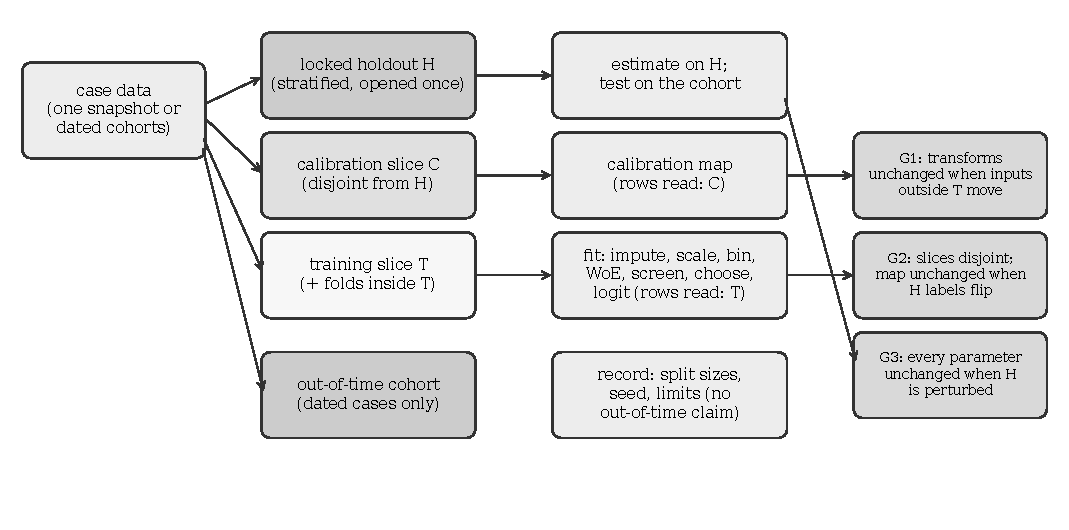
\includegraphics[width=0.95\textwidth]{figures/fig-protocol.pdf}
\caption{The data flow of the protocol for one case: the data are split once into a locked holdout, a calibration slice and a training slice (and, for dated cases, an out-of-time cohort); each fitting step reads only the rows of its slice, and the three gates perturb the rows outside the training slice and require every fitted parameter to be unchanged.}
\label{fig:protocol}
\end{figure}

\subsection{The split declared per case}

The case declares the partition~\eqref{eq:partition} before it fits anything. For the cases that have a single snapshot, the product's split stage draws a locked stratified holdout of 30\% of the rows, then a calibration slice of 20\% of the remaining development rows, stratified on the outcome in both draws, and repeated stratified five-fold cross-validation, twice, inside the training slice for every choice that a rung makes: the number of bins, the penalty, the number of boosting rounds. The split is a pure function of the labels and the seed. With the fractions of the product the slices have the sizes
\begin{equation}
|H|=0.30\,n,\qquad |C|=0.20\,(1-0.30)\,n=0.14\,n,\qquad |T|=0.80\,(1-0.30)\,n=0.56\,n,
\label{eq:sizes}
\end{equation}
up to the rounding of each stratum, so that the card-holder case of Table~\ref{tab:splits} has 9,000, 4,200 and 16,800 rows in 30,000, and the repeated folds inside $T$ divide the training slice without touching the other two. The rules that the split enforces are six and come from the research behind the product: every feature is computed from information available at the observation date; binning, weight of evidence, imputation, scaling and feature selection are fitted on the training slice only; calibration maps are fitted on the calibration slice and never on the test slice; no resampling is applied before calibration is measured; the training set of a loss-given-default or conversion model contains only defaults whose workout window closed before the training cut-off; and macroeconomic covariates enter with the lag that would have been available in real time. The first, fifth and sixth rules are conditions on the data and are enforced by the case that builds them. The second to fourth are conditions on the row sets of equation~\eqref{eq:leakfree}, and they are the ones that the gates test.

The artifact of each case states the sizes of the three slices, their numbers of events, the seed, and the claim that the case makes about the future. Table~\ref{tab:splits} lists what the committed documents of the cases declare: the card-holder case uses one locked holdout and one calibration slice and makes no out-of-time claim because the file is a single snapshot; the corporate bankruptcy files carry no date and the five horizons are five independent samples, so they make none either; the loan case defines five out-of-time cohorts. A case that cannot test the future says so in its artifact instead of leaving the reader to infer it.

\begin{table*}[htbp]
\centering
\small
\caption{The split each case declares in its committed documents: the locked stratified holdout and the disjoint calibration slice of C01 and C02 (the events are those of the holdout) and the out-of-time training windows of C03 (the events are the window's 5-year charge-offs), with the out-of-time claim each case makes or declines to make.}
\label{tab:splits}
\fitwidth{%
\begin{tabular}{llrrl}
\toprule
Case & Split declared in the artifact & Training / calibration / holdout rows & Events & Out-of-time claim \\
\midrule
C01 card holders & \relax locked stratified holdout (30\%), calibration slice, training slice & 16,800 / 4,200 / 9,000 & 1,991 & none: single snapshot \\
C02 horizon 1 & locked stratified holdout, calibration map on a separate slice & 3,309 / 828 / 1,773 & 123 & none: files carry no date \\
C02 horizon 2 & locked stratified holdout, calibration map on a separate slice & 5,483 / 1,371 / 2,938 & 155 & none: files carry no date \\
C02 horizon 3 & locked stratified holdout, calibration map on a separate slice & 5,881 / 1,471 / 3,151 & 149 & none: files carry no date \\
C02 horizon 4 & locked stratified holdout, calibration map on a separate slice & 5,696 / 1,425 / 3,052 & 120 & none: files carry no date \\
C02 horizon 5 & locked stratified holdout, calibration map on a separate slice & 3,934 / 984 / 2,109 & 81 & none: files carry no date \\
C03 cohort FY2006-07 & out-of-time cohort at the 5-year mark; window FY1991 to FY2000, outcomes read to 2005-09-30 & 330,682 window loans & 23,320 & yes \\
C03 cohort FY2008-10 & out-of-time cohort at the 5-year mark; window FY1991 to FY2002, outcomes read to 2007-09-30 & 413,083 window loans & 28,393 & yes \\
C03 cohort FY2011-14 & out-of-time cohort at the 5-year mark; window FY1991 to FY2005, outcomes read to 2010-09-30 & 627,594 window loans & 50,614 & yes \\
C03 cohort FY2015-17 & out-of-time cohort at the 5-year mark; window FY1991 to FY2009, outcomes read to 2014-09-30 & 900,254 window loans & 110,349 & yes \\
C03 cohort FY2018-20 & out-of-time cohort at the 5-year mark; window FY1991 to FY2012, outcomes read to 2017-09-30 & 1,024,597 window loans & 115,237 & yes \\
\bottomrule
\end{tabular}%
}
\end{table*}


\subsection{The out-of-time rule for dated cases}

When the rows are dated, a random split of the pooled rows puts rows of a later vintage into the training slice and rows of an earlier vintage into the holdout, so the estimate on the holdout does not measure the model as it would be used. The protocol replaces the random holdout by a cohort. Let the fiscal years be indexed by their closing year, let a loan approved in fiscal year $f$ have its outcome read $h=5$ years after the end of that year, and let a cohort $c$ begin at fiscal year $g_c$, that is on the first day of the fiscal year that follows $g_c-1$. The training window of the cohort is
\begin{equation}
W_c=\{i:\ f_i\le f_c\},\qquad f_c=\max\{f:\ f+h\le g_c-1\},
\label{eq:window}
\end{equation}
so that the closing date of every outcome in the window precedes the first observation date of the cohort (assumption A4), and the cohort is scored at the 5-year mark of each of its vintages whose mark has passed. The window of the cohort that begins in fiscal year 2015 is fiscal years 1991 to 2009, with outcomes read up to 2014-09-30, and the rule is checked in code before a model is fitted, so that a window that violates it stops the case. The calibration slice of the case is a draw inside the window, disjoint from the rows that the fit used.

\subsection{The three gates and the non-vacuity control}

The gates test the fitting path by perturbation, in the manner of a metamorphic test \citep{chen2018,segura2016}. Let $\Pi_J$ be the perturbation of the rows $J$ that replaces every input by an independent draw from $\mathcal N(5,4^2)$, far outside the range of a standardised input, and every label by a fair coin:
\begin{equation}
\Pi_J(D):\quad x_{ik}\leftarrow\xi_{ik}\sim\mathcal N(5,4^2),\quad y_i\leftarrow\beta_i\sim\mathrm{Bernoulli}(\tfrac12),\qquad i\in J.
\label{eq:perturb}
\end{equation}
Write $\Pi^{X}_J$ for the perturbation of the inputs only and $\theta^{\mathrm{tr}}$ for the parameters of every step before the calibration map, $\kappa$ for the calibration map. The three gates are G1, transforms on the training slice only; G2, a calibration slice disjoint from the test slice; and G3, outside-information invariance:
\begin{align}
\mathrm{G1}:&\quad \theta^{\mathrm{tr}}\bigl(\Pi^{X}_{[n]\setminus T}(D)\bigr)=\theta^{\mathrm{tr}}(D),\label{eq:g1}\\
\mathrm{G2}:&\quad C\cap H=\emptyset\ \wedge\ \kappa\bigl(D^{y_H\leftarrow1-y_H}\bigr)=\kappa(D),\label{eq:g2}\\
\mathrm{G3}:&\quad \theta\bigl(\Pi_H(D)\bigr)=\theta(D)\ \text{for each of }d\text{ independent draws.}\label{eq:g3}
\end{align}
Equality is exact, on every array of the fitted parameters; in the product it is the equality of the fitted details of every rung and of the SHA-256 checksum of its checkpoint. The control that keeps the gates from passing vacuously is that the fit must respond to the data that it is allowed to read:
\begin{equation}
\text{N (non-vacuity):}\quad \theta\bigl(D^{y_{J}\leftarrow1-y_{J}}\bigr)\neq\theta(D),\qquad J\subseteq T,\ |J|=100.
\label{eq:nv}
\end{equation}
A pipeline that ignores its labels, or whose fitted parameters are constants, passes G1 to G3 and fails N. The protocol passes when G1, G2, G3 and N all hold,
\begin{equation}
\mathrm{Pass}=\mathrm{G1}\wedge\mathrm{G2}\wedge\mathrm{G3}\wedge\mathrm{N},
\label{eq:pass}
\end{equation}
and a failure names the gate and, in the product, stops the case. G1 and G3 catch the leaks through the steps that read rows: a statistic fitted on the pooled rows moves when the inputs outside $T$ move. G2 and G3 catch the leaks through the calibration map: a map fitted on $H$ moves when the labels of $H$ flip. A choice among configurations that is made on the holdout is a leak through the step select, and it is caught by G1 and G3 only with the probability that the perturbation changes the choice (Proposition~\ref{prop:discrete}).

\subsection{Algorithm and cost}

Algorithm~\ref{alg:protocol} states the protocol as a procedure. It runs the fitting path once on the data and once under each perturbation, so that its cost is $4+d$ fits of the whole path, plus the evaluation on $H$, which is done once.
\begin{equation}
\mathrm{cost}=(4+d)\,\mathrm{cost}(\mathcal A)+O(n\log n),
\label{eq:cost}
\end{equation}
where the term in $n\log n$ is the AUC and its variance on $H$. The four fits are the base fit, the fit under G1, the fit under G2 and the fit under N; the $d$ perturbation draws of G3 each need one fit. The value $d=1$ is the product's default and Proposition~\ref{prop:discrete} and Section~\ref{sec:results} show when more draws are needed. Two properties of the procedure matter in practice. The fits are independent of one another, so that they can run in parallel, and each is the ordinary fit of the case on a different copy of the data: nothing in the fitting code is changed, and the only requirement on it is that it is a function of its input data and its seeds (assumption A2). The product stops at the first failing gate, while the experiments of this paper run every gate on every leak, in order to measure each gate separately.

\begin{algorithm}[htbp]
\caption{The leakage-safe protocol for one case.}
\label{alg:protocol}
\begin{algorithmic}[1]
\Require data $D=(X,y)$, the case declaration (split fractions, seed, folds, and for a dated case the cohort and the horizon $h$), the fitting procedure $\mathcal A$, the number of perturbation draws $d$
\Ensure the metrics on $H$, the split and its limits, and the outcome of each gate
\State $(T,C,H)\gets\textsc{Split}(y,\text{seed})$ \Comment{locked stratified holdout, calibration slice, training slice}
\If{the case is dated}
  \State $W_c\gets\{i:\ f_i\le f_c\}$ with $f_c$ from~\eqref{eq:window}; check $\max_{i\in W_c}u_i\le b_c$
\EndIf
\State $\theta\gets\mathcal A(D;\,R_s=T\text{ for }s\ne\text{calibrate},\ R_{\text{calibrate}}=C)$ \Comment{the base fit}
\State $\mathrm{G1}\gets[\theta^{\mathrm{tr}}(\Pi^{X}_{[n]\setminus T}D)=\theta^{\mathrm{tr}}(D)]$
\State $\mathrm{G2}\gets[C\cap H=\emptyset\ \wedge\ \kappa(D^{y_H\leftarrow1-y_H})=\kappa(D)]$
\State $\mathrm{G3}\gets\textbf{true}$
\For{$k=1,\dots,d$}
  \State $\mathrm{G3}\gets\mathrm{G3}\wedge[\theta(\Pi_H^{(k)}D)=\theta(D)]$
\EndFor
\State $\mathrm{N}\gets[\theta(D^{y_J\leftarrow1-y_J})\neq\theta(D)]$ for $J\subseteq T$, $|J|=100$
\If{not ($\mathrm{G1}\wedge\mathrm{G2}\wedge\mathrm{G3}\wedge\mathrm{N}$)}
  \State \textbf{stop} and name the failing gate
\EndIf
\State score the calibrated model on $H$ once: $\hat A_H$, its variance $s^2$, the Brier score and the calibration error
\State \Return the metrics, $|T|,|C|,|H|$, their events, the seed, the cohort claim, and the four outcomes
\end{algorithmic}
\end{algorithm}

\subsection{Parameters and implementation}

The parameters are few and each has a reason. The holdout fraction of 30\% and the calibration fraction of 20\% of the development rows give, for the card-holder data, a holdout of \nv{c01.hold} rows with \nv{c01.holdev} events, enough for an interval on the AUC that is narrow compared with the effects measured in Section~\ref{sec:results}, and a calibration slice of \nv{c01.cal} rows. The perturbation law $\mathcal N(5,4^2)$ puts the perturbed inputs far from the training range of a standardised input, so that a step that fits a range, a median or a quantile edge on pooled rows moves with near certainty (Proposition~\ref{prop:detection}); the coin for the labels makes any step that reads labels move. The 100 labels of the control in the compact pipeline (200 in the product's test) are enough to change a regularised fit. The number of draws $d$ trades cost for power against a discrete choice; $d=1$ is the default and $d=5$ is used in Section~\ref{sec:results} to measure that trade.

The reference implementation is the split stage of the product, \texttt{pipeline/\allowbreak{}stages/\allowbreak{}split.py}, and the three gates are the tests \texttt{test\_\allowbreak{}fitted\_\allowbreak{}transforms\_\allowbreak{}train\_\allowbreak{}only}, \texttt{test\_\allowbreak{}calibration\_\allowbreak{}slice\_\allowbreak{}disjoint} and \texttt{test\_\allowbreak{}outside\_\allowbreak{}information\_\allowbreak{}perturbation\_\allowbreak{}invariance} of \texttt{tests/\allowbreak{}test\_\allowbreak{}leakage.py}, which run the product's whole ladder of seven rungs on a planted data set. The experiments of this paper use a compact pipeline of the same steps, \texttt{experiments/\allowbreak{}leaklab.py}, in which every step takes the row set that it reads, so that a leak is exactly a step that reads rows outside its slice and nothing else changes. The AUC and its variance are those of the engine \texttt{riskvalidation} 1.1.0. Complexity is that of equation~\eqref{eq:cost}: the product's ladder test ran the three conditions of Section~\ref{sec:experimental-design} in \nv{e2.ladder.seconds} seconds on one machine, and the gates of the compact pipeline add $4+d$ fits of a scorecard on 1,500 rows.

\section{Theory}
\label{sec:theory}

The propositions of this section state why the protocol should work and under which conditions; each is checked numerically in Section~\ref{sec:results}, and the conditions under which it fails are stated with it. Proposition~\ref{prop:unbiased} says what the holdout estimate is when no step read the holdout. Propositions~\ref{prop:detection} and~\ref{prop:discrete} say with what probability the third gate detects a leak through a quantile edge and through a discrete choice. Proposition~\ref{prop:selection} bounds the optimism of a choice made on the holdout. Propositions~\ref{prop:leakauc} and~\ref{prop:psi} describe a leak that exists only in development and explain what the stability index sees of it. The scaling of the cross-validation bias is stated as a conjecture.

\subsection{The holdout estimate when no step read the holdout}

\begin{proposition}[Unbiasedness]
\label{prop:unbiased}
Let $\theta=\mathcal A(D_R)$ with $R\cap H=\emptyset$, and let the rows of $H$ be an independent sample from the population, independent of $D_R$, with $n_1\ge1$ events and $n_0\ge1$ non-events. Then, conditionally on $\theta$ and on the labels of $H$, the holdout statistic of equation~\eqref{eq:auchat} satisfies $\E[\hat A_H\mid\theta,y_H]=A^{\ast}(\theta)$. If $s^2$ is the DeLong estimator of the variance of $\hat A_H$, then $(\hat A_H-A^{\ast}(\theta))/s$ converges in distribution to $\mathcal N(0,1)$ as $n_1,n_0\to\infty$, and the interval $\hat A_H\pm1.96\,s$ has asymptotic coverage $0.95$.
\end{proposition}
\begin{proof}
Given $\theta$, the score function $S_\theta$ is fixed. Given the labels of $H$, the inputs of the events are independent draws from the distribution of $X$ given $y=1$ and those of the non-events from that given $y=0$, independent of each other. For one event $i$ and one non-event $j$ the kernel $\psi_{ij}=\indic\{S_\theta(x_i)>S_\theta(x_j)\}+\frac12\indic\{S_\theta(x_i)=S_\theta(x_j)\}$ has expectation $A^{\ast}(\theta)$ by equation~\eqref{eq:aucstar}. The statistic $\hat A_H$ is the average of $\psi_{ij}$ over the $n_1n_0$ pairs, so its conditional expectation is $A^{\ast}(\theta)$. It is a two-sample $U$-statistic with a bounded kernel, whose asymptotic normality and whose consistent variance estimator by structural components are the results behind the DeLong interval \citep{delong1988,hanley1982}.
\end{proof}
The proposition fails exactly when $R\cap H\neq\emptyset$: then $\theta$ is a function of the rows of $H$, the pairs are no longer independent of $S_\theta$, and the conditional expectation of the statistic is no longer $A^{\ast}(\theta)$. The sign of the resulting bias is not determined by the proposition; for a procedure that adapts to the rows it reads, it is positive, and Section~\ref{sec:results} measures its size for nine ways of reading the holdout. The proposition also fails when assumption A1 fails: a holdout from a later vintage estimates the performance on that vintage, not on the population of the training rows.

\subsection{Detection by the outside-information gate}

\begin{proposition}[Detection of a leak through a quantile edge]
\label{prop:detection}
Let a step fit the quantile edge at level $q$ of $N$ pooled, continuous, exchangeable values, with $(N-1)q$ not an integer, by linear interpolation between the order statistics of ranks $k-1$ and $k$ with $k=\lfloor(N-1)q\rfloor+2$, and let this edge be read from a pool that contains $m$ outside rows. Let the third gate send these $m$ rows above the maximum of the pool, the $m$ rows being a uniformly random subset of the $N$ pooled rows. Then the edge changes unless every moved row has rank above $k$ in the pool, and
\begin{equation}
\begin{split}
\Prob(\text{gate detects})&=1-\frac{\binom{N-k}{m}}{\binom{N}{m}}\\
&\ge\ 1-(1-q)^m .
\end{split}
\label{eq:detect}
\end{equation}
\end{proposition}
\begin{proof}
The order statistic of rank $j\le N-m$ of the perturbed pool is the $j$-th smallest of the $N-m$ rows that were not moved. It equals the original order statistic of rank $j$ if and only if no moved row has original rank at most $j$. The edge is a function of the order statistics of ranks $k-1$ and $k$, so it is unchanged if no moved row has rank at most $k$; if a moved row has rank $r\le k$, every order statistic of rank $j\ge r$ is replaced by a strictly larger value, in particular the one of rank $k$, and its weight in the interpolation, $(N-1)q-\lfloor(N-1)q\rfloor$, is positive, so the edge changes. The moved set is a uniformly random $m$-subset of the ranks, so the probability that all its elements lie among the $N-k$ ranks above $k$ is $\binom{N-k}{m}/\binom{N}{m}=\prod_{j=0}^{m-1}\frac{N-k-j}{N-j}$. Each factor is at most $\frac{N-k}{N}$, and $k\ge(N-1)q+1$ gives $\frac{N-k}{N}\le\frac{(N-1)(1-q)}{N}<1-q$.
\end{proof}
For the pool of the experiments, $N=\nv{th.det.ntrain}+\nv{th.det.nout}$ pools the development rows (the training and the calibration slices) and the holdout rows and $q=0.9$, so that $k=1351$, the probability that one moved row is detected is $\nv{th.det.1.exact}\%$ and that two are detected is $\nv{th.det.2.exact}\%$. The gate that moves the whole holdout, $m=|H|=450$, cannot miss, since $m$ exceeds $N-k=149$ and the probability of the proposition is exactly zero, so that the detection of a leak through a step that fits an edge on pooled rows does not depend on the gate but on whether the step reads the rows at all. A step that fits a median or a mean has the same property with $q=\frac12$ or, for a mean, with certainty.

\subsection{Optimism of a choice made on the holdout}

\begin{proposition}[Selection on the holdout]
\label{prop:selection}
Let $K$ configurations have true values $a_k=A^{\ast}(\theta_k)$ and holdout estimates $\hat A_k=a_k+Z_k$, where each $Z_k$ is sub-Gaussian with variance proxy $\sigma^2$, that is $\E e^{\lambda Z_k}\le e^{\lambda^2\sigma^2/2}$. Let $\hat k=\arg\max_k\hat A_k$. Then
\begin{equation}
\E\bigl[\hat A_{\hat k}-a_{\hat k}\bigr]\ \le\ \sigma\sqrt{2\ln K}.
\label{eq:selectbound}
\end{equation}
For the Mann-Whitney statistic of equation~\eqref{eq:auchat} one may take $\sigma^2=1/(4\min(n_1,n_0))$.
\end{proposition}
\begin{proof}
$\hat A_{\hat k}-a_{\hat k}=Z_{\hat k}\le\max_kZ_k$. For $\lambda>0$, Jensen's inequality gives $\E\max_kZ_k\le\frac1\lambda\ln\E\sum_ke^{\lambda Z_k}\le\frac{\ln K}{\lambda}+\frac{\lambda\sigma^2}{2}$, and the choice $\lambda=\sqrt{2\ln K}/\sigma$ gives the bound. The statistic $\hat A_H$ is a two-sample $U$-statistic with a kernel in $[0,1]$; Hoeffding's representation of it as an average of means of $\min(n_1,n_0)$ independent pairs and the convexity of the exponential give $\E\exp\{\lambda(\hat A_H-\E\hat A_H)\}\le\exp\{\lambda^2/(8\min(n_1,n_0))\}$, which is the condition on $Z_k$ with $\sigma^2=1/(4\min(n_1,n_0))$ \citep{hoeffding1963,boucheron2013}.
\end{proof}
The bound is for the worst case, in which the estimates are independent. Configurations of one pipeline are strongly dependent, and the maximum of $K$ standard normal variables with pairwise correlation $\rho$ has a mean of $\nv{th.max.8.r0.0}$ for $K=8$ at $\rho=0$, $\nv{th.max.8.r0.5}$ at $\rho=0.5$ and $\nv{th.max.8.r0.9}$ at $\rho=0.9$, in units of $\sigma$, against the bound $\nv{th.max.8.bound}$ (simulation with 20,000 draws per cell, the correlation induced by a common factor). The optimism of a choice made on the holdout is therefore small when the configurations are similar and grows with $\sqrt{\ln K}$ when they are not, which is the pattern of Section~\ref{sec:results}.

\subsection{A leak that exists only in development}

The planted leak of the engine's generator is the case in which a feature carries the outcome in development and is noise at decision time. Let the score be $S=w_1G+w_2F$, where $G\sim\mathcal N(d\,y,1)$ is the genuine feature and $F$ an independent feature that is $\mathcal N(s\,y,1)$ in development and $\mathcal N(0,1)$ at decision time.

\begin{proposition}[AUC of a score with a planted leak]
\label{prop:leakauc}
In development, and at decision time, the AUC of $S$ is
\begin{equation}
\AUC_{\mathrm{dev}}=\Phi\!\left(\frac{w_1d+w_2s}{\sqrt{2(w_1^2+w_2^2)}}\right),\qquad
\AUC_{\mathrm{cur}}=\Phi\!\left(\frac{w_1d}{\sqrt{2(w_1^2+w_2^2)}}\right),
\label{eq:leakauc}
\end{equation}
where $\Phi$ is the standard normal distribution function. The development AUC is largest for $w\propto(d,s)$, where it equals $\Phi\bigl(\sqrt{(d^2+s^2)/2}\bigr)$, and the decision-time AUC of that score is $\Phi\bigl(d^2/\sqrt{2(d^2+s^2)}\bigr)$, which is below the AUC $\Phi(d/\sqrt2)$ of the genuine feature alone whenever $s>0$. For equal weights, $\AUC_{\mathrm{dev}}=\Phi((d+s)/2)$ and $\AUC_{\mathrm{cur}}=\Phi(d/2)$.
\end{proposition}
\begin{proof}
The score difference $S_1-S_0$ between a defaulter and a survivor is normal with mean $w_1d+w_2s$ in development, $w_1d$ at decision time, and variance $2(w_1^2+w_2^2)$, so the AUC $\Prob(S_1-S_0>0)$ is $\Phi(\mu/\sqrt{2(w_1^2+w_2^2)})$ with the mean $\mu$ of the case. By the Cauchy-Schwarz inequality $w_1d+w_2s\le\sqrt{d^2+s^2}\sqrt{w_1^2+w_2^2}$, with equality at $w\propto(d,s)$, which gives the maximum; substituting $w_1/\sqrt{w_1^2+w_2^2}=d/\sqrt{d^2+s^2}$ gives the decision-time AUC. The AUC of the genuine feature alone is the case $w_2=0$. The comparison follows from $d/\sqrt{d^2+s^2}<1$.
\end{proof}
At $d=1$ and $s=1$ with equal weights, the development AUC is $\Phi(1)=\nv{e3.s1.0.devcf}$ and the decision-time AUC $\Phi(\tfrac12)=\nv{e3.s1.0.curcf}$: the leak inflates the development AUC by $\nv{e3.s1.0.infl}$, and the model is worse at decision time than the genuine feature alone, whose AUC is $\Phi(1/\sqrt2)=\nv{th.opt.1.0.clean}$. The test that compares the current AUC with its development value sees the whole gap. The index that compares the distribution of the leaked feature between development and a reference sees a much smaller quantity.

\begin{proposition}[Stability index of the leaked feature]
\label{prop:psi}
Let the leaked feature be $\mathcal N(0,1)$ for survivors and $\mathcal N(s,1)$ for the share $\pi$ of defaulters, and let the reference sample be $\mathcal N(0,1)$. For a binning with reference probabilities $p_b$ and defaulter probabilities $r_b=\Phi(e_b-s)-\Phi(e_{b-1}-s)$, the population stability index of the mixture is
\begin{equation}
\mathrm{PSI}=\pi^2\sum_b\frac{(r_b-p_b)^2}{p_b}+O(\pi^3),\qquad\text{and, for fine bins, }\ \mathrm{PSI}\approx\pi^2\bigl(e^{s^2}-1\bigr).
\label{eq:psi}
\end{equation}
\end{proposition}
\begin{proof}
The mixture has bin probabilities $m_b=p_b+\pi(r_b-p_b)$. With $x_b=\pi(r_b-p_b)/p_b$ the index is $\sum_b(m_b-p_b)\ln(m_b/p_b)=\sum_bp_bx_b\ln(1+x_b)=\sum_bp_b\bigl(x_b^2-\tfrac12x_b^3+\dots\bigr)$, and the quadratic term is the first term of~\eqref{eq:psi}. For fine bins $\sum_b(r_b-p_b)^2/p_b$ tends to the chi-square divergence between $\mathcal N(s,1)$ and $\mathcal N(0,1)$, which is $e^{s^2}-1$.
\end{proof}
The index of two samples of 5,000 rows each, binned in ten deciles, has an expectation of $(B-1)(1/5000+1/5000)=\nv{th.psi.null}$ when the two samples agree \citep{yurdakul2020}. With the generator's share $\pi=0.03$ the second-order form gives $\nv{th.psi.1.0.binned_chi2_form}$ at $s=1$, below that level: the leak is invisible to the index. The binned form is within 11\% of the exact index of the engine at every $s$ up to 3 (\nv{th.psi.3.0.binned_chi2_form} against \nv{th.psi.3.0.engine_psi} at $s=3$); the continuous form is within 13\% up to $s=0.5$ and diverges beyond it (\nv{th.psi.3.0.continuous_form} at $s=3$), because the decile grid cannot resolve the tails that the exponential describes. The simulated index under no leak has a mean of \nv{e3.s0.0.psi}, which agrees with the expectation.

\subsection{Detection of a discrete choice by repeated perturbation}

The gates of the protocol perturb the holdout once by default, and a leak that consists in choosing among a few configurations on the holdout leaves a discrete trace in the fitted parameters: the parameters change only when the perturbed holdout makes another configuration the best one. The next proposition gives the detection probability of that trace as a function of the number of perturbation draws.

\begin{proposition}[Detection of a discrete choice]
\label{prop:discrete}
Let a leak consist in choosing one of $K$ configurations by the highest score on $H$, and let the perturbation of $H$ be such that the choice that would be made on the perturbed holdout is uniformly distributed on the $K$ configurations, independently across $d$ independent perturbation draws. Then the third gate fails, for the base choice, with probability $1-K^{-d}$.
\end{proposition}
\begin{proof}
A draw does not change the choice with probability $1/K$, because the perturbed choice is uniform and equals the base choice with that probability. The draws are independent, so the choice survives all $d$ draws with probability $K^{-d}$.
\end{proof}
Uniformity is the condition. When the labels of $H$ are redrawn at random the scores of the configurations on $H$ are exchangeable if the configurations are similar models, and the proposition applies; when one configuration dominates for structural reasons, the perturbed choice equals the base choice more often than $1/K$ and the detection is lower than the proposition states. The measurement of Section~\ref{sec:results} is the check.

\subsection{Scaling of the bias of cross-validation with preprocessing outside the folds}

\begin{conjecture}[Scaling of the cross-validation bias]
\label{conj:cv}
For a scorecard whose binning, weight of evidence and screening of the best $k$ of $p$ inputs are fitted on all development rows before the folds, the bias of the five-fold AUC against the AUC of the fold models has the form $b(n,p)\approx c(p)\,n^{-\alpha}$ with $\alpha$ between $0.8$ and $1$, and $c(p)$ increasing and concave in $p$.
\end{conjecture}
The heuristic is that the optimism of an in-sample AUC grows with the effective number of fitted parameters divided by $n$, which gives $\alpha=1$, and that the screening of the best ten inputs among $p$ adds an optimism that grows with $p$ but saturates once the ten best noise inputs are essentially the extreme order statistics. The evidence is Table~\ref{tab:cv-scaling}: a log-log regression over $n=400$ to $6{,}400$ at $p=40$ gives a slope of $-\nv{e5.exp}\pm\nv{e5.expse}$ (standard error), and at $n=1{,}600$ the bias moves from \nv{e5.n1600.p10.out} at 10 inputs to \nv{e5.n1600.p160.out} at 160. The slope is below one in magnitude by more than ten standard errors, so the conjecture is stated with $\alpha<1$; the concavity in $p$ is read from five points and is weak evidence. The range of $\alpha$ between 0.8 and 1 was read from this same fit, so that the experiment describes the conjecture and does not test it; a test needs data sets or cells that were not used to state it. The conjecture is not proved, and it is stated for the scorecard of the experiments, whose informative inputs are five of $p$.

\section{Experimental design}
\label{sec:experimental-design}

The experiments measure two things about the protocol of Section~\ref{sec:proposed-method}: what each way of breaking it costs in the validation estimate, and what each gate sees. Every comparison is paired: the protocol and each leaked variant are fitted on the same data draw with the same seed, so that a difference between them is the effect of the row set that one step read and nothing else.

\subsection{Predictions}

Nine predictions are fixed, each with a decision rule in terms of a measured quantity applied by the table script to the cells of the paper that the prediction names (the caption of Table~\ref{tab:hypotheses} lists them; H1, H2 and H4 include the product's own scorecard, which the paper reports with the protocol, with the fit on every row and with the calibration map), and a prediction that fails is reported as not held. They were not stated before the results and were not registered outside the repository: the author wrote them in the table script between 4 and 7 November 2026, during the analysis (the record does not date the writing more closely), together with the experiment outputs that decide them, and the outputs were committed with them. For two of them the record shows that part of the answer was already known. The committed document of the case C22 (31 October 2026) held an AUC-test power of \nv{c22.auc.0.5}\% at $s=0.5$ and a stability-index power of \nv{c22.csi.1}\% at $s=1$, and H6 asks for at least 97\% and at most 20\%; the committed documents of the case C03 (30 October 2026) held out-of-time gaps of the scorecard whose smallest absolute value is \nv{c03.mingap} points, and H8 asks for at least 2. H6 and H8 are therefore checks that new runs reproduce committed values against thresholds placed beside them, not tests of an unseen outcome. For the other seven the record shows no earlier statement, and none is claimed. Table~\ref{tab:hypotheses} gives them with the quantity that decides each and its outcome, which the table script computes from the committed outputs of the experiments by the rule written in the prediction; no outcome is entered by hand. The predictions cover the unbiasedness of the protocol (H1), the direction and size of the bias of the leaks that read holdout labels (H2), the steps that read only holdout inputs (H3), the calibration map (H4), the detection by the gates (H5), the leak that exists only in development (H6), the closed forms of the theory (H7), the random split against the out-of-time cohort (H8) and cross-validation (H9). The thresholds (0.005 for a negligible bias; 97\%, 20\% and 2\% for the power of the three detectors of the planted leak; 1 and 2 percentage points for the level gap) are the decision rules of the design, round values chosen by the author; no proposition predicts the 97\%, 20\% or 2\% levels. The table gives the measured quantity next to each outcome so that a reader can apply other thresholds.

\begin{table*}[htbp]
\centering
\small
\caption{The nine predictions of the experimental design, each with the quantity that decides it and its outcome, computed by the table script from the committed experiment outputs. A prediction that fails is reported as not held.}
\label{tab:hypotheses}
\fitwidth{%
\begin{tabular}{lp{7.2cm}p{4.6cm}l}
\toprule
Id & Prediction stated before the experiments & Evidence & Outcome \\
\midrule
H1 & \relax The proposed protocol's holdout AUC is unbiased for the fitted model's true AUC (the 95\% interval of the bias contains 0) and its 95\% interval covers (the Wilson interval of the coverage contains 0.95); refuted if either fails in any cell. & 6 of 6 cells & held \\
H2 & \relax A step that reads holdout labels (WoE, screen, or the whole fit) inflates the AUC (the 95\% interval of the bias excludes 0 from above); refuted if any of the three does not in a data set. & syn: 3 of 3, small: 3 of 3, tw: 2 of 3 & not held \\
H3 & A step that reads only holdout inputs (imputation, scaling, bin edges) leaves the estimate within 0.005 of the truth. & 12 of 12 cells & held \\
H4 & A calibration map fitted on the holdout biases the AUC and the Brier score optimistically (positive AUC bias, negative Brier bias, intervals excluding 0). & 6 of 6 cells & held \\
H5 & At least one of the three gates fails on every leak planted in the fitting path, in every draw, and none fails on the proposed protocol. & \relax 15 of 15 leaks, false alarms 0\% & held \\
H6 & \relax A leak that exists only in development is flagged by the AUC-against-development test (power at least 97\% at s = 0.5) and not by the CSI of the leaked feature (power at most 20\% at s = 1) or the single-feature screen (at most 2\% at s = 1). & \relax AUC test power 99.0\% at s = 0.5; CSI power 14.2\% and single-feature flag 0.0\% at s = 1 & held \\
H7 & The closed forms of Proposition 4 reproduce the generator's exact development and decision-time AUC and the simulated means within three standard errors. & largest absolute z 1.8 over seven levels & held \\
H8 & A random split inside the training window reports a level gap below 1 point for every cohort, while the out-of-time gap is at least 2 points. & random gap below 1 point in 5 of 5 cohorts; out-of-time gap at least 2 points in 5 of 5 & held \\
H9 & Preprocessing fitted before the folds inflates the cross-validated AUC; fitted inside the folds it does not. & outside-fold bias positive, inside-fold bias null & held \\
\bottomrule
\end{tabular}%
}
\end{table*}


\subsection{Data and their provenance}

\paragraph{Planted data.} The planted data have a known truth. Each row has $p=40$ independent standard normal inputs, five of which are informative with coefficients $(0.9,-0.7,0.6,0.5,-0.4)$ in a logistic model with intercept $-1.3$, so that the event share is \nv{syn.share}\% and the true probability of every row is known; 5\% of the values in ten of the inputs are set missing completely at random. The development sample has \nv{syn.n} rows (and \nv{small.n} rows in the small-sample variant); the split gives a holdout of \nv{syn.hold} rows. A reference sample of \nv{syn.oracle} rows is drawn from the same model in every repetition, and no step reads it. The reference AUC of a fitted model on this sample has a sampling error of \nv{syn.orcse} (Hanley and McNeil standard error), which is mean-zero across repetitions and does not bias the comparison.

\paragraph{Card holders (C01).} The UCI data set of 30,000 credit-card clients in Taiwan, with the default of the next month as outcome, a share of \nv{c01.rate}\% \citep{yeh2009}; the data are distributed under CC BY 4.0 (\url{https://doi.org/10.24432/C55S3H}). Each repetition draws \nv{tw.oracle} rows as the reference sample and \nv{tw.n} other rows as the development sample, using the \nv{tw.p} numeric inputs of the case. The reference sample has a sampling error of \nv{tw.orcse} in the AUC, larger than that of the planted data, which makes the coverage of the interval on this data set slightly understated and leaves the bias unchanged.

\paragraph{SBA 7(a) loans (C03).} The 7(a) loan files of the U.S. Small Business Administration (\url{https://data.sba.gov/dataset/7a-504-foia}, licence ``U.S. Government Works'', files dated 30 June 2026 in their names), with the 5-year charge-off as outcome, in five cohorts of approval fiscal years whose training windows follow equation~\eqref{eq:window}; Table~\ref{tab:splits} gives the windows. The product's fit of the window and the scorecard and gradient-boosting rungs are the ones of the case, with the seed of the committed documents; the experiment reproduces the committed out-of-time AUC of the scorecard to within \nv{e4.maxrepdiff} for every cohort.

\paragraph{The engine's planted leak (C22).} The binormal generator of the engine \texttt{riskvalidation} 1.1.0 with 150 defaulters and 4,850 survivors in each of the development and the current sample, a genuine score with separation $d=1$, and a leaked feature that is shifted by $s\in\{0,0.25,0.5,1,1.5,2,3\}$ standard deviations for defaulters in development and is noise at decision time. The committed document of the case holds the exact truth of the generator at six of these levels, and the closed forms of Proposition~\ref{prop:leakauc} reproduce it.

\paragraph{The product's scorecard and ladder.} The product's own optbinning scorecard \citep{navas2020} with monotone binning, information-value screen and sign check, fitted on planted data with 12 inputs, and the product's whole ladder of seven rungs, on a planted set of \nv{e2.ladder.n} rows.

\subsection{Methods compared}

The published practices are run, not quoted. Each is a variant of the compact pipeline of Section~\ref{sec:proposed-method} in which one step reads the holdout, so that it is the practice that the cited work describes and nothing else. Imputation and scaling on all development and holdout rows is the pooled preprocessing that the standard textbooks warn against \citep{hastie2009,moscovich2022}. Bin edges on all rows is the same for the supervised binning of a scorecard \citep{siddiqi2017}. The weight of evidence and the association screen computed with the holdout labels are the selection bias of Ambroise and McLachlan \citep{ambroise2002}. Everything fitted on training and holdout is the model whose holdout is its own training data. The configuration chosen on the holdout is the practice of choosing the candidate by the validation AUC and reporting the AUC on the same partition \citep{cawley2010,autobayesian2026}. The calibration map fitted on the holdout, and a calibration slice that overlaps the holdout by 20\% of its rows, are the faulty uses of the held-out data that calibration requires \citep{niculescu2005,zadrozny2002}. Two five-fold procedures complete the set: preprocessing inside each training fold and preprocessing on all development rows before the folds \citep{ambroise2002,varma2006}. The detectors of the planted leak are the engine's own: the ECB discrimination test of the current AUC against the development AUC, with the exact development AUC of the generator passed as the known development value, which is the reading of the ECB instructions \citep{ecb2019}, the characteristic stability index of the leaked feature \citep{yurdakul2020}, the single-feature AUC screen with its threshold of 0.95, and the resemblance AUC between the development and the current feature, the engine's implementation of the idea of the sample-similarity tests of the open toolkits \citep{mercury2023,probatus2026}. The toolkits themselves are not run (Section~\ref{sec:limitations}).

\subsection{Metrics}

The bias of the holdout AUC, the Brier score and the expected calibration error is the mean over repetitions $r=1,\dots,R$ of the estimate on $H$ minus the value of the same fitted model on the reference sample,
\begin{equation}
\hat b=\frac1R\sum_{r=1}^R\Bigl(\hat A_H^{(r)}-\hat A_{\mathrm{ref}}^{(r)}\Bigr),\qquad
\mathrm{se}(\hat b)=\frac{\mathrm{sd}_r\bigl(\hat A_H^{(r)}-\hat A_{\mathrm{ref}}^{(r)}\bigr)}{\sqrt R},
\label{eq:biashat}
\end{equation}
reported as $\hat b\pm1.96\,\mathrm{se}(\hat b)$, with the root mean squared error $\bigl(\frac1R\sum_r(\hat A_H^{(r)}-\hat A_{\mathrm{ref}}^{(r)})^2\bigr)^{1/2}$. The Brier score is $\frac1{|H|}\sum_{i\in H}(\hat p_i-y_i)^2$ and the calibration error is
\begin{equation}
\mathrm{ECE}=\sum_{g=1}^{10}\frac{|H_g|}{|H|}\,\bigl|\bar p_g-\bar y_g\bigr|,
\label{eq:ece}
\end{equation}
over ten groups of equal size of the predicted probability. The coverage of the engine's interval is the share of repetitions with $|\hat A_H-\hat A_{\mathrm{ref}}|\le1.96\,s$, with its Wilson interval \citep{brown2001}. The detection rate of a gate or a test is the share of draws in which it rejects, with a Wilson interval. For the out-of-time comparison the gap is the observed minus the predicted 5-year rate,
\begin{equation}
\mathrm{gap}=\bar y-\bar p,
\label{eq:gap}
\end{equation}
in percentage points, and the AUC is that of the same fitted rungs on the two samples. A closed form of the theory is checked by the standardised difference
\begin{equation}
z=\frac{\hat\mu_{\mathrm{sim}}-\mu_{\mathrm{formula}}}{\mathrm{se}(\hat\mu_{\mathrm{sim}})},
\label{eq:zscore}
\end{equation}
which has to stay within three for the formula to be accepted. These choices follow the practice for simulation studies \citep{morris2019}.

\subsection{Protocol, repetitions and seeds}

Table~\ref{tab:design} lists the experiments, their data, repetitions and seeds. Every repetition has its own seed, derived from the experiment seed and the repetition number by a seed sequence, so that a repetition can be rerun alone and the results do not depend on the number of workers. The statistics are those of the metrics above: 95\% half-widths over repetitions, Wilson intervals for proportions, and the standardised difference for the closed forms. The number of repetitions follows from the resolution that the comparisons need: a half-width of 0.002 in the AUC bias on 2,500 rows separates the leaks that cost more than 0.004 from the protocol, and 100 draws of the gates give a Wilson upper bound of \nv{e2.fa.upper}\% for the false-alarm rate when none occurs. The out-of-time experiment has one fit per cohort, since the longest cohort took \nv{run.e4max} seconds, and its uncertainty is the binomial error of the 5-year rates.

\begin{table}[htbp]
\centering
\small
\caption{The experiments, the data each runs on, the number of repetitions and the seed; every repetition draws its own data, split and reference sample from the seed of the experiment and its own index, and all variants of one repetition share the draw.}
\label{tab:design}
\fitwidth{%
\begin{tabular}{llrr}
\toprule
Experiment & Data and what varies & Repetitions & Seed \\
\midrule
Bias of the estimate & planted, \nv{syn.n} rows, nine leaks and two five-fold procedures & \nv{syn.reps} & \nv{syn.seed} \\
 & planted, \nv{small.n} rows & \nv{small.reps} & \nv{small.seed} \\
 & card holders, \nv{tw.n} rows from 30,000 & \nv{tw.reps} & \nv{tw.seed} \\
 & product scorecard, 12 inputs, two leaks & \nv{prod.reps} & \nv{prod.seed} \\
Gates & planted, \nv{e2.n} rows, every leak, three gates and the control & \nv{e2.reps} & 20261108 \\
 & discrete choice, one to five perturbation draws & \nv{e2.draws.reps} & 20261108 \\
Planted leak & engine generator, seven leak levels, four detectors & \nv{e3.reps} & 20261109 \\
Closed forms & Propositions~\ref{prop:detection}, \ref{prop:selection}, \ref{prop:leakauc} and \ref{prop:psi} & 10,000 to 20,000 & 20261110 \\
Cross-validation & planted, nine combinations of rows and inputs & \nv{e5.reps} & 20261111 \\
Out-of-time & SBA loans, five cohorts, one fit per cohort & 1 & 42 \\
\bottomrule
\end{tabular}%
}
\end{table}

\subsection{Ablations planned}

Two ablations are planned and reported in Section~\ref{sec:ablation}. The first removes one component of the protocol at a time (statistics fitted on the training slice only, configuration chosen inside the training slice, calibration on a slice disjoint from the test slice, preprocessing inside the folds) and reads the cost from the bias and the coverage of the corresponding leak. The second keeps every subset of the three gates and reads, for the leaks planted in the fitting path, the number that at least one gate of the subset detects in every draw, the number that no gate of the subset detects, the mean detection and the false-alarm rate on the protocol. In both ablations the comparison is paired, with the protocol on the same draws as the reference. The first ablation takes, for each rule, the worst leak that its removal allows, so that a rule that is cheap to remove under one leak is not credited with the cost of another; the second reports the share of draws in which a subset detects and not a single threshold, so that a reader can set the level of detection that a pipeline requires.

\section{Results}
\label{sec:results}

\subsection{The bias of the holdout estimate}

Table~\ref{tab:main-results} gives the main comparison. Under the protocol the holdout AUC of the WoE scorecard has a bias of \nv{syn.w.none.bias}$\,\pm\,$\nv{syn.w.none.ci} against the reference sample, a root mean squared error of \nv{syn.w.none.rmse}, and the 95\% interval of the engine covers the reference value in \nv{syn.w.none.cov}\% of the \nv{syn.reps} repetitions (Wilson interval \nv{syn.w.none.covlo} to \nv{syn.w.none.covhi}\%). The standardised logit has a bias of \nv{syn.l.none.bias}$\,\pm\,$\nv{syn.l.none.ci} and a coverage of \nv{syn.l.none.cov}\%. The same holds in the other three settings of Table~\ref{tab:other-data}: on \nv{small.n} rows the bias is \nv{small.w.none.bias}$\,\pm\,$\nv{small.w.none.ci} with a coverage of \nv{small.w.none.cov}\%, on the card holders \nv{tw.w.none.bias}$\,\pm\,$\nv{tw.w.none.ci} with \nv{tw.w.none.cov}\%, and for the product's own scorecard \nv{prod.p.none.bias}$\,\pm\,$\nv{prod.p.none.ci} with \nv{prod.p.none.cov}\% (Wilson interval \nv{prod.p.none.covlo} to \nv{prod.p.none.covhi}\%). In all six cells of the two models and three data sets the interval of the bias contains zero and the interval of the coverage contains 0.95, so that the first prediction holds and Proposition~\ref{prop:unbiased} is borne out. The calibration error is the exception: its bias under the protocol is \nv{syn.w.none.ece} for the scorecard, because the average of the absolute differences over ten groups of 75 rows is positive even for a perfectly calibrated model, while the reference rows, 50,000 of them, make it nearly zero; it is a property of the estimator of the calibration error at this holdout size and not of the protocol. The Brier score has a second small exception: its bias under the protocol is negative on the small sample (\nv{small.w.none.brier}$\,\pm\,$\nv{small.w.none.brierci}) and on the card holders (\nv{tw.w.none.brier}$\,\pm\,$\nv{tw.w.none.brierci}), with an interval that excludes zero, so that the holdout scores a little better than the reference sample. A plausible cause, not tested here, is that the stratified holdout shares the event share on which the intercept of the model was fitted, while each reference sample is drawn afresh; the size is smaller than the Brier effect of the calibration leak (\nv{syn.w.caltest.brier}).

\begin{table*}[htbp]
\centering
\small
\caption{Bias of the holdout estimate of the AUC, the Brier score and the calibration error against the value on a reference sample of 50,000 rows that no step read, for the proposed protocol and for each leaked variant, on 300 planted data sets of 2,500 rows with 40 inputs; the coverage column is the share of the 95\% intervals of the engine's AUC variance that contain the reference value. The two five-fold rows compare the cross-validated AUC with the mean reference AUC of the fold models.}
\label{tab:main-results}
\fitwidth{%
\begin{tabular}{llrrrrr}
\toprule
Model & Validation procedure & AUC bias $\pm$ 95\% half-width & RMSE & Coverage \% [Wilson 95\%] & Brier bias & ECE bias \\
\midrule
WoE scorecard & proposed protocol & $0.000\pm0.002$ & 0.018 & 95.3 [92, 97] & $-0.0001\pm0.0008$ & $+0.0148\pm0.0014$ \\
 & imputation on all rows & $0.000\pm0.002$ & 0.018 & 95.3 [92, 97] & $0.0000\pm0.0008$ & $+0.0145\pm0.0014$ \\
 & bin edges on all rows & $-0.001\pm0.002$ & 0.018 & 96.3 [94, 98] & $+0.0001\pm0.0008$ & $+0.0147\pm0.0014$ \\
 & WoE with holdout labels & $+0.018\pm0.002$ & 0.026 & 78.3 [73, 83] & $-0.0062\pm0.0008$ & $+0.0126\pm0.0014$ \\
 & screen with holdout labels & $+0.004\pm0.002$ & 0.019 & 94.3 [91, 96] & $-0.0016\pm0.0008$ & $+0.0132\pm0.0013$ \\
 & everything fitted on training and holdout & $+0.025\pm0.002$ & 0.032 & 66.7 [61, 72] & $-0.0088\pm0.0009$ & $+0.0113\pm0.0014$ \\
 & configuration chosen on the holdout & $+0.005\pm0.002$ & 0.018 & 96.0 [93, 98] & $-0.0018\pm0.0008$ & $+0.0127\pm0.0013$ \\
 & calibration map fitted on the holdout & $+0.016\pm0.002$ & 0.023 & 88.0 [84, 91] & $-0.0081\pm0.0007$ & $-0.0055\pm0.0011$ \\
 & calibration slice overlapping the holdout & $+0.004\pm0.002$ & 0.018 & 94.3 [91, 96] & $-0.0022\pm0.0008$ & $+0.0113\pm0.0014$ \\
 & five-fold, preprocessing inside the folds & $-0.001\pm0.002$ & 0.015 & -- & -- & -- \\
 & five-fold, preprocessing before the folds & $+0.054\pm0.001$ & 0.055 & -- & -- & -- \\
standardised logit & proposed protocol & $-0.001\pm0.002$ & 0.017 & 94.7 [92, 97] & $+0.0002\pm0.0008$ & $+0.0150\pm0.0012$ \\
 & imputation on all rows & $-0.001\pm0.002$ & 0.017 & 94.3 [91, 96] & $+0.0002\pm0.0008$ & $+0.0142\pm0.0013$ \\
 & scaling on all rows & $-0.001\pm0.002$ & 0.017 & 95.0 [92, 97] & $+0.0002\pm0.0008$ & $+0.0149\pm0.0012$ \\
 & screen with holdout labels & $+0.004\pm0.002$ & 0.017 & 93.7 [90, 96] & $-0.0017\pm0.0008$ & $+0.0130\pm0.0012$ \\
 & everything fitted on training and holdout & $+0.009\pm0.002$ & 0.019 & 92.7 [89, 95] & $-0.0034\pm0.0008$ & $+0.0118\pm0.0013$ \\
 & configuration chosen on the holdout & $-0.001\pm0.002$ & 0.017 & 95.0 [92, 97] & $+0.0002\pm0.0008$ & $+0.0150\pm0.0013$ \\
 & calibration map fitted on the holdout & $+0.014\pm0.002$ & 0.021 & 87.0 [83, 90] & $-0.0079\pm0.0007$ & $-0.0063\pm0.0011$ \\
 & calibration slice overlapping the holdout & $+0.003\pm0.002$ & 0.017 & 96.0 [93, 98] & $-0.0019\pm0.0007$ & $+0.0109\pm0.0012$ \\
 & five-fold, preprocessing inside the folds & $-0.001\pm0.001$ & 0.012 & -- & -- & -- \\
 & five-fold, preprocessing before the folds & $+0.005\pm0.001$ & 0.013 & -- & -- & -- \\
\bottomrule
\end{tabular}%
}
\end{table*}


Figure~\ref{fig:bias-by-leak} shows the AUC bias of every variant with its interval, for both models and two sample sizes. Three groups appear. The first group reads only holdout inputs: imputation on all rows, scaling on all rows and bin edges on all rows. On the planted data their biases are \nv{syn.w.imp.bias} (imputation) and \nv{syn.w.bin.bias} (bin edges) for the scorecard and \nv{syn.l.imp.bias} (imputation) and \nv{syn.l.scale.bias} (scaling) for the logit, all within the half-width of the protocol, and the same holds on the small sample and the card holders, so that the prediction that these steps leave the estimate within 0.005 of the truth holds in all twelve cells. The second group reads holdout labels. The weight of evidence computed with the holdout labels adds \nv{syn.w.woe.bias}$\,\pm\,$\nv{syn.w.woe.ci} to the AUC of the scorecard and lowers the coverage to \nv{syn.w.woe.cov}\%; fitting every step on the training slice and the holdout adds \nv{syn.w.fit.bias}$\,\pm\,$\nv{syn.w.fit.ci}, and the coverage falls to \nv{syn.w.fit.cov}\%. The logit, whose steps are less flexible, gains less: \nv{syn.l.fit.bias} with a coverage of \nv{syn.l.fit.cov}\%. The third group is the calibration: a map fitted on the holdout adds \nv{syn.w.caltest.bias}$\,\pm\,$\nv{syn.w.caltest.ci} to the AUC of the scorecard and \nv{syn.l.caltest.bias} to that of the logit, lowers the Brier score by \nv{syn.w.caltest.brier} and turns the bias of the calibration error from \nv{syn.w.none.ece} to \nv{syn.w.caltest.ece}: the model looks better calibrated than it is, and by a margin that is of the order of the whole error. A calibration slice that overlaps the holdout in a fifth of its rows adds \nv{syn.w.calov.bias} to the AUC, in proportion to the overlap.

\begin{figure}[htbp]
\centering
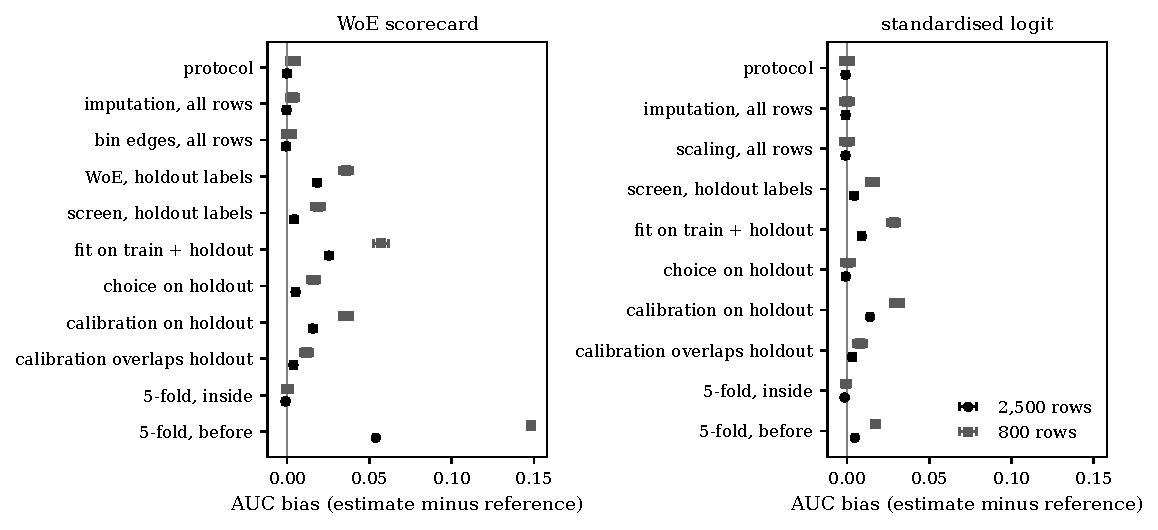
\includegraphics[width=\textwidth]{figures/fig-bias-by-leak.pdf}
\caption{Bias of the holdout AUC, the estimate minus the value of the same fitted model on the reference sample, with its 95\% half-width over repetitions, for the protocol and for every leaked variant, for the WoE scorecard (left) and the standardised logit (right) on planted data of 2,500 rows (circles) and of 800 rows (squares).}
\label{fig:bias-by-leak}
\end{figure}

The choice of a configuration on the holdout has a small cost. The scorecard chooses among eight configurations and its bias is \nv{syn.w.sel.bias}$\,\pm\,$\nv{syn.w.sel.ci} on the planted data and \nv{small.w.sel.bias} on the small sample; the logit chooses between two and its bias is \nv{syn.l.sel.bias} and \nv{small.l.sel.bias}. This is the pattern of Proposition~\ref{prop:selection}: with configurations that are strongly correlated the optimism is a small fraction of the bound $\sigma\sqrt{2\ln K}$, and it grows with $K$ and with the smaller holdout. The two five-fold procedures separate cleanly. Preprocessing inside the folds gives a bias of \nv{syn.w.cvin.bias}$\,\pm\,$\nv{syn.w.cvin.ci}; preprocessing on all development rows before the folds gives \nv{syn.w.cvpre.bias}$\,\pm\,$\nv{syn.w.cvpre.ci} on the planted data and \nv{small.w.cvpre.bias}$\,\pm\,$\nv{small.w.cvpre.ci} on the small sample, an optimism larger than that of every holdout leak on the planted data, because the binning, the weight of evidence and the screen of every fold were fitted with the validation rows of that fold. The logit, whose screen is a correlation that keeps ten of 40 inputs and which has no weight of evidence, gains less: \nv{syn.l.cvpre.bias} on the planted data and \nv{tw.l.cvpre.bias}$\,\pm\,$\nv{tw.l.cvpre.ci} on the card holders, where the interval contains zero.

\begin{figure}[htbp]
\centering
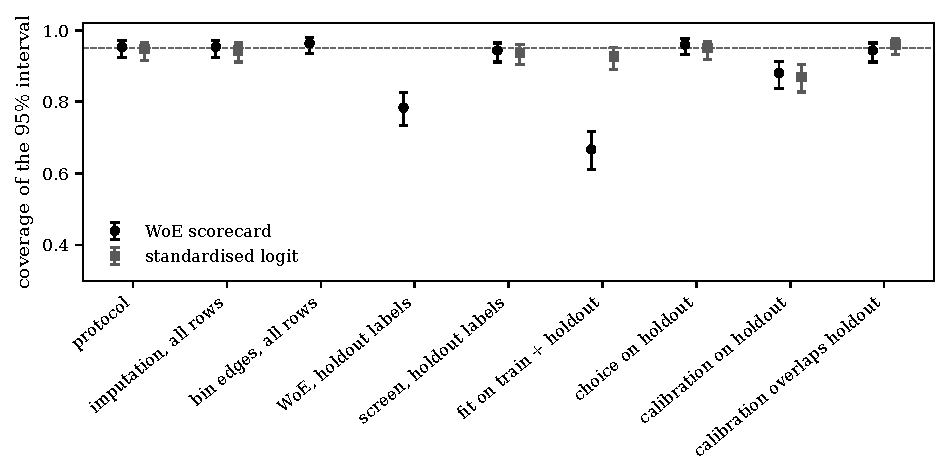
\includegraphics[width=\textwidth]{figures/fig-coverage.pdf}
\caption{Coverage of the engine's 95\% interval of the holdout AUC, the share of 300 repetitions in which the interval contains the reference value of the fitted model, for the WoE scorecard (circles) and the standardised logit (squares) on planted data of 2,500 rows, with Wilson intervals; the dotted line is the nominal 0.95.}
\label{fig:coverage}
\end{figure}

Figure~\ref{fig:coverage} shows what the leaks do to the interval that a validator reports. The leaks that read labels do not only move the point estimate: they leave the interval where it was, so that it fails to cover the reference value. For the scorecard the coverage falls to \nv{syn.w.woe.cov}\% for the weight of evidence with holdout labels, \nv{syn.w.fit.cov}\% for the fit on everything and \nv{syn.w.caltest.cov}\% for the calibration on the holdout, and for the product's own scorecard fitted on everything to \nv{prod.p.fit.cov}\% (Wilson interval \nv{prod.p.fit.covlo} to \nv{prod.p.fit.covhi}\%). A validator that reads the interval as a statement about the future is therefore misled by more than the point estimate suggests. Figure~\ref{fig:bias-distribution} gives the distribution of the bias in a repetition: the protocol is centred on zero with the spread of the sampling error of the holdout, and the leaked variants are the same distribution shifted to the right.

\begin{figure}[htbp]
\centering
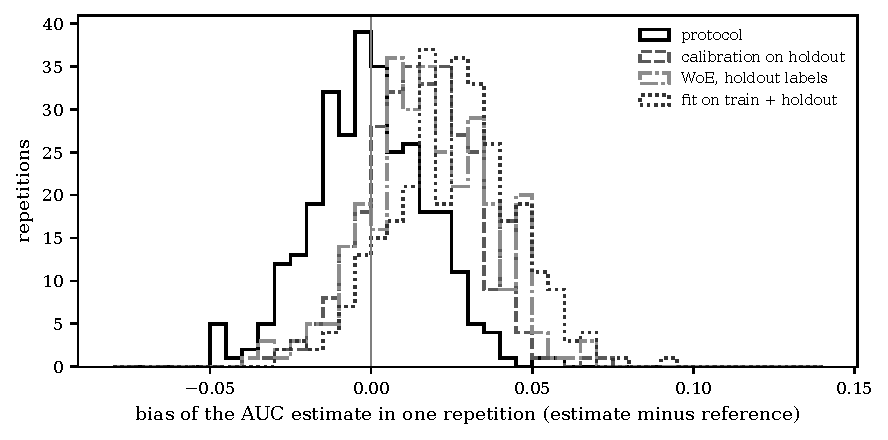
\includegraphics[width=0.85\textwidth]{figures/fig-bias-distribution.pdf}
\caption{Distribution over 300 repetitions of the bias of the holdout AUC in one repetition for the WoE scorecard on planted data of 2,500 rows: the protocol and three leaked variants, drawn as step histograms of the estimate minus the reference value of the fitted model.}
\label{fig:bias-distribution}
\end{figure}

\begin{table*}[htbp]
\centering
\small
\caption{Bias of the holdout AUC (with its 95\% half-width) and coverage of the 95\% interval in percent for the WoE scorecard on planted data of 800 rows (300 repetitions), on the 2,500-row subsamples of the 30,000 card holders of C01 (150 repetitions, 10,000 rows set aside per repetition as the reference), and for the product's own optbinning scorecard on planted data (90 repetitions; only the variants that call the product's fit appear).}
\label{tab:other-data}
\fitwidth{%
\begin{tabular}{lrrrrrr}
\toprule
Validation procedure & Small sample bias & Cov. & Card holders bias & Cov. & Product scorecard bias & Cov. \\
\midrule
proposed protocol & $+0.003\pm0.004$ & 95 & $+0.002\pm0.004$ & 93 & $+0.001\pm0.004$ & 93 \\
imputation on all rows & $+0.003\pm0.004$ & 95 & $+0.002\pm0.004$ & 93 & -- & -- \\
bin edges on all rows & $+0.001\pm0.004$ & 93 & $+0.002\pm0.004$ & 94 & -- & -- \\
WoE with holdout labels & $+0.036\pm0.004$ & 72 & $+0.015\pm0.004$ & 88 & -- & -- \\
screen with holdout labels & $+0.019\pm0.004$ & 89 & $+0.003\pm0.004$ & 93 & -- & -- \\
everything fitted on training and holdout & $+0.057\pm0.004$ & 54 & $+0.019\pm0.004$ & 85 & $+0.039\pm0.004$ & 36 \\
configuration chosen on the holdout & $+0.016\pm0.004$ & 91 & $+0.004\pm0.004$ & 94 & -- & -- \\
calibration map fitted on the holdout & $+0.036\pm0.004$ & 80 & $+0.020\pm0.004$ & 81 & $+0.016\pm0.004$ & 81 \\
calibration slice overlapping the holdout & $+0.012\pm0.004$ & 93 & $+0.007\pm0.004$ & 91 & -- & -- \\
five-fold, preprocessing inside the folds & $+0.000\pm0.003$ & -- & $+0.001\pm0.003$ & -- & -- & -- \\
five-fold, preprocessing before the folds & $+0.148\pm0.002$ & -- & $+0.016\pm0.003$ & -- & -- & -- \\
\bottomrule
\end{tabular}%
}
\end{table*}


Table~\ref{tab:other-data} shows that the pattern holds on the other data. On the small sample the effects are about twice as large, as the sampling noise that the leaked step fits is larger: the fit on everything adds \nv{small.w.fit.bias}$\,\pm\,$\nv{small.w.fit.ci} with a coverage of \nv{small.w.fit.cov}\%. On the card holders the effects are smaller (\nv{tw.w.fit.bias} for the fit on everything, \nv{tw.w.woe.bias} for the weight of evidence, \nv{tw.w.caltest.bias} for the calibration on the holdout), except that of the calibration, which is as large as on the planted data; the card holders have 20 inputs against 40, and the cross-validation results below show that the optimism of a leak that fits noise grows with the number of inputs. The screen with holdout labels adds \nv{tw.w.scr.bias}$\,\pm\,$\nv{tw.w.scr.ci} on the card holders, which is not distinguishable from zero. The second prediction required the three label-reading steps to inflate the AUC on every data set; it holds on the planted data (three of three) and on the small sample (three of three) and fails on the card holders (two of three), and it is reported as not held. The product's scorecard fitted on everything adds \nv{prod.p.fit.bias}$\,\pm\,$\nv{prod.p.fit.ci} and its calibration on the holdout \nv{prod.p.caltest.bias}$\,\pm\,$\nv{prod.p.caltest.ci}, so that the compact pipeline and the product's fit give the same sign and the same order of magnitude; the product's scorecard, whose binning is the optimal binning of its package, gains more from the fit on everything (\nv{prod.p.fit.bias} against \nv{syn.w.fit.bias}) and the same from the calibration on the holdout.

\subsection{What the gates detect}

Table~\ref{tab:gates} and Figure~\ref{fig:gate-matrix} give the share of \nv{e2.reps} draws in which each gate fails, for the leaks planted in the fitting path. On the protocol no gate fails in any draw, for either model, and the non-vacuity control is satisfied in every draw; with zero failures in \nv{e2.reps} draws, the Wilson upper bound of the false-alarm rate is \nv{e2.fa.upper}\%. The three gates are complementary. The first gate (transforms on the training slice only) fails in every draw for every leak that reads holdout rows in a transform (imputation, scaling, bin edges, weight of evidence, screen and the fit on everything), and it is blind to the calibration leaks (0\% for both). The second gate (calibration slice disjoint and invariant to the holdout labels) fails in every draw for the leaks that read labels and for the calibration leaks and, through the calibration map that depends on the chosen configuration, in \nv{e2.w.sel.G2}\% and \nv{e2.l.sel.G2}\% of the draws for the choice on the holdout (scorecard and logit); it is blind to the input-only leaks, imputation, scaling and bin edges (0\%). The third gate fails for every leak that the first two catch, except that against the choice on the holdout it has the power of Proposition~\ref{prop:discrete}.

\begin{table}[htbp]
\centering
\small
\caption{Share of 100 data draws of 1,500 rows in which each gate fails, so that the leak is detected: G1 moves the inputs outside the training slice, G2 requires disjoint slices and a calibration map unchanged when the holdout labels are flipped, G3 perturbs the holdout inputs and labels (one perturbation draw) and requires every fitted parameter unchanged. The first row of each model is the proposed protocol, where a failure is a false alarm.}
\label{tab:gates}
\fitwidth{%
\begin{tabular}{llrrrr}
\toprule
Model & Leak planted in the fitting path & G1 & G2 & G3 & Any gate \\
\midrule
WoE scorecard & none (false alarm rate) & 0 & 0 & 0 & 0 \\
 & imputation on all rows & 100 & 0 & 100 & 100 \\
 & bin edges on all rows & 100 & 0 & 100 & 100 \\
 & WoE with holdout labels & 100 & 100 & 100 & 100 \\
 & screen with holdout labels & 100 & 100 & 100 & 100 \\
 & everything fitted on training and holdout & 100 & 100 & 100 & 100 \\
 & configuration chosen on the holdout & 92 & 100 & 91 & 100 \\
 & calibration map fitted on the holdout & 0 & 100 & 100 & 100 \\
 & calibration slice overlapping the holdout & 0 & 100 & 100 & 100 \\
standardised logit & none (false alarm rate) & 0 & 0 & 0 & 0 \\
 & imputation on all rows & 100 & 0 & 100 & 100 \\
 & scaling on all rows & 100 & 0 & 100 & 100 \\
 & screen with holdout labels & 100 & 100 & 100 & 100 \\
 & everything fitted on training and holdout & 100 & 100 & 100 & 100 \\
 & configuration chosen on the holdout & 50 & 99 & 48 & 100 \\
 & calibration map fitted on the holdout & 0 & 100 & 100 & 100 \\
 & calibration slice overlapping the holdout & 0 & 100 & 100 & 100 \\
\bottomrule
\end{tabular}%
}
\end{table}


\begin{figure}[htbp]
\centering
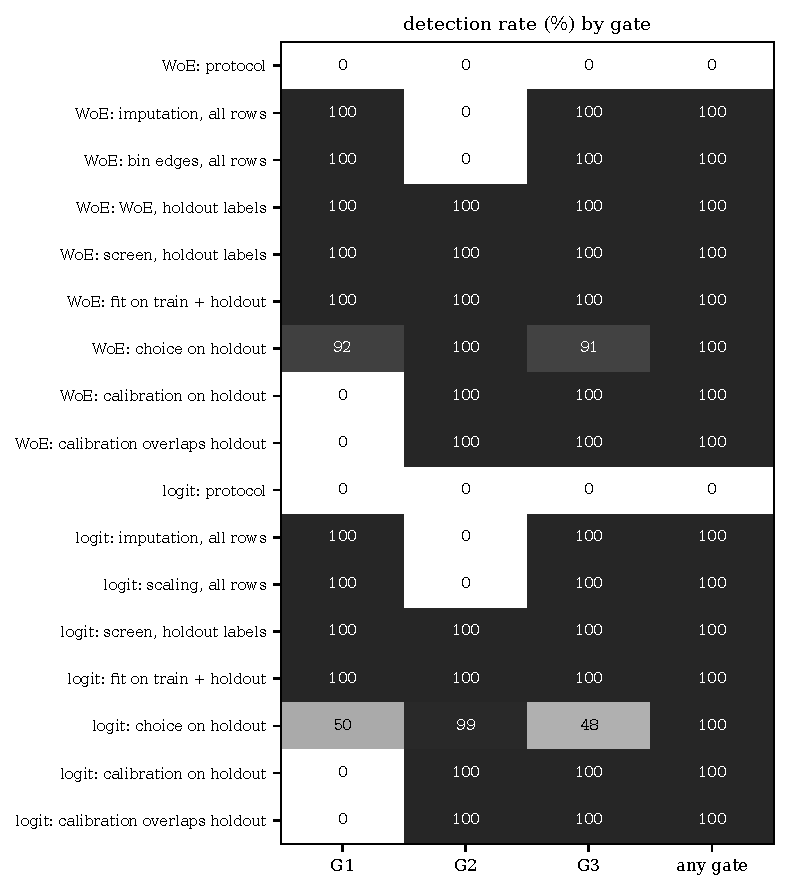
\includegraphics[width=0.62\textwidth]{figures/fig-gate-matrix.pdf}
\caption{Detection rate in percent of the three gates and of any of them for each leak planted in the fitting path of the WoE scorecard and of the standardised logit, over 100 draws of 1,500 rows; the first row of each model is the protocol, where a detection would be a false alarm.}
\label{fig:gate-matrix}
\end{figure}

At least one gate fails for every one of the \nv{h5.total} leaks in every draw (minimum over leaks \nv{h5.minany}\%) and none fails on the protocol, so that the fifth prediction holds. The leaks that read only holdout inputs are the instructive ones: the gates fail on them in every draw although their bias in Table~\ref{tab:main-results} is nil. A failure of a gate says that a rule was broken, not that the estimate is wrong; the bias that the rule protects against depends on the step, and the gates cannot tell a harmless breach from a harmful one. The choice of a configuration on the holdout is the case in which the third gate is partial: it fails in \nv{e2.w.sel.G3}\% of the draws for the scorecard, which chooses among eight configurations, and in \nv{e2.l.sel.G3}\% for the logit, which chooses between two. Figure~\ref{fig:detection-draws} (left) shows how repeating the perturbation raises the detection: with one, two, three and five draws the scorecard's choice is detected in \nv{e2.draws.w.1}, \nv{e2.draws.w.2}, \nv{e2.draws.w.3} and \nv{e2.draws.w.5}\% of \nv{e2.draws.reps} draws, against \nv{e2.draws.pred.w.1}, \nv{e2.draws.pred.w.2}, \nv{e2.draws.pred.w.3} and \nv{e2.draws.pred.w.5}\% for $1-K^{-d}$, and the logit's in \nv{e2.draws.l.1}, \nv{e2.draws.l.2}, \nv{e2.draws.l.3} and \nv{e2.draws.l.5}\% against \nv{e2.draws.pred.l.1}, \nv{e2.draws.pred.l.2}, \nv{e2.draws.pred.l.3} and \nv{e2.draws.pred.l.5}\%; the simulation has a standard error of up to \nv{e2.draws.se} points, and every observed rate is within \nv{e2.draws.zmax} standard errors of the prediction, each taken at its own predicted rate.

\begin{figure}[htbp]
\centering
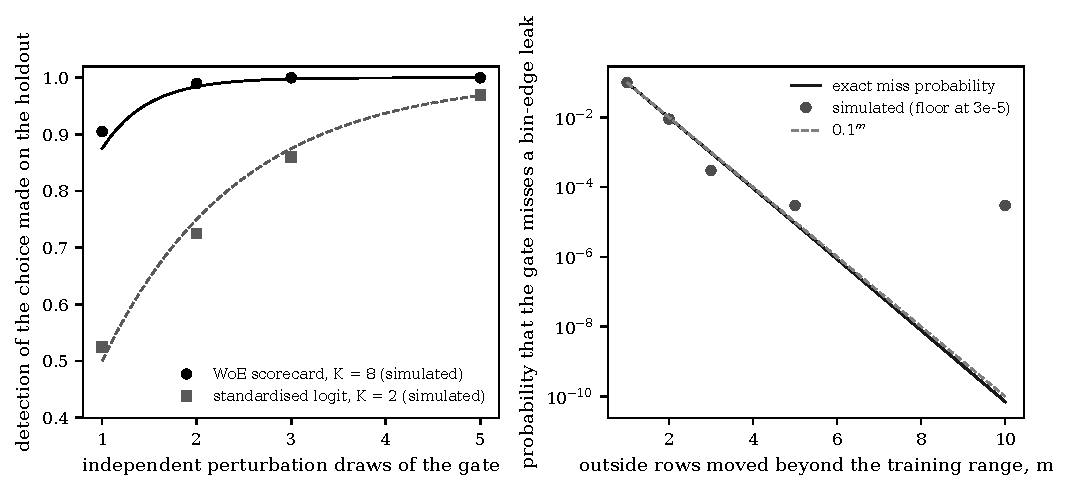
\includegraphics[width=\textwidth]{figures/fig-detection-draws.pdf}
\caption{Left: detection by the third gate of a choice made on the holdout, against the number of independent perturbation draws, for the scorecard (eight configurations) and the logit (two) in 200 draws of the data, with the curves $1-K^{-d}$ of Proposition~\ref{prop:discrete}. Right: probability that the gate misses a leak through a bin edge against the number of outside rows moved, simulated, exact (Proposition~\ref{prop:detection}) and $0.1^m$.}
\label{fig:detection-draws}
\end{figure}

\begin{table}[htbp]
\centering
\small
\caption{Probability that sending m outside rows beyond the training range changes at least one decile edge of a pooled sample of 1,500 rows (1,050 training and 450 outside), simulated with the pipeline's own edge function over 10,000 trials per row, against the exact hypergeometric expression and its approximation of Proposition 2.}
\label{tab:theory-detection}
\fitwidth{%
\begin{tabular}{lrrr}
\toprule
Perturbation of the outside rows & Simulated detection (\%) & Exact (\%) & $1-0.1^m$ (\%) \\
\midrule
edge shift, m = 1 & \relax 90.0 $\pm$ 0.6 & 90.07 & 90.00 \\
edge shift, m = 2 & \relax 99.1 $\pm$ 0.2 & 99.02 & 99.00 \\
edge shift, m = 3 & \relax 100.0 $\pm$ 0.0 & 99.90 & 99.90 \\
edge shift, m = 5 & \relax 100.0 $\pm$ 0.0 & 100.00 & 100.00 \\
edge shift, m = 10 & \relax 100.0 $\pm$ 0.0 & 100.00 & 100.00 \\
\bottomrule
\end{tabular}%
}
\end{table}


Table~\ref{tab:theory-detection} and the right panel of Figure~\ref{fig:detection-draws} check Proposition~\ref{prop:detection}: one outside row moved beyond the training range is detected in \nv{th.det.1.sim}\% of \nv{th.det.trials} trials against \nv{th.det.1.exact}\% from the exact expression, two in \nv{th.det.2.sim}\% against \nv{th.det.2.exact}\%, at three the simulation sees \nv{th.det.3.miss} misses in \nv{th.det.trials} trials against \nv{th.det.3.missexp} expected, which is the largest standardised difference, \nv{th.det.zmax}, over the five values of $m$, and from five upward it sees \nv{th.det.5.miss}. The approximation $1-0.1^m$ is a lower bound of the exact value, as the proof states. The gate moves the whole holdout, so its probability of missing a leak through a bin edge is not the limiting factor.

The product's own ladder confirms the pattern (Section~\ref{sec:experimental-design}). On the planted set of \nv{e2.ladder.n} rows, the protocol leaves \nv{e2.ladder.protocol.changed} of \nv{e2.ladder.protocol.rungs} rungs changed under the perturbation of the holdout; fitting the rungs on the training slice and the holdout changes \nv{e2.ladder.fit_on_train_and_holdout.changed} of \nv{e2.ladder.fit_on_train_and_holdout.rungs}; fitting the calibration maps on the holdout changes \nv{e2.ladder.calibration_on_holdout.changed} of \nv{e2.ladder.calibration_on_holdout.rungs}, the two rungs that carry a calibration map. The checks of the product's tests are therefore the gates of the experiments, and they have the same power in the seven-rung ladder.

\subsection{A leak that exists only in development}

\begin{figure}[htbp]
\centering
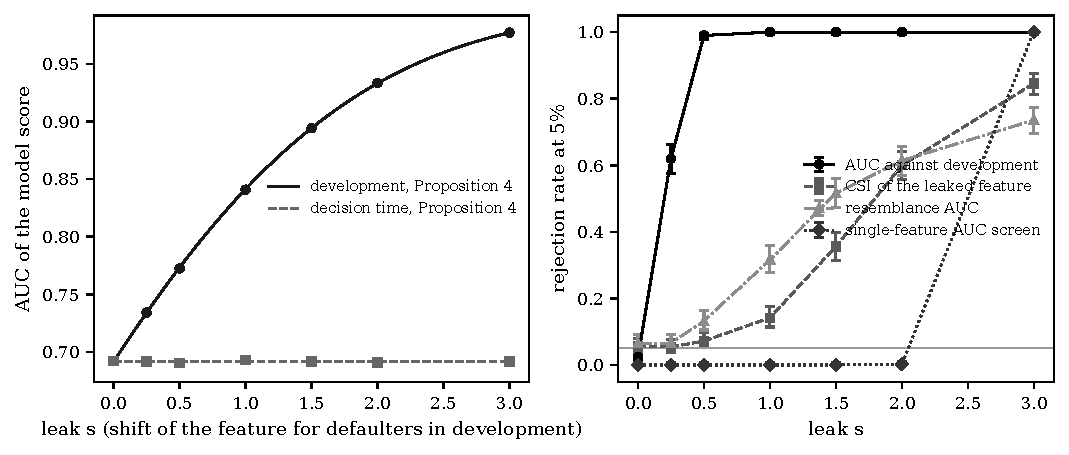
\includegraphics[width=\textwidth]{figures/fig-planted-leak.pdf}
\caption{The leak planted by the engine generator, with 150 defaulters and 4,850 survivors per sample: left, the simulated mean AUC in development and at decision time against the leak $s$ with the closed forms of Proposition~\ref{prop:leakauc}; right, the percentage of 500 repetitions in which each detector rejects at 5\%, with Wilson intervals.}
\label{fig:planted-leak}
\end{figure}

\begin{table*}[htbp]
\centering
\small
\caption{The leak planted by the engine generator (150 defaulters and 4,850 survivors per sample, 500 repetitions per level): simulated mean AUC in development and at decision time beside the closed forms of Proposition 4, and the percentage of repetitions in which each detector rejects at 5\%: the AUC-against-development test, the characteristic stability index of the leaked feature, the resemblance AUC and the single-feature AUC screen at its default threshold of 0.95.}
\label{tab:planted-leak}
\fitwidth{%
\begin{tabular}{rrrrrrrrr}
\toprule
Leak $s$ & Dev. AUC sim. & Dev. AUC Prop. & Current AUC sim. & Current AUC Prop. & AUC test power & CSI power & Resemblance power & Single-feature flag \\
\midrule
0 & 0.692 & 0.691 & 0.692 & 0.691 & 2.4 & 5.6 & 6.6 & 0.0 \\
0.25 & 0.734 & 0.734 & 0.692 & 0.691 & 62.0 & 5.4 & 6.6 & 0.0 \\
0.5 & 0.772 & 0.773 & 0.691 & 0.691 & 99.0 & 7.2 & 13.2 & 0.0 \\
1 & 0.841 & 0.841 & 0.693 & 0.691 & 100.0 & 14.2 & 31.6 & 0.0 \\
1.5 & 0.894 & 0.894 & 0.692 & 0.691 & 100.0 & 35.6 & 51.6 & 0.0 \\
2 & 0.933 & 0.933 & 0.691 & 0.691 & 100.0 & 60.0 & 61.4 & 0.2 \\
3 & 0.977 & 0.977 & 0.692 & 0.691 & 100.0 & 84.6 & 73.6 & 100.0 \\
\bottomrule
\end{tabular}%
}
\end{table*}


Table~\ref{tab:planted-leak} and Figure~\ref{fig:planted-leak} show what the engine's detectors see of a leak that is present in development and absent at decision time. The closed forms of Proposition~\ref{prop:leakauc} reproduce the simulated mean AUC at every level (the largest standardised difference over the seven levels is \nv{e3.zmax}, within three), and the development AUC is inflated by \nv{e3.s1.0.infl} at $s=1$ while the decision-time AUC does not move. The AUC-against-development test, which compares the current AUC with its development value, rejects in \nv{e3.s0.25.auc_test}\% of the repetitions at $s=0.25$, \nv{e3.s0.5.auc_test}\% at $s=0.5$ and \nv{e3.s1.0.auc_test}\% from $s=1$ upward, and at $s=0$ in \nv{e3.s0.0.auc_test}\%. The stability index of the leaked feature rejects in \nv{e3.s0.5.csi_test}\% at $s=0.5$, \nv{e3.s1.0.csi_test}\% at $s=1$ and \nv{e3.s2.0.csi_test}\% at $s=2$, against \nv{e3.s0.0.csi_test}\% under no leak. The committed document of the case, with \nv{c22.reps} repetitions per level, gives \nv{c22.csi.0.5}\%, \nv{c22.csi.1}\% and \nv{c22.csi.2}\% for the index at $s=0.5$, 1 and 2 and \nv{c22.auc.0.25}\%, \nv{c22.auc.0.5}\% and \nv{c22.auc.1}\% for the test against development at $s=0.25$, 0.5 and 1, which agrees with these rates; its null rate for the test against development is \nv{c22.auc.0}\% against \nv{e3.s0.0.auc_test}\% here (Wilson interval \nv{e3.s0.0.auc_lo} to \nv{e3.s0.0.auc_hi}\%), a difference of \nv{c22.null.diff} points (pooled two-proportion $z=\nv{c22.null.z}$, $p=\nv{c22.null.p}$) that the repetitions do not allow for and that this paper does not explain. Both rates are below the nominal 5\%, so the test is conservative at $s=0$ in these set-ups; at the leaked levels the two sets of rates agree. The resemblance AUC rejects in \nv{e3.s1.0.resemblance_flag}\% at $s=1$. The single-feature screen flags the leaked feature in \nv{e3.s1.0.single_feature_flag}\% at $s=1$ and in \nv{e3.s2.0.single_feature_flag}\% at $s=2$, because the feature alone has an AUC of \nv{e3.s1.0.feat} and \nv{e3.s2.0.feat}, below the threshold of 0.95; at $s=3$ the AUC of the feature is \nv{e3.s3.0.feat} and the screen flags it in \nv{e3.s3.0.single_feature_flag}\%. The sixth prediction holds: the test against development has a power of \nv{e3.s0.5.auc_test}\% at $s=0.5$ and the two feature-based detectors have \nv{e3.s1.0.csi_test}\% and \nv{e3.s1.0.single_feature_flag}\% at $s=1$. The explanation is Proposition~\ref{prop:psi}: the index of the leaked feature, \nv{th.psi.1.0.binned_chi2_form} at $s=1$ by the theory and \nv{th.psi.1.0.engine_psi} by the engine's exact value, is below the level of \nv{th.psi.null} that two samples of 5,000 rows produce by chance. The leak is a drop of discrimination out of time, not a drift of the feature.

\subsection{A random split against the out-of-time cohort}

\begin{figure}[htbp]
\centering
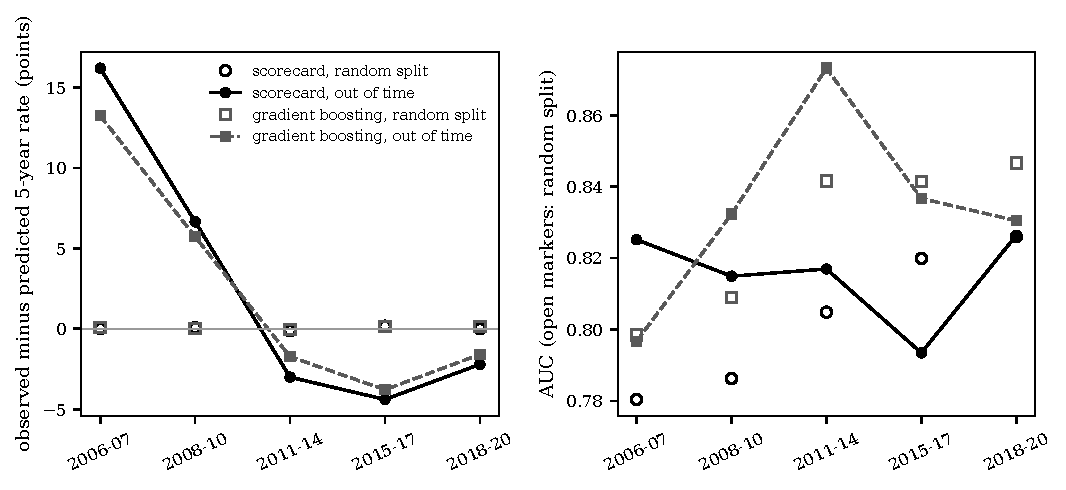
\includegraphics[width=\textwidth]{figures/fig-out-of-time.pdf}
\caption{For the five cohorts of the SBA 7(a) loans, left, the observed minus the predicted 5-year charge-off rate in percentage points of the scorecard and of the gradient-boosting rung on a random sample of the training window and on the out-of-time cohort; right, the AUC of the same rungs on the two samples (open markers: random split).}
\label{fig:out-of-time}
\end{figure}

\begin{table*}[htbp]
\centering
\small
\caption{Two estimates of the same fitted models on the SBA 7(a) loans of C03: a random sample of the training window's own loans that neither the fit nor the calibration used (rand.), and the declared out-of-time cohort at the 5-year mark of each vintage (OOT). The gap is the observed minus the predicted 5-year charge-off rate in percentage points; the columns are the WoE scorecard (Score.) and the monotone gradient-boosting rung (GBM), and the training window of each cohort is in the table of splits.}
\label{tab:out-of-time}
\fitwidth{%
\begin{tabular}{lrrrrrrrrr}
\toprule
Cohort & Window loans & \shortstack{Score.\\AUC rand.} & \shortstack{Score.\\AUC OOT} & \shortstack{Score.\\gap rand.} & \shortstack{Score.\\gap OOT} & \shortstack{GBM\\AUC rand.} & \shortstack{GBM\\AUC OOT} & \shortstack{GBM\\gap rand.} & \shortstack{GBM\\gap OOT} \\
\midrule
FY2006-07 & 330,682 & 0.780 & 0.825 & 0.0 & +16.2 & 0.799 & 0.797 & +0.1 & +13.2 \\
FY2008-10 & 413,083 & 0.786 & 0.815 & +0.1 & +6.6 & 0.809 & 0.832 & 0.0 & +5.7 \\
FY2011-14 & 627,594 & 0.805 & 0.817 & $-$0.1 & $-$3.0 & 0.842 & 0.873 & $-$0.1 & $-$1.7 \\
FY2015-17 & 900,254 & 0.820 & 0.793 & +0.2 & $-$4.4 & 0.841 & 0.837 & +0.1 & $-$3.8 \\
FY2018-20 & 1,024,597 & 0.826 & 0.826 & 0.0 & $-$2.2 & 0.847 & 0.830 & +0.1 & $-$1.6 \\
\bottomrule
\end{tabular}%
}
\end{table*}


Table~\ref{tab:out-of-time} and Figure~\ref{fig:out-of-time} compare, for the same fitted models, a random sample of the training window that the fit and the calibration did not read with the declared out-of-time cohort. On the random sample the level of the scorecard is right in every cohort: the gap between observed and predicted 5-year rates is between \nv{e4.2011-14.sc.random_gap} and \nv{e4.2015-17.sc.random_gap} points, within \nv{e4.maxz} binomial standard errors of the 60,000-loan sample at the window rate of each cohort (\nv{e4.sed.lo} to \nv{e4.sed.hi} points; \nv{e4.holdse} points is the largest value that a binomial standard error of this sample can take), for the scorecard and for the gradient-boosting rung. On the out-of-time cohort the gap is \nv{e4.2006-07.sc.oot_gap} points for the cohort of fiscal years 2006 and 2007, whose observed 5-year rate is \nv{e4.2006-07.rate_oot}\% against \nv{e4.2006-07.rate_random}\% in the window, \nv{e4.2008-10.sc.oot_gap} for 2008 to 2010, \nv{e4.2011-14.sc.oot_gap} for 2011 to 2014, \nv{e4.2015-17.sc.oot_gap} for 2015 to 2017 and \nv{e4.2018-20.sc.oot_gap} for 2018 to 2020; the gradient-boosting rung has gaps of the same sign and a smaller size, namely \nv{e4.2006-07.gbm.oot_gap}, \nv{e4.2008-10.gbm.oot_gap}, \nv{e4.2011-14.gbm.oot_gap}, \nv{e4.2015-17.gbm.oot_gap} and \nv{e4.2018-20.gbm.oot_gap}, which is below 2 points for the cohorts \nv{h8.failed}. A random split cannot see the shift of level, because the window it samples has the level of the window. The eighth prediction, applied to both rungs, does not hold: the random gap is below one point in \nv{h8.rand} of \nv{h8.cells} cohort and rung cells, and the out-of-time gap is at least two points in \nv{h8.oot} of \nv{h8.cells}, the exceptions being the two gradient-boosting cells named above. The scorecard clears the rule in every cohort, with a smallest out-of-time gap of \nv{c03.mingap} points, a value that the committed documents of the case already held. The AUC behaves differently and is not systematically optimistic: the out-of-time AUC of the scorecard is above the random-split AUC for the first three cohorts (\nv{e4.2006-07.sc.oot_auc} against \nv{e4.2006-07.sc.random_auc} for the first) and below it for 2015 to 2017 (\nv{e4.2015-17.sc.oot_auc} against \nv{e4.2015-17.sc.random_auc}). What the declared cohort measures, and the random split does not, is the level. The run reproduces the committed out-of-time AUC of the scorecard of every cohort to within \nv{e4.maxrepdiff}.

\subsection{Cross-validation with preprocessing outside the folds}

\begin{figure}[htbp]
\centering
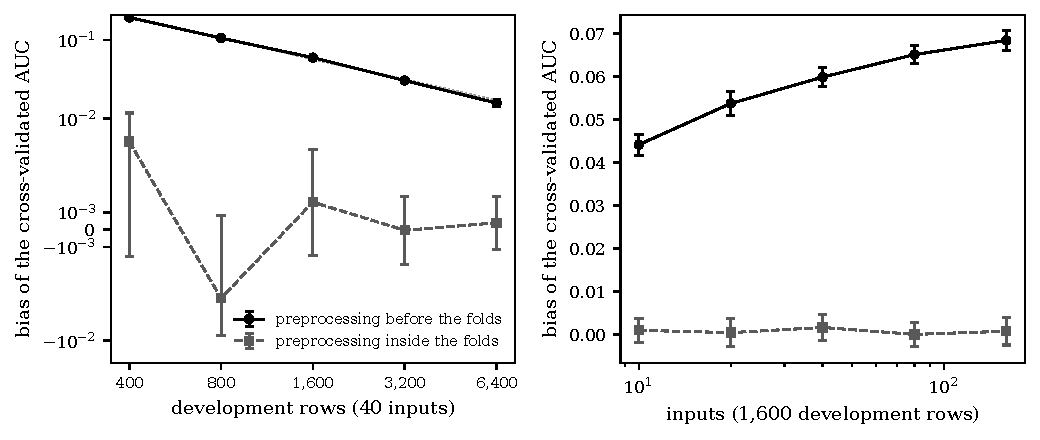
\includegraphics[width=\textwidth]{figures/fig-cv-scaling.pdf}
\caption{Bias of the five-fold AUC against the mean reference AUC of the fold models for the WoE scorecard on planted data, with preprocessing fitted inside each training fold (squares) or on all development rows before the folds (circles); left, against the number of development rows at 40 inputs on a symmetric logarithmic scale, with the fitted power law; right, against the number of inputs at 1,600 rows.}
\label{fig:cv-scaling}
\end{figure}

\begin{table}[htbp]
\centering
\small
\caption{Bias of five-fold cross-validated AUC against the mean reference AUC of the fold models for the WoE scorecard on planted data (five informative inputs, the rest noise), 100 repetitions per row, with the preprocessing fitted inside each training fold or on all development rows before the folds; the 95\% half-widths are over repetitions.}
\label{tab:cv-scaling}
\fitwidth{%
\begin{tabular}{rrrr}
\toprule
Development rows & Inputs & Preprocessing inside the folds & Preprocessing before the folds \\
\midrule
400 & 40 & $+0.005\pm0.007$ & $+0.194\pm0.005$ \\
800 & 40 & $-0.004\pm0.005$ & $+0.106\pm0.003$ \\
1,600 & 40 & $+0.002\pm0.003$ & $+0.060\pm0.002$ \\
3,200 & 40 & $0.000\pm0.002$ & $+0.031\pm0.002$ \\
6,400 & 40 & $+0.000\pm0.002$ & $+0.016\pm0.001$ \\
1,600 & 10 & $+0.001\pm0.003$ & $+0.044\pm0.002$ \\
1,600 & 20 & $+0.000\pm0.003$ & $+0.054\pm0.003$ \\
1,600 & 80 & $0.000\pm0.003$ & $+0.065\pm0.002$ \\
1,600 & 160 & $+0.001\pm0.003$ & $+0.068\pm0.002$ \\
\bottomrule
\end{tabular}%
}
\end{table}


Table~\ref{tab:cv-scaling} and Figure~\ref{fig:cv-scaling} give the bias of the five-fold AUC. With the preprocessing fitted inside each fold the bias is within the noise at all nine combinations (from \nv{e5.n800.p40.in} to \nv{e5.n400.p40.in}). With the preprocessing before the folds the bias is \nv{e5.n400.p40.out} at 400 development rows and falls to \nv{e5.n6400.p40.out} at 6,400, with a power-law slope of $-\nv{e5.exp}\pm\nv{e5.expse}$, from which the range of the exponent in the conjecture was read, so that the fit does not test it; at 1,600 rows it rises from \nv{e5.n1600.p10.out} at 10 inputs to \nv{e5.n1600.p160.out} at 160 and flattens. The ninth prediction, applied to both models on all three data sets, does not hold: the outside-fold bias is positive in \nv{h9.pos} of 6 pairs of data set and model and the inside-fold bias is null in \nv{h9.null} of 6. The exceptions are the logit on the card holders before the folds (\nv{tw.l.cvpre.bias}$\,\pm\,$\nv{tw.l.cvpre.ci}, not inflated) and the logit on the planted data inside the folds (\nv{syn.l.cvin.bias}$\,\pm\,$\nv{syn.l.cvin.ci}, a small negative bias); for the scorecard the contrast holds on all three data sets. The conjecture is consistent with the evidence and is not proved.

\subsection{Whether each prediction held}

Table~\ref{tab:hypotheses} gives the outcome of every prediction, applying each rule to every cell that the paper reports. Of the nine, \nv{h.held.word} held (H1, H3, H4, H5, H6 and H7) and \nv{h.notheld.word} did not (H2, H8 and H9). The second did not: on the card holders the screen with holdout labels does not raise the AUC beyond the noise (\nv{tw.w.scr.bias}$\,\pm\,$\nv{tw.w.scr.ci}), so that the claim that every label-reading step inflates the estimate is established for the weight of evidence and for the fit on everything and is not established for the screen on this data set. The eighth did not: the out-of-time gap of the gradient-boosting rung is below 2 points in two of the five cohorts, so that the contrast between a random split and the declared cohort holds at the size of two points for the scorecard and not for a second model. The ninth did not: the logit is not inflated by preprocessing before the folds on the card holders and is slightly negative inside the folds on the planted data, so that the contrast holds for the scorecard on every data set and not for the logit on every one. The third prediction held, and its holding is a limit of the claim that leaks inflate the estimate: the leaks through inputs only did not. The seventh held with a largest standardised difference of \nv{e3.zmax}, and the closed forms of the theory are reproduced by the generator. The sixth and the eighth were set with committed values of the cases in view (Section~\ref{sec:experimental-design}), so that the sixth is a reproduction of those values by new runs and the eighth a check that the scorecard clears a threshold placed at them. Two readings follow. The three failures concern the direction and size of an effect for one step, one rung or one model on one data set, and they do not touch the propositions, which make no claim about the screen on any data set, about the gradient-boosting rung or about the logit. The holding of the third prediction and of the scorecard rows of the ninth says that the rule on inputs and the rule on folds differ in kind: the first has no measurable cost in the estimate, and the second is the largest cost measured.

\section{Ablation}
\label{sec:ablation}

The protocol has components of two kinds: the rules on the row sets that the split enforces, and the gates that test the rules. Two ablations separate what each contributes. The first removes one rule at a time and reads the cost in the bias and the coverage of the resulting leak. The second keeps every subset of the gates and reads what the subset detects.

\subsection{Removing one rule of the split}

Table~\ref{tab:ablation-components} gives, for each rule that is removed, the worst of the leaks that the removal allows. The rule that the statistics are fitted on the training slice only is the most valuable: its removal in the whole fitting path adds \nv{syn.w.fit.bias}$\,\pm\,$\nv{syn.w.fit.ci} to the AUC and lowers the coverage of the interval to \nv{syn.w.fit.cov}\%. The value is not spread evenly over the steps. Of the five steps whose removal is covered by this rule, two cost nothing measurable on the planted data (imputation, \nv{syn.w.imp.bias}, and bin edges, \nv{syn.w.bin.bias}); the screen costs \nv{syn.w.scr.bias}; and the weight of evidence costs \nv{syn.w.woe.bias}, which is more than two thirds of the cost of reading the holdout in every step, so that the target-aware transform is where a scorecard is most exposed. The rule that the configuration is chosen inside the training slice is the cheapest: its removal costs \nv{syn.w.sel.bias}$\,\pm\,$\nv{syn.w.sel.ci} with eight configurations and nothing measurable with two, which is the behaviour of Proposition~\ref{prop:selection} for correlated configurations. The rule that the calibration slice is disjoint from the test slice costs \nv{syn.w.caltest.bias}$\,\pm\,$\nv{syn.w.caltest.ci} in AUC, lowers the coverage to \nv{syn.w.caltest.cov}\% and is the only rule whose removal makes the calibration error look better than it is. The rule that the cross-validation folds contain the preprocessing is the most expensive when a scorecard is validated by cross-validation rather than by a holdout, with \nv{syn.w.cvpre.bias}$\,\pm\,$\nv{syn.w.cvpre.ci}; on the small sample it reaches \nv{small.w.cvpre.bias}. No rule is redundant for the estimate: each removal produces a bias whose interval excludes zero on the planted data, except the two input-only steps, and those are the ones that cost nothing in bias while a gate still fails on them.

\begin{table}[htbp]
\centering
\small
\caption{Removing one component of the protocol at a time on the planted data of the main comparison (WoE scorecard): the leak that results from the removal with the largest AUC bias, its bias with the 95\% half-width, the coverage of the 95\% interval and the Brier bias. The reference row of the protocol is in the main comparison table.}
\label{tab:ablation-components}
\fitwidth{%
\begin{tabular}{llrrr}
\toprule
Component of the protocol removed & Worst resulting leak & AUC bias & Coverage \% & Brier bias \\
\midrule
Statistics fitted on the training slice only & everything fitted on training and holdout & $+0.025\pm0.002$ & 66.7 & $-$0.0088 \\
Configuration chosen inside the training slice & configuration chosen on the holdout & $+0.005\pm0.002$ & 96.0 & $-$0.0018 \\
Calibration slice disjoint from the test slice & calibration map fitted on the holdout & $+0.016\pm0.002$ & 88.0 & $-$0.0081 \\
Preprocessing inside the cross-validation folds & five-fold, preprocessing before the folds & $+0.054\pm0.001$ & -- & -- \\
\bottomrule
\end{tabular}%
}
\end{table}


\subsection{Keeping a subset of the gates}

Table~\ref{tab:ablation-gates} gives the detection of every subset of the three gates over the \nv{h5.total} leaks planted in the fitting path. No subset has a false alarm on the protocol (\nv{abl.G1G2G3.fa}\% in every row), so the choice among subsets is a choice among powers. Each gate alone has a blind spot. The first gate alone detects \nv{abl.G1.full} of the \nv{h5.total} leaks in every draw and never detects \nv{abl.G1.never}: the calibration leaks, whose fitted parameters before the calibration map do not depend on the holdout. The second gate alone detects \nv{abl.G2.full} and never detects \nv{abl.G2.never}: the leaks through inputs only, imputation and bin edges for the scorecard and imputation and scaling for the logit, whose fitted values do not depend on labels. The third gate alone detects \nv{abl.G3.full} of the \nv{h5.total} in every draw and misses none altogether, with a mean detection of \nv{abl.G3.mean}\%; what it does not catch in every draw is the choice among configurations made on the holdout (Proposition~\ref{prop:discrete}). The pair of the second and the third gates detects all \nv{abl.G2G3.full} leaks in every draw, and the first gate adds nothing to this pair on the planted leaks. The first gate is nevertheless kept: it localises a failure to a transform instead of the calibration map.

\begin{table}[htbp]
\centering
\small
\caption{Ablation of the gates over the 15 leaks planted in the compact pipeline (100 draws each): the number of leaks that at least one gate of the subset detects in every draw, the number never detected by any gate of the subset, the mean over leaks of the share of draws in which at least one gate of the subset fails, and the largest false alarm rate on the protocol.}
\label{tab:ablation-gates}
\fitwidth{%
\begin{tabular}{lrrrr}
\toprule
Gates kept & Leaks always detected & Leaks never detected & Mean detection \% & False alarm \% \\
\midrule
G1 only & 9 of 15 & 4 & 69.5 & 0 \\
G2 only & 10 of 15 & 4 & 73.3 & 0 \\
G3 only & 13 of 15 & 0 & 95.9 & 0 \\
G1 and G2 & 14 of 15 & 0 & 99.9 & 0 \\
G1 and G3 & 14 of 15 & 0 & 98.0 & 0 \\
G2 and G3 & 15 of 15 & 0 & 100.0 & 0 \\
G1, G2 and G3 & 15 of 15 & 0 & 100.0 & 0 \\
\bottomrule
\end{tabular}%
}
\end{table}


The cost follows from equation~\eqref{eq:cost}: the pair of the second and the third gates needs the base fit, one fit for the flipped labels and $d$ fits for the perturbation draws, and the control one more, so that dropping the first gate saves one fit of the whole path out of $4+d$. The saving is small and the first gate stays in the protocol. The non-vacuity control passes in every draw for every variant of the experiments (\nv{e2.w.none.nv}\% for the scorecard under the protocol), so that none of the passes reported above is a pass of a pipeline that ignores its data; the control is not ablated, since a pipeline that fails it is defective and not leaky.

The ablation also shows what the protocol does not do. It does not choose, among the leaks, those that matter: a gate fails with the same certainty for imputation on all rows, which costs nothing in bias, as for the weight of evidence with holdout labels, which costs \nv{syn.w.woe.bias}. The ranking of the leaks by cost is the one of Table~\ref{tab:main-results}, not the one of Table~\ref{tab:gates}. A validator who finds that the first gate failed has found a breach of the rule and has to read the bias table to know what it costs in the step that failed.

\section{Discussion}
\label{sec:discussion}

\paragraph{The size of the cost depends on the step and on the sample.} The results say that the holdout of the protocol is an unbiased estimate of the fitted model's AUC, and that breaking the rules does not cost the same everywhere. A step that reads only inputs costs nothing measurable in the estimate (twelve of twelve cells); a step that reads labels costs between \nv{syn.w.scr.bias} (the screen) and \nv{syn.w.fit.bias} (every step) on 2,500 planted rows, and about twice as much on 800 rows; a calibration map fitted on the holdout costs about as much as the weight of evidence with holdout labels, and unlike the other leaks it makes the calibration error look better than it is. The ordering follows the flexibility of the step. A weight of evidence has ten free values per input, a screen picks ten of 40 inputs by their association with the label, a scaling has two parameters per input. The ordering is consistent with the optimism of an in-sample statistic, which grows with the number of quantities fitted from the rows that the estimate later reads, and the dependence on the sample size in the conjecture of Section~\ref{sec:theory} is the same mechanism seen through the cross-validation.

\paragraph{Why the interval misleads more than the point estimate.} The coverage of the engine's interval falls to \nv{syn.w.fit.cov}\% and, for the product's own scorecard, to \nv{prod.p.fit.cov}\% when every step reads the holdout. The interval is the DeLong interval, which describes the sampling variability of the AUC of a fixed model on a holdout. A leak does not change that variability; it shifts the centre by an amount of the order of the interval's half-width, so that the interval is a statement about the sampling error of a number that is already biased. A validator who reads the interval as the range in which the future AUC lies gets a range that excludes the future most of the time.

\paragraph{What the gates tell a validator and what they do not.} The gates fail whenever a rule is broken and they fail with the same certainty whatever the cost of the breach. The leak through imputation on all rows costs nothing in the estimate and fails two gates in every draw. For a validator the useful reading is that a failure localises the breach (a transform, the calibration map or the choice among configurations) and that the bias table says what that kind of breach has cost on data of the same shape. A protocol that reported only the cost would let a harmless leak pass, and a pipeline that is harmless on one sample can be harmful on another, as the doubling of the effects on the small sample shows. The gate that fails on a harmless breach is the price of a test that does not depend on the data.

\paragraph{Discrete choices need more than one draw.} The only leak that the third gate does not catch in every draw at its default setting is the choice of a configuration on the holdout, and Proposition~\ref{prop:discrete} says why: with two configurations a perturbed choice agrees with the base choice half of the time. The measurement agrees with the proposition (\nv{e2.draws.l.1}\% with one draw for the logit and \nv{e2.draws.l.5}\% with five), and the practical rule is that a pipeline that chooses among $K$ configurations needs $d$ draws with $K^{-d}$ below the miss probability that the validator accepts: five draws bring the detection of a choice among two configurations to \nv{e2.draws.pred.l.5}\% by the proposition, and two draws bring that of a choice among eight to \nv{e2.draws.pred.w.2}\%. The second gate catches the same leak in \nv{e2.w.sel.G2}\% and \nv{e2.l.sel.G2}\% of the draws through the calibration map, so that the protocol with all three gates detects it in every draw, but the dependence of that detection on the map is an accident of the pipeline and not a guarantee.

\paragraph{What the engine's tests see of a leak that exists only in development.} The planted leak shows a division of labour that a validation function should keep in mind. A test that compares the current AUC with the development AUC sees the leak at a shift of half a standard deviation (\nv{e3.s0.5.auc_test}\%); the stability index of the leaked feature sees it \nv{e3.s1.0.csi_test}\% of the time at a shift of one, and the single-feature screen not at all. A monitoring process that tracks input drift would therefore report a stable input and a falling AUC, so that a stable input does not certify the absence of a feature that carries the outcome in development and not at decision time. Proposition~\ref{prop:psi} says that this is not an accident of the generator: the index of a feature that is informative for a small share of the rows is second order in that share. The consequence for the practice that the protocol serves is that the leak that the gates cannot reach, a feature built from information dated after the observation date, has to be sought where it shows, in the discrimination out of time, and that a model whose development AUC is much higher than its AUC on the first cohort that follows is suspect before it is drifted.

\paragraph{A declared cohort measures the level, and a random split does not.} On the loan data a random sample of the training window gives the right level of the 5-year rate in every cohort, within \nv{e4.holdse} points, and the declared out-of-time cohort gives gaps of up to \nv{e4.2006-07.sc.aoot_gap} points. The AUC does not show the same pattern, and a random split is not systematically optimistic in discrimination on these data, which is consistent with a rank order that is more stable across vintages than the level of the default rate. For the provisions and the capital that use the PD as a level, the split that matters is the declared cohort, and a case that has none, as the card holders and the Polish bankruptcy files do, states that it makes no out-of-time claim instead of leaving the reader to assume it.

\paragraph{Negative and limiting results.} One prediction did not hold: the screen with holdout labels does not raise the AUC on the card holders, so the claim that every step that reads labels inflates the estimate is not established for that step on that data set. The leaks through inputs only do not inflate the estimate in any of the twelve cells, so the cost of a leak cannot be inferred from the fact of the breach. The choice among two configurations on the holdout costs nothing measurable. And a closed form that was expected to be accurate for the continuous index (Proposition~\ref{prop:psi}) is accurate only to a shift of one half; the binned form is the one to use. These limits narrow the claim of the paper to the one the results sustain: with the rules enforced and tested, the holdout number is unbiased and its interval covers; without them, the cost depends on the step and the sample, and the gates detect the breach whatever its cost.

\paragraph{Where the protocol sits in the practice of a validation function.} The protocol is a part of what a validator does before reading a holdout AUC. It is cheap ($4+d$ fits of the pipeline), it needs no change of the model and it yields a result that can be written to the artifact of a case, with the split and its limits. It is not a substitute for the review of the features for information from the future, for the out-of-time cohort where the data allow one, or for the discrimination test against the development value that the supervisory instructions ask for. The results of Section~\ref{sec:results} show that each of these sees something that the others do not.

\section{Limitations}
\label{sec:limitations}

The limits of the work are grouped as threats to internal, external and construct validity, followed by the scope that the protocol does not cover.

\paragraph{Internal validity.} The reference sample of each experiment is a finite sample, and the bias is measured against it. For the planted data its sampling error in the AUC is \nv{syn.orcse}, mean-zero across repetitions and negligible next to the half-widths reported; for the card holders it is \nv{tw.orcse} per repetition, which leaves the bias unchanged and makes the coverage of the interval on that data set slightly understated, since the interval is not widened for the error of the reference. The predictions of Table~\ref{tab:hypotheses} are fixed in the table script and their outcomes are computed from the committed outputs; they were not registered outside the repository, and the thresholds are round values chosen by the author, so that a reader who prefers other thresholds can apply them to the measured quantities of the table. The gates compare parameters by exact equality, which presupposes a deterministic fit; a pipeline with uncontrolled randomness, such as a multi-threaded fit with a non-deterministic reduction, would fail them without a leak, and the measured zero false-alarm rate holds for the compact pipeline and the product's ladder with their seeds. The third gate perturbs the holdout in a way that is fixed by equation~\eqref{eq:perturb}: a leak whose dependence on the holdout is unchanged by a redraw of the inputs from that law and of the labels from a fair coin passes the gate although it reads the holdout, and the perturbation family is part of the definition of the gate. The out-of-time experiment has one fit per cohort with the seed of the committed documents; its uncertainty is the binomial error of the 60,000-loan sample and the 5-year rate of the cohort, not the variability of the fit, which is not measured.

\paragraph{External validity.} The planted data are Gaussian with independent inputs and missingness completely at random; the card holders are a single snapshot with 20 numeric inputs; the loan files cover one lender programme. The fitting path is a WoE scorecard and a standardised logit, with the product's scorecard and ladder on planted data for the gates. The size of the bias of each leak is a property of these pipelines and these samples: the doubling from 2,500 to 800 rows and the difference between the planted data and the card holders show how much it moves. The measurement does not cover a gradient-boosting model, a neural network, a leak through a text or image feature, or the calibration by Platt scaling instead of isotonic regression. The gates are checked on the seven rungs of the product's ladder for the three conditions of its tests, not for every leak of the matrix.

\paragraph{Construct validity.} The estimand is the AUC of the fitted model on the population from which the development data are drawn. For the planted data that population is known; for the card holders it is the 30,000 rows of the snapshot, so that the reference is not the future of the card portfolio. The AUC-against-development test of the planted-leak experiment is the ECB form that takes the development AUC as known, with the exact development AUC of the generator; a validator who estimates the development AUC from a sample has a test with less power and, when the development sample is as large as the current one, a rejection rate under the null of about 11\% at the 5\% level, as the engine's documentation measures. The detectors of the planted leak are the engine's implementations of the single-feature screen and the resemblance test. The open toolkits whose tests share their purpose were not run: the paper compares with the practices that they exhibit or that their tests target, using the engine's equivalents, and a comparison with the toolkits' own code would need a data set on which their conventions and thresholds could be set equal to those of the engine. The nine leaks of the matrix are those that a pipeline of these steps allows; a leak through a step that is not in the compact pipeline, such as a feature selection by recursive elimination or a sampling correction before the split \citep{goorbergh2022}, is outside the measurement.

\paragraph{Scope of the protocol.} The protocol tests the dependence of the fitted parameters on rows outside the training information set. It does not test whether the training information set is free of information from the future: a feature that is built from data dated after the observation date is in the training rows and moves no parameter when the holdout moves, so that all gates pass. It does not test duplicates and near-duplicates across the slices, nor the dependence between rows of the same obligor, which makes assumption A1 false for panel data. It does not decide whether the cohort at which a dated case tests the model resembles the cohort in which it will be used, and it gives no guarantee for a pipeline whose fitting steps are not those of the experiments. A pass certifies that the perturbations of equations~\eqref{eq:g1} to~\eqref{eq:g3} found no dependence; it does not certify the absence of every leak.

\section{Reproducibility}
\label{sec:reproducibility}

All code, the committed outputs of the experiments and the sources of the tables and figures are in the repository \texttt{github.com/\allowbreak{}fsantibanezleal/\allowbreak{}CAOS\_\allowbreak{}Contraste}, in the folder \texttt{manuscripts/\allowbreak{}leakage-safe-validation-protocol}. The product release that holds these files and the committed outputs is release v1.00.000 of CAOS\_\allowbreak{}Contraste, tag v1.00.000. The engine is \texttt{riskvalidation} 1.1.0 with the market, ml and stress extras, and the pipeline is the product's \texttt{data-pipeline}. Every command below runs from the root of the repository with \texttt{python}. The card-holder and loan data are read from the data root named by the environment variable \texttt{CONTRASTE\_\allowbreak{}DATA}, and the cache of the card-holder sample from \texttt{CAOS\_\allowbreak{}TEMP\_\allowbreak{}ROOT} or from the argument \texttt{--cache}; nothing is written inside the repository except the committed outputs. % voice-ok: citation of the product release the results were produced with

The experiments are, in order:

\begin{itemize}
\item \texttt{experiments/\allowbreak{}e1\_\allowbreak{}estimator\_\allowbreak{}bias.py --dataset synthetic --reps 300}, and the same with \texttt{synthetic-small} (300 repetitions), \texttt{taiwan} (150) and \texttt{product} (90); it writes \texttt{experiments/\allowbreak{}results/\allowbreak{}e1\_\allowbreak{}<dataset>.json}.
\item \texttt{experiments/\allowbreak{}e2\_\allowbreak{}gates.py matrix --reps 100}, \texttt{draws --reps 200} and \texttt{ladder}; the outputs are \texttt{e2\_\allowbreak{}matrix.json}, \texttt{e2\_\allowbreak{}draws.json} and \texttt{e2\_\allowbreak{}ladder.json}.
\item \texttt{experiments/\allowbreak{}e3\_\allowbreak{}planted\_\allowbreak{}leak.py --reps 500}, which writes \texttt{e3\_\allowbreak{}planted\_\allowbreak{}leak.json}.
\item \texttt{experiments/\allowbreak{}e4\_\allowbreak{}out\_\allowbreak{}of\_\allowbreak{}time.py}, which fits the five cohorts of the loan case, checks the out-of-time AUC of the scorecard against the committed documents and writes \texttt{e4\_\allowbreak{}out\_\allowbreak{}of\_\allowbreak{}time.json}.
\item \texttt{experiments/\allowbreak{}e5\_\allowbreak{}cv\_\allowbreak{}scaling.py --reps 100} and \texttt{experiments/\allowbreak{}theory\_\allowbreak{}checks.py}, which write \texttt{e5\_\allowbreak{}cv\_\allowbreak{}scaling.json} and \texttt{theory\_\allowbreak{}checks.json}.
\end{itemize}

The table script \texttt{make\_\allowbreak{}artifacts.py} reads these outputs and the committed documents of the cases C01, C02, C03 and C22 under \texttt{data/\allowbreak{}derived}, and writes every table, the number macros of \texttt{tables/\allowbreak{}numbers.tex} and their sources in \texttt{tables/\allowbreak{}numbers.json}; every measured number in the text of this paper is read from that file, and the design constants (sizes of samples, thresholds, perturbation law) are stated in the text and in the scripts. The figure script \texttt{make\_\allowbreak{}figures.py} writes the vector figures. The references are rebuilt by \texttt{fetch\_\allowbreak{}references.py}, which fetches every record from its DOI or opens its address. The seeds are those of Table~\ref{tab:design}; every repetition derives its own seed, so the outputs do not depend on the number of workers.

Wall-clock times on a machine with 32 logical processors, with the experiments run in parallel over repetitions: the bias experiment on the planted data took \nv{run.e1syn} seconds for \nv{syn.n} rows and \nv{run.e1small} seconds for \nv{small.n} rows, \nv{run.e1tw} seconds on the card holders and \nv{run.e1prod} seconds for the product's scorecard; the gate matrix took \nv{run.e2matrix} seconds and the repeated-perturbation study \nv{run.e2draws} seconds; the planted leak took \nv{run.e3} seconds; and the longest of the five cohorts of the loan case took \nv{run.e4max} seconds, the cohorts running in parallel. The outputs are committed as compact JSON, so that the tables and figures are rebuilt without rerunning the experiments.

\section{Conclusions}
\label{sec:conclusions}

The paper measures a protocol that makes the holdout number of a credit-risk validation trustworthy: a split declared per case, a rule that fixes the training window of a dated case, and three invariance gates, with a control against vacuous passes, that fail when a fitted parameter depends on rows outside the training information set. Under the protocol, the holdout AUC of a WoE scorecard on planted data has a bias of \nv{syn.w.none.bias}$\,\pm\,$\nv{syn.w.none.ci} and its 95\% interval covers the reference value in \nv{syn.w.none.cov}\% of \nv{syn.reps} repetitions; the same holds for the standardised logit, on 800 rows, on the card holders and for the product's own scorecard. When a step reads the holdout the cost depends on the step: nothing measurable for imputation, scaling and bin edges, \nv{syn.w.woe.bias} for the weight of evidence with holdout labels and \nv{syn.w.fit.bias} when every step reads it, with coverage falling to \nv{syn.w.fit.cov}\%; a calibration map fitted on the holdout adds \nv{syn.w.caltest.bias} and makes the calibration look better than it is. Five-fold cross-validation with the preprocessing outside the folds is the most optimistic procedure measured (\nv{syn.w.cvpre.bias} on the planted data and \nv{small.w.cvpre.bias} on the small sample).

At least one of the three gates fails for each of the \nv{h5.total} leaks planted in the fitting path in every one of \nv{e2.reps} draws, and none fails on the protocol. The gates are complementary (the first misses the calibration leaks, the second the input-only leaks, the third a choice among configurations in a single draw), and they detect a breach of a rule whatever its cost. For a choice among configurations on the holdout, repeated perturbation gives a detection of $1-K^{-d}$, which the simulation reproduces within \nv{e2.draws.zmax} standard errors.

A leak that exists only in development is a drop of discrimination out of time and not a drift of the feature: the test of the current AUC against the development value rejects in \nv{e3.s0.5.auc_test}\% of the repetitions at a shift of half a standard deviation, while the stability index of the leaked feature rejects in \nv{e3.s1.0.csi_test}\% and the single-feature screen in \nv{e3.s1.0.single_feature_flag}\% at a shift of one, which the second-order form of the index explains. On five cohorts of the loan data a random split inside the training window reproduces the level of the 5-year rate within \nv{e4.maxz} binomial standard errors (at most \nv{e4.holdse} points) and the declared out-of-time cohort shows gaps of up to \nv{e4.2006-07.sc.aoot_gap} points.

Of the nine predictions, \nv{h.held.word} held and \nv{h.notheld.word} did not. The inflation by the screen with holdout labels on the card holders narrows the claim about label-reading steps to the weight of evidence and the fit on everything; the out-of-time gap of at least two points holds for the scorecard and not for the gradient-boosting rung in two cohorts; and the contrast of cross-validation inside and outside the folds holds for the scorecard on every data set and not for the logit on the card holders (before the folds) and on the planted data (inside the folds). The predictions were written together with the outputs that decide them, and H6 and H8 were set with committed values in view. The next steps are the measurement of the same gates on a gradient-boosting and a neural challenger, the extension of the leaks to the features built from dated information, where the gates are blind, and the measurement of the gates on a case with panel structure, where the exchangeability that the first proposition needs does not hold.


\bibliographystyle{plainnat}
\bibliography{references}

\end{document}
